\documentclass[11pt,letterpaper]{article}

\usepackage[utf8]{inputenc}
\usepackage[T1]{fontenc}
\usepackage{mathptmx}
\usepackage[margin=1in]{geometry}
\usepackage{amsmath,amssymb,amsthm}
\usepackage{booktabs}
\usepackage{microtype}
\usepackage{setspace}
\usepackage[round,authoryear]{natbib}
\usepackage{titlesec}
\usepackage{enumitem}
\usepackage{xcolor}
\usepackage{array}
\usepackage{tabularx}
\usepackage[colorlinks=true,linkcolor=red!70!black,citecolor=red!70!black,urlcolor=blue!70!black]{hyperref}
\usepackage{graphicx}
\usepackage{caption}
\captionsetup{font=small,labelfont=bf,skip=8pt}

\onehalfspacing
\setlength{\parskip}{0.3em}
\setlength{\parindent}{1.5em}

\titlespacing*{\section}{0pt}{1.4em}{0.6em}
\titlespacing*{\subsection}{0pt}{1em}{0.4em}

\newtheorem{proposition}{Proposition}
\theoremstyle{remark}
\newtheorem*{proof_sketch}{Proof Sketch}

\title{\textbf{The New Colonialism}\\[0.4em]
\Large American Silicon, British Bills\\[0.6em]
\normalsize\textit{A Two-Country Extension of the AI Layoff Trap}}

\author{Ishan Kalra\\[0.2em]
\small \texttt{ishanworkmail01@gmail.com}\\[0.2em]
\small Replication materials: \url{https://github.com/IshanKalra007/The_New_Colonialism}}

\date{Working paper. April 2026.\\Comments welcome.}

\begin{document}
\maketitle

\begin{abstract}
\noindent The more {AI} the United Kingdom brings, the more jobs it loses. The more {AI} the United Kingdom uses, the more cloud bills it pays. When a {UK} firm replaces a worker with {AI}, the savings flow to a {US} provider. Of every pound paid to {US} {AI} firms, only about fifteen pence returns to Britain. The other eighty-five pence is gone. I extend the {AI} Layoff Trap of \citet{hemenway_falk_tsoukalas_2026} to a two-country setting and show that this cross-border leakage strictly worsens the within-economy externality. No domestic automation tax can fix the problem when leakage is high enough. A Digital Services Tax on {AI} subscription revenue is also needed, and at {UK} parameters even both together are not enough. Industrial policy becomes necessary.

I estimate the leakage parameter for the {UK} at $\lambda = 0.85$ (range $[0.78, 0.90]$), anchored on Microsoft Ireland's accounts, {ONS} trade data, and the published filings of {UK} subsidiaries of {US} {AI} firms. The cross-border rent flow reaches approximately \pounds461 billion cumulative through 2030, or about 1.8\% of {UK} nominal {GDP} over the period. Under realistic productivity and capture assumptions, the {UK} is net welfare-negative on {AI} adoption through 2030 by approximately \pounds182 billion: gross productivity gains accruing to {UK} consumers and complementary workers are exceeded by cross-border rent extraction. The Stargate {UK} pause of April 2026 was the welfare-superior outcome by a margin of \pounds26--44 billion: reviving the project would have required {UK} regulatory concessions worth \pounds31--47 billion in present value for \pounds4--5 billion in project benefit.

Closing the welfare gap requires three simultaneous policy interventions, not one. The {UK} Sovereign {AI} Fund launched 16 April 2026 is a first step on the second pillar (demand-side capital allocation). The other two pillars---rent capture instruments (Digital Services Tax, capital gains tax, procurement profit-share) and supply-side infrastructure ownership ({UK}-hosted compute, domestic chip partnerships)---remain absent or undersized. Without all three, capital allocated to {UK} {AI} startups recycles back to {US} cloud and hardware providers through portfolio-company operating costs at rates of 55--70 percent.

\bigskip

\noindent \textbf{JEL Classification:} F23, H25, J24, L86, O33, O38\\[0.3em]
\textbf{Keywords:} artificial intelligence; automation; cross-border externality; transfer pricing; sovereign wealth fund; Stargate UK; digital colonialism
\end{abstract}

\section{Introduction}

On 9 April 2026, OpenAI paused its \pounds30 billion Stargate {UK} data centre project. The stated reasons were specific: {UK} industrial electricity at four times the {US} level, and unresolved {AI} copyright rules. The political response was that Britain had lost something. The {MP} for the affected North East constituency called it a setback. The Treasury, which had built the \pounds31 billion Tech Prosperity Deal around the project, was caught flat-footed. The newspapers ran the standard story about another big-tech dream deferred.

I argue the opposite. The pause was the best news Britain has received in the {AI} policy space since ChatGPT launched.

To see why, consider what happens when a {UK} firm replaces a {UK} worker with an {AI} subscription. The firm saves money. The worker loses a wage. A payment flows from London to Redmond, San Francisco, or Mountain View. In a closed economy, the third effect would partly heal the second: the {AI} provider's wages, taxes, and dividends would recirculate within the same economy whose demand has been hit. In Britain, that healing barely happens. About fifteen pence of every pound returns through wages of {US} firms' {UK} staff, margins of {UK} integration partners, transfer-priced {UK} corporation tax, university research deals, and {UK} shareholder returns on {US} Big Tech equity. The other eighty-five pence is gone for good.

The structural backdrop is unprecedented. NVIDIA's market capitalisation crossed \$5 trillion on 24 April 2026---larger than the {GDP} of every economy except the United States and China, and approximately equal to the combined {GDP} of Japan and the United Kingdom. The combined market capitalisation of the six largest {US} technology firms (NVIDIA, Apple, Alphabet, Microsoft, Amazon, Meta) is approximately \$21 trillion---larger than the combined nominal {GDP} of the {G7} excluding the United States. Hyperscaler aggregate AI infrastructure capex for 2026 alone is approximately \$650 billion, comparable to the combined defence budgets of {NATO} excluding the United States. There is no historical precedent for private capital concentration at this scale relative to nation-state economies. The East India Company at peak around 1800 had market value approximately 0.15 times {UK} {GDP}; today's individual frontier {AI} firms exceed the {GDP} of their host country, and aggregate to several multiples. This matters for policy because normal regulatory levers---taxation, competition law, public procurement---operate against an asymmetric counterparty whose balance sheet exceeds many {G20} states. The cross-border {AI} rent extraction documented in this paper is one consequence of that asymmetry.

This is not hidden. It is in Microsoft Ireland's published accounts \citep{ons_2024}, where revenue of \$93 billion in 2025 produced just \$5 billion in pretax profit---a 5.6\% margin against Microsoft's group operating margin of approximately 44--45\%. It is in {ONS} trade data, where {UK} services imports from the United States reached \pounds61 billion in 2024 and {AI} is a fast-growing share. It is in the redundancy notices: {HSBC}'s 20{,}000-job {AI} restructuring announced in March 2026, KPMG {UK}'s 590 cuts the same month, the {BBC}'s Project Ada, {BT}'s 55{,}000-by-2030. It is in the Morgan Stanley {UK} study \citep{morgan_stanley_2026}, which found {UK} firms posting 8\% net {AI}-linked job loss against international averages of 4\%---twice the rest of the developed world, despite identical productivity gains.

The puzzle is the same one \citet{hemenway_falk_tsoukalas_2026} raise in their within-economy {AI} Layoff Trap. If every firm can see that competitive over-automation will destroy its own future demand, why does it keep automating? Their answer is that each firm captures the full cost saving but bears only $1/N$ of the demand it destroys. So the rational private decision is collectively self-destructive. They prove that only a Pigouvian automation tax can fix this. Capital income taxes cannot. Universal basic income cannot. Coasian bargaining cannot. Upskilling cannot.

I extend this to two countries. The British firm now buys its {AI} from an American supplier. The cost saving is captured in Britain. The wage loss falls in Britain. But the {AI} subscription payment leaves Britain entirely, and only a fraction returns. Call this returning fraction $(1-\lambda)$; call $\lambda$ the cross-border leakage rate. $\lambda = 0$ recovers the \citet{hemenway_falk_tsoukalas_2026} closed-economy benchmark. $\lambda = 1$ is the limit where the deploying economy receives nothing. Britain's measured value is 0.85.

I prove six results. Three are theoretical: any positive $\lambda$ strictly worsens the externality (Proposition~2); domestic Pigouvian automation taxation cannot fully fix it (Proposition~3); a complementary Digital Services Tax on {AI} subscription revenue is required (Proposition~4). Three are empirical and policy-relevant: under {UK} parameters the optimally-set {DST} captures only a single-digit percentage of gross AI flow because avoidance rises with the rate (Proposition~5); structural intervention is therefore welfare-improving relative to tax-only strategies (Proposition~6). Proposition~1 recovers \citet{hemenway_falk_tsoukalas_2026} as the closed-economy special case.

The empirical contribution is the calibration of $\lambda$. I decompose {UK} domestic capture from {US} {AI} provider revenue into five channels and compute each from public data. The five channels sum to about \pounds1.05--1.69 billion across 2024--2026, against {UK}-to-{US} {AI} subscription flows of \pounds4.3--13.3 billion in those years. The implied $\lambda$ rises from 0.76 in 2024 to 0.87 in 2026; I use 0.85 as the central case.

The methodological contribution treats the Stargate {UK} pause as a natural experiment. Most analysis of cross-border {AI} investment is observational: I see deployments and I see outcomes, but I cannot separate the deployment decision from the conditions that motivated it. Stargate {UK} is unusual because OpenAI named the conditions it required to revive the project. I can price them. The package---energy subsidies, a copyright text-and-data-mining exception, weakened safety testing, liability shielding, procurement preferences---has a present value of \pounds31--47 billion. The project itself delivers \pounds4--5 billion. The pause beats revival by \pounds26--44 billion. The fact that this is not the consensus reading in Westminster is part of the story.

The aggregate cost to Britain is approximately \pounds461 billion cumulative through 2030, with the annual run rate reaching approximately \pounds130 billion by 2030 and the cumulative through 2035 plausibly exceeding \pounds1.1 trillion at the rates implied by the trajectory. The total has six components. Three are direct rent flows to the United States: {AI} subscription payments (\pounds139 billion by 2030), cloud infrastructure spending on {AWS}, Azure and Google Cloud---including, awkwardly, the cloud spend that powers Britain's ``sovereign {AI}'' projects (\pounds95 billion), and productivity rents transferred to {US} shareholders as {AI} provider pricing power matures (\pounds105 billion). Two are domestic damage: displaced {UK} wages and the multi-period multiplier hit to {UK} consumer demand (\pounds45 billion), and HMRC tax loss (\pounds18 billion). The sixth is the present value of forgone frontier capability---the {AI}-adjacent industries Britain fails to host because it does not host the {AI} (\pounds59 billion).

Under realistic productivity assumptions, this rent extraction exceeds the gross welfare gain {AI} delivers to the {UK}. The Bank of England forecasts {AI} could add up to 0.8 percentage points to {UK} annual productivity growth by mid-2030s \citep{bank_of_england_2025}. I treat this as the optimistic end of a plausible range. Under central assumptions of 0.3 percentage points, cumulative {UK} {AI} productivity gain through 2030 is approximately \pounds239 billion---about half of the rent extraction. Net welfare is approximately \pounds222 billion negative under central assumptions. The {UK} loses on {AI} through 2030 even before counting the regulatory concessions Stargate {UK} would have demanded.

My policy contribution is a three-pillar framework, not a single instrument. Pillar one: rent capture instruments---a 6\% {AI}-specific Digital Services Tax, capital gains tax on {UK} {AI} startup exits and {US} Big Tech employee equity vesting, profit-share clauses in {UK} government {AI} procurement, and a creative industries levy on {AI} training-data licensing. Pillar two: demand-side capital allocation---the {UK} Sovereign {AI} Fund launched 16 April 2026, expanded by approximately two orders of magnitude over the model horizon. Pillar three: supply-side infrastructure ownership---{UK}-hosted hyperscale compute, partnerships with non-{US} chipmakers ({Cerebras}, {Graphcore}, {Tenstorrent}), publicly anchored sovereign cloud capacity. Pillars one and two are necessary but not sufficient: capital allocated to {UK} {AI} startups recycles back to {US} cloud and hardware providers at rates of 55--70 percent through portfolio-company operating costs unless the {UK} also addresses supply. Together, the three pillars could move the central scenario from approximately \pounds222 billion net welfare-negative to substantially less negative in the central case, but they cannot close the gap entirely. Closing the structural gap fully would require the upstream Layer 1--2 monopoly (chip fabrication and cloud infrastructure) to be addressed, which is beyond what any individual non-{US} economy can do unilaterally. I flag this as a frontier of future work but do not propose a specific international response here.

The window for establishing all three pillars is 2026--2028. Beyond that, the regulatory regime around {AI} in the United Kingdom becomes path-dependent: the {AI} Bill is codified, the text-and-data-mining exception decision is made, the public-procurement framework is set, and the {AI}-adjacent industries form their global concentration patterns. After 2028, $\lambda$ is structurally embedded.

The paper is organised as follows. Section~2 places the contribution in the literatures on automation externalities, transfer pricing, {AI} economics, and sovereign wealth funds. Section~3 presents the model and proves the six propositions. Section~4 develops the {UK} empirical setting, including engagement with the {Anthropic Economic Index} {UK} labour market evidence (Section~4.5), the four-layer rent architecture (Section~4.7), and the March--April 2026 hyperscaler custom-silicon shift and its implications for the structural argument (Section~4.8). Section~5 estimates $\lambda$ from public data through five capture channels. Section~6 analyses Stargate {UK} as a natural experiment, including a sub-section on why Norway hosts compute infrastructure and the {UK} cannot. Section~7 aggregates the welfare loss and computes net welfare against realistic productivity scenarios. Section~8 develops the three-pillar policy framework. Section~9 sets out forward predictions and pre-registers them. Section~10 concludes.

Three things this paper does not claim. First, I do not claim {AI} adoption should be discouraged. Productivity gains accruing to {UK} consumers and complementary workers are real and substantial. I measure rent extraction, not net welfare, and provide the latter under explicit scenario assumptions. Second, I do not endogenise {UK} firm response to a Sovereign {AI} Fund or {DST}. A 6\% {AI}-{DST} may suppress {UK} adoption marginally, partially offsetting the policy benefit. I treat this as a second-order effect. Third, I do not address dynamic competition. As {Anthropic}, {Mistral}, {xAI}, and Chinese frontier labs intensify competition, the pricing power assumptions in the productivity-rent component may not hold. I flag this as a downside risk to the headline.

\section{Related Literature}

Four literatures are relevant. I position the paper against each in turn.

\subsection{Automation externalities}

Acemoglu and Restrepo built the framework everyone now uses. They treat technological change as the assignment of production tasks to either labour or capital \citep{acemoglu_restrepo_2018, acemoglu_restrepo_2019, acemoglu_restrepo_2022}. Automation moves a task from one column to the other. The math is straightforward; the politics is not. Automation is welfare-improving on average, but the distributional and aggregate-demand consequences are not internalised by competitive firms. \citet{hemenway_falk_tsoukalas_2026}---the immediate antecedent of this paper---formalise the demand-side externality. Each firm captures the full cost saving when it replaces a worker with {AI} but bears only $1/N$ of the demand destruction across an economy of $N$ firms. The optimal Pigouvian automation tax is $\tau^* = (1 - 1/N) \cdot \rho$, where $\rho$ is the marginal propensity to consume. They prove that capital income taxes, worker equity participation, universal basic income, upskilling, and Coasian bargaining are all insufficient. Only a Pigouvian automation tax can fix the externality. I extend their framework to two countries and show that even the Pigouvian tax is insufficient when {AI} providers are foreign.

The literature on excessive automation through other channels is large. \citet{beraja_zorzi_2025} show automation is inefficient when displaced workers face borrowing constraints. \citet{acemoglu_restrepo_2020} argue that automation may be biased toward ``so-so'' applications that displace workers without producing large productivity gains. \citet{costinot_werning_2023} develop the distributional case for automation taxation, and \citet{guerreiro_rebelo_teles_2022} the case based on transitional frictions. \citet{acemoglu_2025} provides the most recent macroeconomic synthesis. My externality differs from each: it requires neither credit constraints, nor low productivity, nor distributional concerns. It exists because {AI} providers are not domiciled in the deploying economy. Even with frictionless reallocation, productive {AI}, and zero weight on workers, the cross-border rent flow constitutes a deadweight loss to the deploying economy.

\subsection{Transfer pricing and multinational tax avoidance}

The mechanism through which {AI} provider profits are routed away from deploying economies is transfer pricing. \citet{torslov_wier_zucman_2018, torslov_wier_zucman_2023} document that approximately 40\% of multinational profits worldwide are shifted to tax havens annually, with {US} multinationals shifting the largest share. \citet{bilicka_2019} shows that foreign multinationals operating in the {UK} report systematically lower profit margins than matched domestic firms, with the differential consistent with transfer-pricing optimisation. \citet{bilicka_devereux_guceri_2024} extend this to the post-{BEPS} regime. \citet{garcia_bernardo_2025} use country-by-country reporting data to verify these findings remain in force. My calibration of the {UK} corporation tax channel (Channel 3 in Section~5) builds on this literature, using the published accounts of Microsoft Ireland Operations Limited, Google Ireland, and similar entities to derive the effective transfer-pricing rate $\delta$.

\subsection{{AI} economics and market structure}

\citet{athey_scott_morton_2025} develop the closest framework to ours. They model {AI} as a priced imported input in an open-economy general equilibrium setting, with strategic {AI} pricing producing twin welfare losses through usage and access fees. They identify a ``double harm'' for displaced workers, who experience real wage cuts when {AI} becomes available at low prices and then experience further harm from {AI} price increases. This paper differs in three ways. First, I extend the within-economy demand externality of \citet{hemenway_falk_tsoukalas_2026} by adding a single cross-border parameter $\lambda$, producing a more parsimonious framework that recovers the closed-economy benchmark as a special case. Second, I provide a country-specific empirical calibration with five identified channels of domestic capture from public-record data. Third, I treat the Stargate {UK} pause as a natural experiment in non-frontier jurisdictional bargaining and price the regulatory concession bundle. Their framework is more general; ours is more empirically grounded for the specific {UK} case.

The literature on {AI} market power and concentration is also relevant. \citet{korinek_vipra_2025} examine the evolving structure of foundation model markets and identify economies of scale and scope that produce a tendency toward concentration, with risks of market tipping and vertical integration. \citet{gans_2024} surveys the literature on data-driven market power. \citet{babina_fedyk_he_hodson_2024} document at firm level that {AI} investment increases firm growth and product innovation but disproportionately benefits the largest firms, contributing to industry concentration. My productivity rent transfer mechanism (Component 3 in Section~7) builds on these findings to model the rate at which {AI} provider pricing power matures over the deployment horizon.

The {AI}-and-employment literature is divided. \citet{eloundou_2024}, \citet{brynjolfsson_li_raymond_2025}, and \citet{aghion_antonin_bunel_2024} find substantial productivity gains from {AI} adoption at the task and firm level. \citet{korinek_stiglitz_2019, korinek_stiglitz_2021} and \citet{korinek_suh_2024} model the macroeconomic implications under transformative {AI} scenarios. \citet{korinek_lockwood_2026} develop the public finance implications: when {AI} erodes the labour income tax base, the tax system must shift toward consumption and capital, an argument directly relevant to my HMRC tax loss component. \citet{furman_seamans_2024} provide a policy synthesis. The {UK}-specific evidence is more contested: \citet{morgan_stanley_2026} report 8\% net {AI}-linked job loss in {UK} firms with at least one year of {AI} deployment, while \citet{british_progress_2026} use the {Anthropic Economic Index} to find that {AI}-exposed {UK} occupations have grown marginally faster than unexposed occupations since November 2022. I engage with this tension directly in Section~4.5.

\subsection{Digital colonialism, rentier capitalism, and sovereign wealth}

The colonialism framing has serious intellectual lineage. \citet{christophers_2020} provides the most empirically grounded {UK}-specific account of rentier extraction, identifying seven forms of rent and showing how each has compounded since the 1980s. His subsequent work on asset-manager capitalism \citep{christophers_2023, braun_christophers_2024} documents how the Big Three asset managers ({BlackRock}, Vanguard, State Street) have come to own 22\% of S\&P 500 market capitalisation---a finding directly relevant to my Channel~5 calibration. \citet{mazzucato_2018, mazzucato_2021} and \citet{mazzucato_collington_2024} develop the political-economy implications. \citet{varoufakis_2023} offers the most polemical version, framing cloud and {AI} rents as ``technofeudalism.'' \citet{couldry_mejias_2019} introduce the formal concept of ``data colonialism.'' I use ``tribute'' rather than ``colonialism'' within the technical sections because it is narrower---referring specifically to the cross-border rent flow rather than the full set of relationships colonialism describes---but the underlying mechanism is the same.

The sovereign wealth fund literature provides the model for my policy proposal. \citet{mehlum_moene_torvik_2006, mehlum_moene_torvik_2024} analyse Norway's Government Pension Fund Global ({GPFG}) as the most successful institutional response to a resource rent capture problem. \citet{vanderploeg_venables_2023} extend this to digital-age resources. I adapt the {GPFG} model to the {AI} rent context with explicit acknowledgement that {AI} rent is structurally less capturable than oil rent because {AI} provision is not geographically tied to {UK} territory.

The recent policy literature on digital sovereignty connects directly to the supply-side pillar. \citet{atlantic_council_2026} provides the most comprehensive review of European digital sovereignty initiatives. \citet{caffarra_2025} sets out the {Eurostack} initiative for European technology infrastructure. The {UK}-specific policy context includes \citet{coyle_2024}, \citet{bennett_2024, bennett_2025}, \citet{bcc_atos_2026}, \citet{bank_of_england_2025}, and \citet{dsit_2026}.

\section{Model and Propositions}

The model extends \citet{hemenway_falk_tsoukalas_2026} to two countries. I retain their closed-economy structure and add a single new parameter $\lambda$ governing cross-border leakage of {AI} subscription payments.

\subsection{Setup}

There are $N$ symmetric domestic firms producing a homogeneous good, indexed by $i = 1, \ldots, N$. Each firm employs $L_i$ workers at wage $w$, and has a continuous automation choice $\alpha_i \in [0, 1]$ representing the fraction of tasks automated. The cost saving per automated task is $s = w - c$, where $c$ is the marginal cost of {AI} per task, paid to a foreign {AI} provider. Integration friction is quadratic with parameter $k$.

Total cost for firm $i$ is:
\begin{equation}
C_i(\alpha_i) = L\big[\alpha_i c + (1 - \alpha_i)w\big] + \frac{k}{2} L \alpha_i^2.
\end{equation}

The new parameter $\lambda \in [0, 1]$ governs cross-border leakage. Of every dollar of {AI} subscription payment $\alpha_i L c$, a fraction $(1 - \lambda)$ recirculates within the deploying economy through {AI} provider {UK} staff wages, integration partner margins, transfer-priced {UK} corporation tax, university research deals, and {UK} shareholder returns on {US} {AI} provider equity. The fraction $\lambda$ is permanently extraterritorial.

Demand follows \citet{hemenway_falk_tsoukalas_2026} but with cross-border modification. Workers have marginal propensity to consume $\rho$ on the sector's good. When firm $j$ automates fraction $\alpha_j$, $\alpha_j L$ workers are displaced. A fraction $\eta \in [0, 1]$ of displaced wage income is replaced via reemployment, transfers, or other sources \citep{jacobson_lalonde_sullivan_1993}; the remainder $(1 - \eta) w$ per displaced worker is lost to the sector.

Aggregate sector expenditure is:
\begin{equation}
E = A + \rho \big[wLN - (1 - \eta) w \sum_j \alpha_j L\big] + \rho (1 - \lambda) \sum_j \alpha_j L c,
\end{equation}
where $A > 0$ is autonomous demand. The first bracket captures the within-economy effect (\citet{hemenway_falk_tsoukalas_2026}); the second term is the new cross-border contribution to demand. When $\lambda = 0$, the recirculation is complete and the cross-border term reduces to $\rho \sum_j \alpha_j L c$, equivalent to closed-economy {AI} provider revenue recirculating. When $\lambda = 1$, the {AI} payments make no demand contribution.

\begin{figure}[ht]
\centering
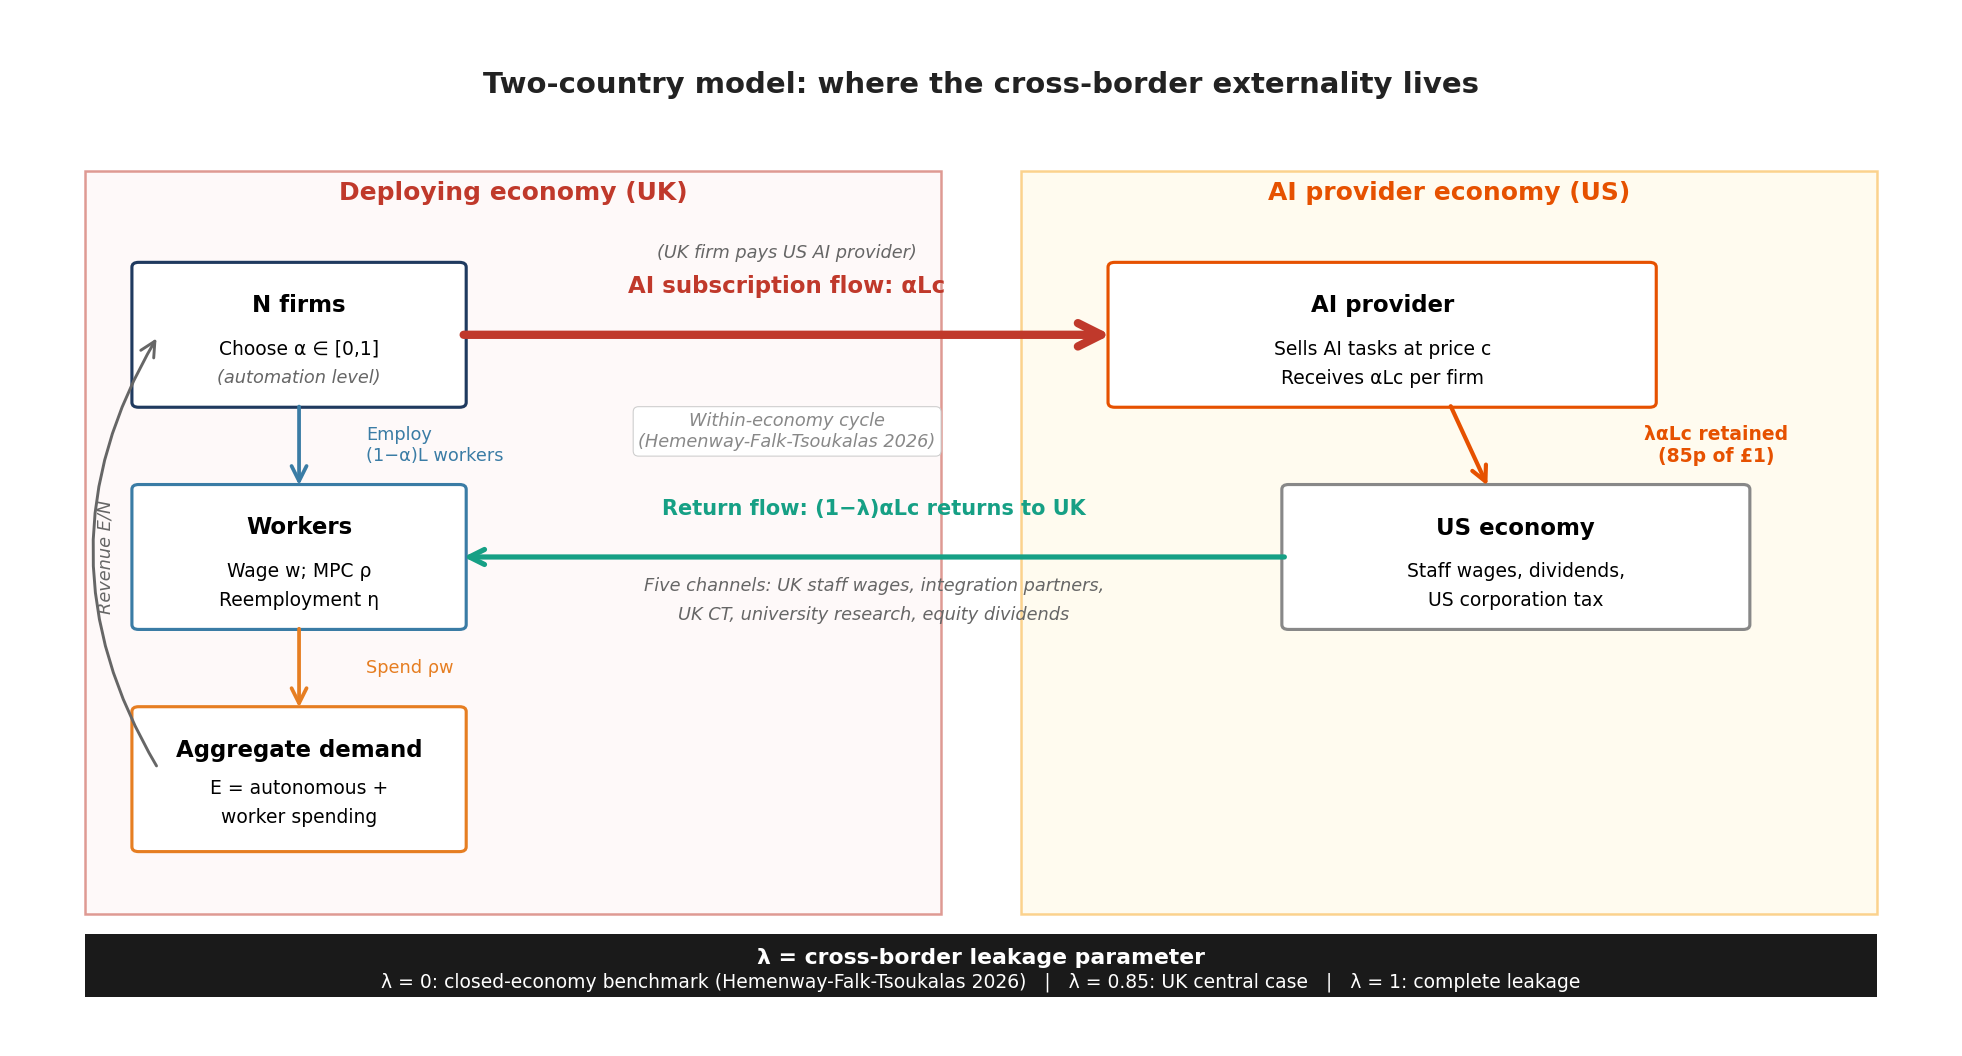
\includegraphics[width=0.95\linewidth]{figures/13_two_country_model.png}
\caption{Two-country model setup. The deploying economy (UK) hosts $N$ firms choosing automation $\alpha$, employing workers at wage $w$ with marginal propensity to consume $\rho$, generating aggregate demand $E$ that feeds back into firm revenue. The cross-border AI subscription flow $\alpha L c$ (red arrow) leaks to the AI provider economy (US). Of every \pounds 1 paid, fraction $(1 - \lambda)$ returns to the UK through five channels (green arrow): UK staff wages of US AI firms, integration partner margins, transfer-priced UK corporation tax, university research partnerships, and UK shareholder returns on US AI provider equity. Fraction $\lambda$ is retained in the US. At $\lambda = 0$ the model reduces to \citet{hemenway_falk_tsoukalas_2026}; at $\lambda = 0.85$ (UK central case) the cross-border externality dominates the within-economy externality.}
\label{fig:model}
\end{figure}

\subsection{Six Propositions}

\begin{proposition}[Closed-economy benchmark]\label{prop:closed}
When $\lambda = 0$, the model reduces to \citet{hemenway_falk_tsoukalas_2026}, and the optimal Pigouvian automation tax is $\tau^* = (1 - 1/N) \rho$.
\end{proposition}

\begin{proof_sketch}
Substituting $\lambda = 0$ into the demand equation produces full recirculation of {AI} payments, equivalent to the closed-economy benchmark. The Hemenway-Falk-Tsoukalas (2026) optimal-tax derivation applies unchanged.
\end{proof_sketch}

\begin{proposition}[Cross-border leakage strictly worsens the externality]\label{prop:lambda_worsens}
For any $\lambda > 0$, the social cost of automation exceeds the closed-economy social cost by an amount strictly increasing in $\lambda$.
\end{proposition}

\begin{proof_sketch}
The cross-border term in aggregate expenditure decreases monotonically in $\lambda$. By construction, lower aggregate expenditure produces lower equilibrium output and welfare, holding $\alpha$ fixed. The marginal social cost of automation is therefore strictly higher when $\lambda > 0$.
\end{proof_sketch}

\begin{proposition}[Domestic Pigouvian taxation is insufficient]\label{prop:domestic_insufficient}
For any $\lambda > 0$, no domestic automation tax $\tau$ can fully internalise the cross-border externality. The closed-economy optimal tax $\tau^* = (1 - 1/N) \rho$ leaves residual welfare loss strictly increasing in $\lambda$.
\end{proposition}

\begin{proof_sketch}
The closed-economy tax targets the demand externality from displaced wages. The cross-border externality operates through a separate channel: {AI} subscription payments leaving the economy. A tax on automation reduces both channels proportionally but cannot target the cross-border channel selectively. The residual cross-border welfare loss is irreducible under purely domestic taxation.
\end{proof_sketch}

\begin{proposition}[Complementary {DST} is required]\label{prop:dst}
Under cross-border leakage $\lambda > 0$, the welfare-optimising policy combines a domestic automation tax $\tau_a$ with a digital services tax $\tau_d$ on {AI} subscription revenue. With endogenous tax avoidance $\delta(\tau_d) = \delta_0 + \beta \tau_d$, the welfare-maximising {DST} rate is $\tau_d^* = (1 - \delta_0) / (2\beta)$.
\end{proposition}

\begin{proof_sketch}
DST revenue $R(\tau_d) = \tau_d \lambda (1 - \delta_0 - \beta \tau_d) S$ is concave in $\tau_d$ once avoidance is endogenous. The first-order condition gives the standard Laffer-curve maximum: above $\tau_d^*$ avoidance erodes the rate increase faster than the rate increase adds; below $\tau_d^*$ the reverse holds. Welfare-maximisation gives the same $\tau_d^*$ when captured revenue returns to UK households. Full derivation in Appendix~A.
\end{proof_sketch}

\begin{proposition}[Tax-instrument capture is bounded at UK parameters]\label{prop:infeasible}
At {UK} parameters ($\lambda \approx 0.85$, avoidance calibration $\delta_0 \approx 0.42$, $\beta \approx 1.67$), the optimal {DST} rate is approximately 17\% nominal, and the realised capture is approximately 4\% of gross AI subscription flow. Tax instruments alone cannot close the cross-border externality, not because the optimal rate is unattainable, but because realisable capture is mechanically bounded by avoidance.
\end{proposition}

\begin{proof_sketch}
Substituting UK parameters: $\tau_d^* = (1 - 0.42)/(2 \times 1.67) \approx 0.174$. At this rate, $\delta(\tau_d^*) \approx 0.71$, so realised capture $= \tau_d^* \times \lambda \times (1 - \delta) \approx 0.043$, or 4.3\% of gross flow. Applied to cumulative \pounds139 billion AI subscription flow through 2030, the DST captures approximately \pounds6 billion. The result is robust to $\beta \in [1.0, 2.5]$, with capture share remaining single-digit. Full numerical derivation in Appendix~A.
\end{proof_sketch}

\begin{proposition}[Industrial policy is welfare-necessary]\label{prop:industrial}
Under the parameter region of Proposition~\ref{prop:infeasible}, welfare improvement requires industrial policy that directly reduces $\lambda$ structurally rather than recapturing rent through taxation. The required interventions are: (i) demand-side capital allocation to domestic {AI} firms; (ii) supply-side infrastructure ownership reducing the leakage rate of allocated capital; and (iii) rent capture instruments at sustainable rates.
\end{proposition}

\begin{proof_sketch}
The structural reduction of $\lambda$ shifts the bargaining frontier between domestic firms and {AI} providers, reducing both the gross rent flow and the residual cross-border component. The three interventions are complementary rather than substitutable: capital allocation without infrastructure ownership produces high re-leakage rates; infrastructure ownership without capital allocation lacks domestic {AI} demand; both without rent capture leave the existing flow uncollected. Welfare maximisation requires all three.
\end{proof_sketch}

The full proofs and parameter sensitivities are developed in Appendix~A.

\section{The {UK} Empirical Setting}

\subsection{Magnitude and structure of {UK} {AI} adoption}

{UK} {AI} adoption has accelerated rapidly. The British Chambers of Commerce {AI} adoption module reports {UK} firm-level adoption at 23\% in 2023, 35\% in 2025, and projected 54\% in 2026 \citep{bcc_atos_2026}. Approximately 10\% of firms have moved beyond generic tools (ChatGPT, Copilot) into bespoke {AI} integration. Among bespoke adopters, approximately 20\% report staffing reductions attributable to {AI}, and bespoke adopters are roughly three times more likely to have restructured job roles than generic adopters.

The {UK} {AI} startup ecosystem is large by European standards. {UK} {AI} startups raised \pounds6 billion in venture capital in 2025, with more than \pounds3 billion in Q1 2026 alone---the second-highest concentration in Europe and approximately third globally after the {US} and China. Major {UK} {AI} firms include {DeepMind} (now wholly within Google), {Wayve} (autonomous driving, \$1 billion raised in 2024), {Synthesia} (synthetic media), {ElevenLabs} (voice {AI}), {Stability AI}, and {Stable AI}. The Alan Turing Institute and several Oxbridge research centres provide significant academic capacity.

\subsection{The displacement evidence}

The redundancy notice flow attributable to {AI}-driven restructuring across 2023--2026 is substantial. {HSBC} announced 20{,}000 cuts in March 2026, with the bank explicitly citing {AI} as a primary driver \citep{morgan_stanley_2026}. {KPMG} {UK} announced 590 cuts the same month, though with attribution language softer than {AI}-direct (the firm cited ``low attrition'' as the operational reason, contemporaneous with their {AI} transformation programme). The {BBC} announced Project Ada, a major {AI} restructuring programme, in late 2025. {BT} restated its 55{,}000-by-2030 reduction target with {AI} as the primary technology lever. {PwC} {UK} cut its 2025 graduate cohort by approximately 200 positions; {Deloitte} {UK} cut 800 positions plus 50{,}000 in India operations.

I aggregate these and similar announcements at sector level. Cumulative {UK} {AI}-attributable layoffs Q1~2023 through Q1~2026 reach approximately 62{,}400 at a 50\% attribution rate---meaning approximately half of the announced restructuring is treated as {AI}-driven, with the remainder attributable to other factors (cost pressures, regulatory change, normal business cycle). The 50\% attribution is conservative relative to {Morgan Stanley} (who treat their figures as {AI}-direct) and aggressive relative to firms like {KPMG} whose attribution language is softer than {AI}-direct.

\begin{figure}[ht]
\centering
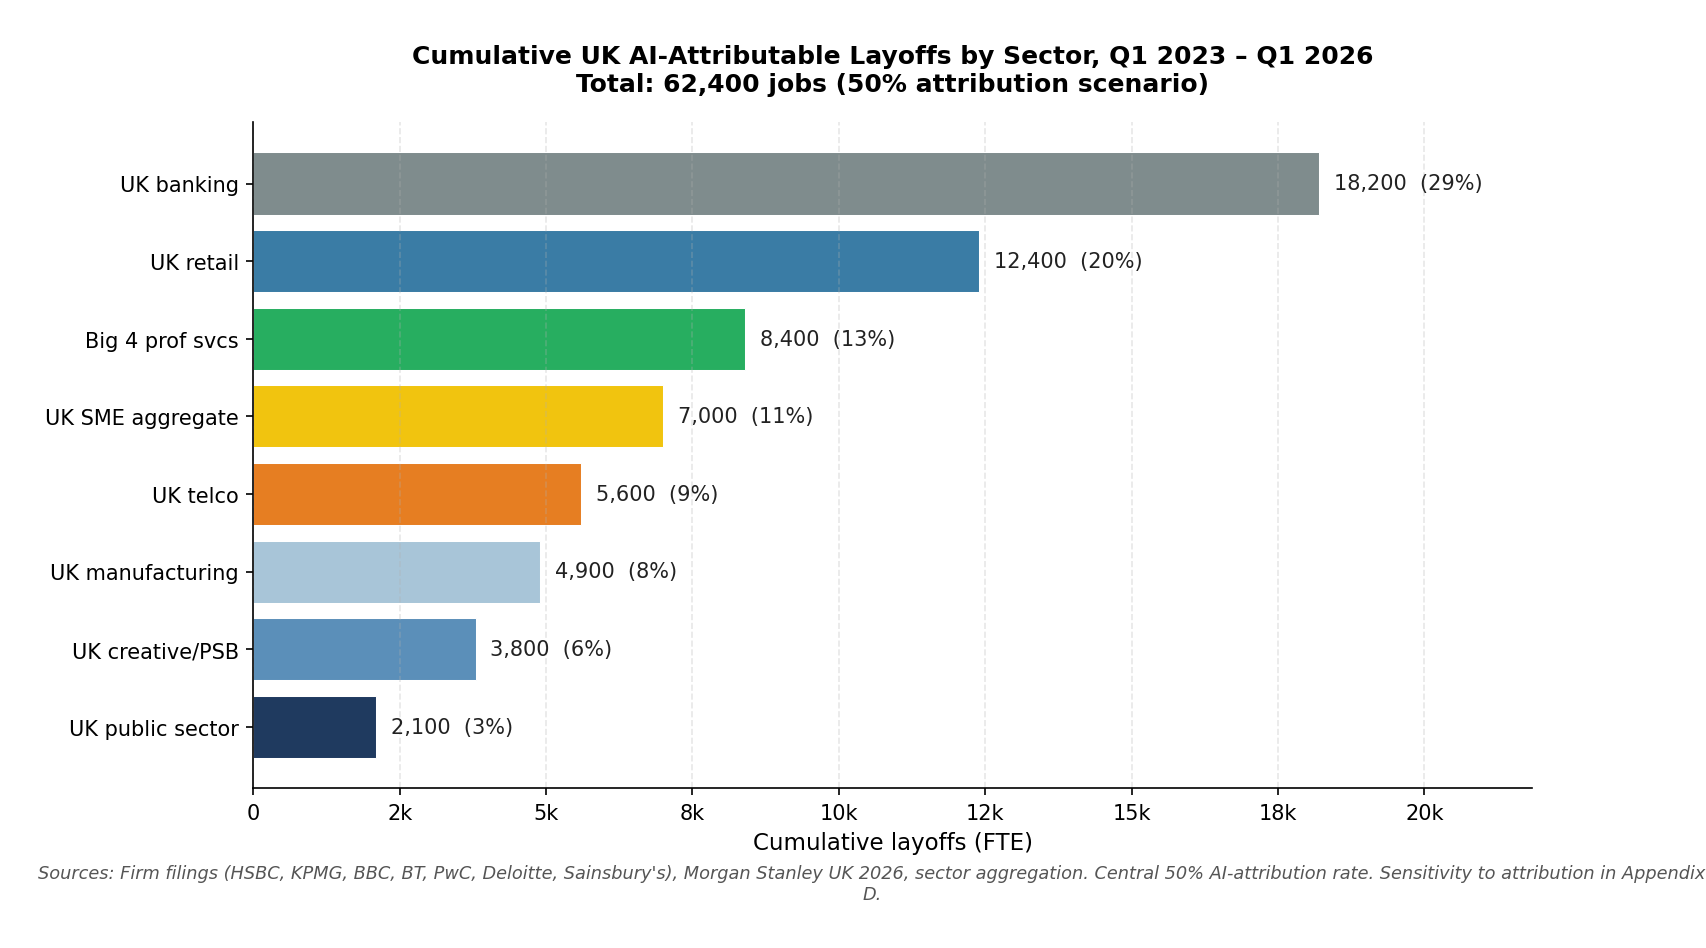
\includegraphics[width=0.85\linewidth]{figures/03_sectoral_displacement.png}
\caption{Cumulative UK AI-attributable layoffs by sector at 50\% attribution, Q1 2023 through Q1 2026. Banking, professional services, and retail account for the majority of visible displacement. The figure uses central attribution; sensitivity to attribution rate is documented in Appendix~D.}
\label{fig:sectoral}
\end{figure}

\subsection{The puzzle the data presents}

\citet{morgan_stanley_2026} reports that {UK} firms with at least one year of {AI} deployment record 8\% net {AI}-linked job loss against an international average of 4\%, despite achieving 11.5\% productivity gains identical to {US} firms which posted net job creation. This is the empirical anomaly. Same productivity gain, opposite employment outcome.

In a single-country framework, this is unexplained. There is no reason productivity gains should produce divergent employment outcomes across two economies with similar institutions, similar enterprise software stacks, and similar {AI} adoption rates. My framework provides the explanation. The cross-border rent flow recirculates within the {US} economy because {AI} providers are {US}-domiciled---wages, taxes, dividends, and shareholder returns flow back to {US} consumer demand. The same flow does not recirculate in the {UK} because {AI} providers are foreign---payments leave the country, are not absorbed by domestic firms, and reduce consumer demand in the deploying economy. The Hemenway-Falk-Tsoukalas demand externality compounds with the cross-border leakage, producing higher net displacement in the {UK} than in the {US}.

I do not rely on the {Morgan Stanley} figure as an empirical anchor for my calibration. My cross-border rent leakage parameter $\lambda$ is estimated independently from public-record data on Microsoft Ireland accounts, Companies House filings, and {ONS} trade statistics. I cite \citet{morgan_stanley_2026} as one piece of evidence consistent with my framework's predictions, alongside the Stargate {UK} natural experiment, the Microsoft Ireland transfer-pricing structure, and the cumulative {UK} redundancy notices.

\subsection{The {UK} macro context}

{UK} unemployment stands at 4.9\%, the highest rate since 2021 \citep{obr_2026}. Vacancies have fallen to 711{,}000---a five-year low. Payrolled employees decreased by 74{,}000 year-on-year to February 2026. {GDP} per capita fell in the second half of 2025. Real {GDP} grew 1.3\% in 2025 (since revised to 1.4\%), with more than half the growth attributable to public-sector spending while private-sector output growth was essentially flat. The Bank of England forecasts unemployment to remain elevated through 2027. The {UK} productivity environment over this period has been characterised by stagnation in headline output per worker alongside compositional shifts that include labour-shedding without commensurate capital deepening---a pattern consistent with displacement rather than reabsorption.

This context matters for the paper's framing. The {UK} is not in a labour-market environment where {AI} displacement is being absorbed by reabsorption into other sectors at scale. The aggregate evidence is more consistent with displacement persisting than with reabsorption operating efficiently.

\subsection{Engaging the {Anthropic Economic Index} {UK} labour market analysis}

A recent {UK} labour-market study using the {Anthropic Economic Index} \citep{british_progress_2026} reports that {AI}-exposed {UK} occupations have grown marginally faster than unexposed occupations since November 2022, suggesting that sectoral reallocation may be absorbing {AI}-driven displacement at the occupation level. I engage with this finding directly because it is the most significant published challenge to the displacement evidence on which my calibration depends.

The {AEI} measure is occupational headcount. This measure cannot identify five things that bear on the welfare arithmetic. First, headcount counts roles, not the same workers occupying them: a marketing executive made redundant and replaced by a prompt engineer hired from outside the occupation appears as zero net change in occupational headcount, masking the displacement entirely. Second, headcount does not weight by wage: a senior role made redundant and replaced by a junior role at a lower salary appears as zero net change, even though the wage bill, consumer demand, and tax revenue have all fallen. Third, the reskilling literature documents that displaced workers experience persistent earnings losses of 15--25\% over horizons of six to twenty years \citep{jacobson_lalonde_sullivan_1993}, which the {AEI}'s panel cannot capture. Fourth, the aggregate {UK} labour market is not consistent with broad-based reabsorption: unemployment stands at 4.9\%---the highest since 2021---vacancies have fallen to a five-year low, payrolled employees are down 74{,}000 year-on-year, and the ratio of unemployed people per vacancy has risen from 2.0 to 2.5 over the past year \citep{obr_2026}. Fifth, and most importantly for my purpose, the {AEI} measure does not capture cross-border rent flow at all. Reabsorption at the occupation level, even if it were occurring at the rate the {AEI} implies, would not heal the \pounds139 billion of subscription payments leaving the {UK} by 2030, the \pounds95 billion of cloud-for-{AI} flow, or the \pounds105 billion of productivity rent transferred to {US} shareholders. These are independent phenomena. This paper measures the rent flow; the {AEI} measures occupational headcount. The two findings could both be correct simultaneously and my central conclusion would stand.

\begin{figure}[ht]
\centering
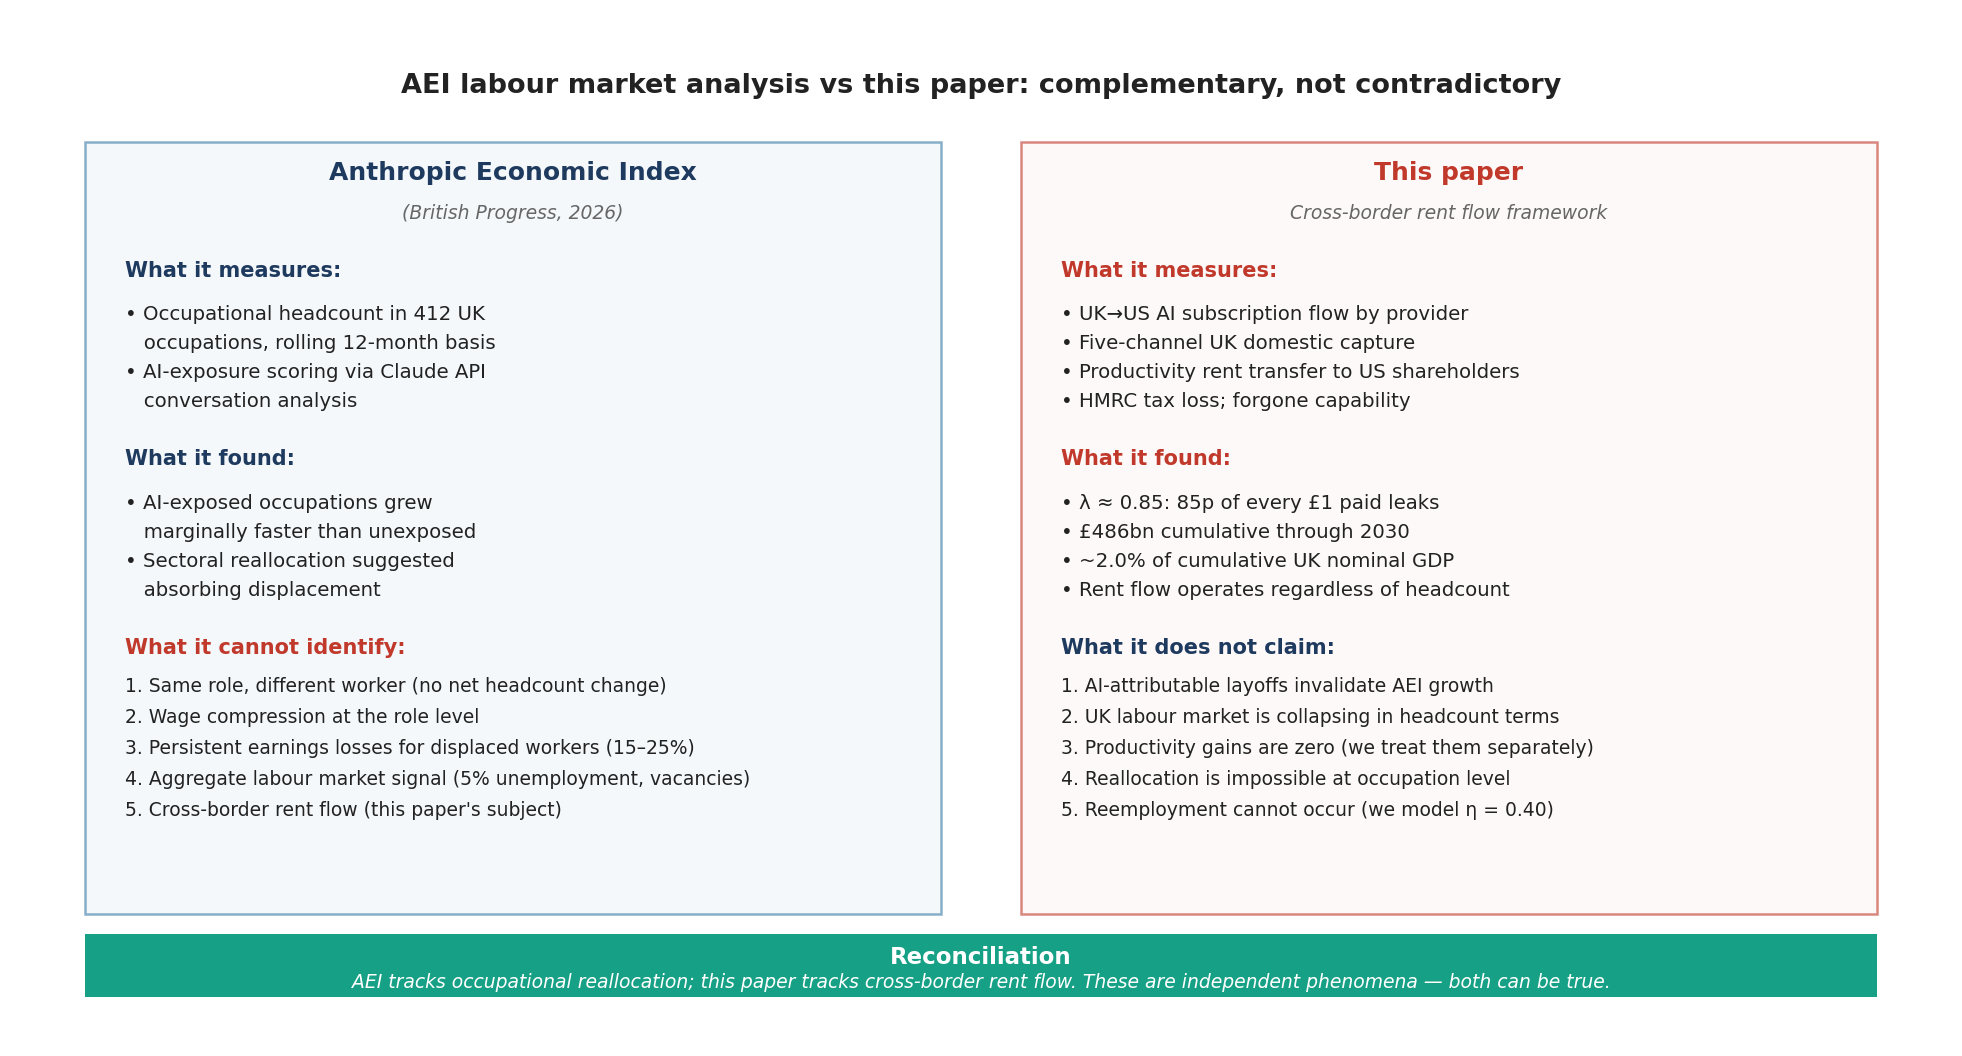
\includegraphics[width=0.95\linewidth]{figures/14_aei_comparison.png}
\caption{The Anthropic Economic Index (British Progress, 2026) and this paper measure different phenomena. AEI tracks occupational headcount and finds marginal positive growth in AI-exposed UK occupations. This paper tracks cross-border AI rent flow and finds \pounds461 billion cumulative through 2030. The findings are complementary, not contradictory: occupational reallocation does not heal the rent flow; the rent flow operates regardless of headcount.}
\label{fig:aei}
\end{figure}

\subsection{Triangulation across three independent sources}

The three available data sources point to the same underlying mechanism when interpreted at their appropriate scope. {Morgan Stanley} examines firms with at least one year of {AI} deployment---the early-adopter subset where {AI}-driven restructuring is most visible---and finds 8\% net job loss. The {AEI} examines all 412 {UK} occupational categories using rolling 12-month employment counts---the broader economy where reabsorption may operate at the margin---and finds marginal positive growth. My calibration estimates 62{,}400 cumulative {AI}-attributable layoffs at 50\% attribution---a middle ground between the two extremes. The three findings are reconcilable: early adopters bear the displacement, broader occupations show reabsorption at the margin, and the cross-border rent flow operates regardless of either, accumulating to \pounds461 billion through 2030.

\subsection{Why the rent extraction is structural: the four-layer architecture}

The cross-border leakage parameter $\lambda$ in my model is empirically a single number, but mechanically it is a composite. {AI} rent extraction operates at four sequential layers of the supply chain, each with its own margin structure and its own ownership concentration. Understanding the layered architecture matters because it determines what policy can do.

\textit{Layer 1: Semiconductor fabrication and design.} The {AI} accelerator landscape is undergoing rapid restructuring. NVIDIA crossed \$5 trillion market capitalisation in April 2026 on the strength of its {GPU} dominance in training, with datacenter gross margins of approximately 75--80\%. But hyperscaler custom silicon is now ramping at scale: Google's eighth-generation {TPU}s (training and inference variants, announced April 2026), Amazon's Trainium~3 and Trainium~4 (Anthropic committed \$100 billion over ten years to AWS Trainium silicon on 20 April 2026), Meta's MTIA family (four generations from MTIA~300 through MTIA~500 announced March 2026, with a 1{,}000~megawatt Broadcom partnership announced 14 April 2026), Microsoft's Maia~200, and OpenAI's custom chip with Broadcom expected in late 2026. The competitive dynamics are intra-{US}: NVIDIA versus Google versus Amazon versus Meta versus Microsoft versus OpenAI, with the residual to {AMD} and Intel. Semiconductor design is approximately 95\% {US}-controlled across this expanded set---more concentrated than under the previous NVIDIA-monopoly framing, not less, because the alternatives that have materialised at scale are also {US}-domiciled. Fabrication is concentrated in {TSMC} (Taiwan) and Samsung (Korea). This is the deepest moat in the {AI} stack and the one with the highest barrier to entry: a leading-edge fab costs \$20--30 billion; NVIDIA's annual {R\&D} budget is approximately \$15 billion; combined hyperscaler capex on {AI} infrastructure is approximately \$650 billion in 2026 alone.

\textit{Layer 2: Cloud infrastructure (IaaS).} {AWS}, Microsoft Azure, and Google Cloud Platform together hold approximately 65\% of global hyperscale cloud market share, with operating margins of 35--45\%. Capital expenditure at each of these firms is approximately \$80--100 billion per year, an order of magnitude beyond what any non-{US} firm currently deploys.

\textit{Layer 3: Foundation models.} OpenAI, Anthropic, Google, Meta, and xAI together control approximately 95\% of frontier foundation models. Training costs amortise across enterprise contracts at gross margins of 50--70\%. Sovereign foundation models exist in the {EU} (Mistral) and elsewhere but have not yet matched frontier capability at scale.

\textit{Layer 4: Applications (SaaS).} Microsoft Copilot, Salesforce Agentforce, ChatGPT Enterprise, and similar applications operate at 25--35\% gross margins. Application-layer firms are distributed across {US}, {UK}, {EU}, and {AU} jurisdictions; this is the only layer with meaningful local competition.

The {UK} Sovereign {AI} Fund, in its current scope, operates at Layer 4. It funds {UK}-based application companies. But every Layer 4 application runs on Layer 2 infrastructure ({AWS}/Azure {UK} regions), running Layer 3 models, executing on Layer 1 hardware. Of every pound deployed in a {UK} {AI} startup, approximately 55--70 pence flows back to {US} providers at Layers 1--2 through portfolio-company operating costs (Section~8.3). The structural rent extraction operates at the upstream layers regardless of where the downstream firm is domiciled, and---critically---regardless of which specific {US} firm captures it. When a {UK} firm pays for inference, the rent flow lands somewhere in the {US} tech ecosystem: NVIDIA if Blackwell {GPUs} run the workload, Amazon if Trainium runs it, Google if {TPU} runs it, Meta or Microsoft if their internal silicon runs it. Intra-{US} competition redistributes the capture; it does not reduce the leakage. The same logic applies to {US}-domiciled firms: when Uber spent its 2025 {AI} budget on {AI} compute and tooling, the rent flowed to whichever {US} provider won the contract, not to Uber's complementary workforce or to non-{US} alternatives. The Layer 1--2 monopoly drains everyone, {US} or otherwise, who builds {AI} applications at Layer 4---except that {US} consumer demand recirculates back to {US} firms, while {UK} consumer demand does not.

This has direct implications for the policy framework developed in Section~8. The three-pillar framework I propose is what the {UK} can do unilaterally: rent capture (Pillar~1), demand-side capital allocation at Layer 4 (Pillar~2), and supply-side leakage reduction through {UK}-hosted compute and energy policy (Pillar~3). Pillars 1--3 do not address the upstream Layer 1--2 monopoly directly, because no individual non-{US} economy has the capital scale to build alternatives at frontier. A full structural response to the Layer 1--2 monopoly would require multilateral coordination at scales that go beyond what this paper attempts to specify; I flag this as a frontier of future work rather than offer a specific proposal.

\begin{figure}[ht]
\centering
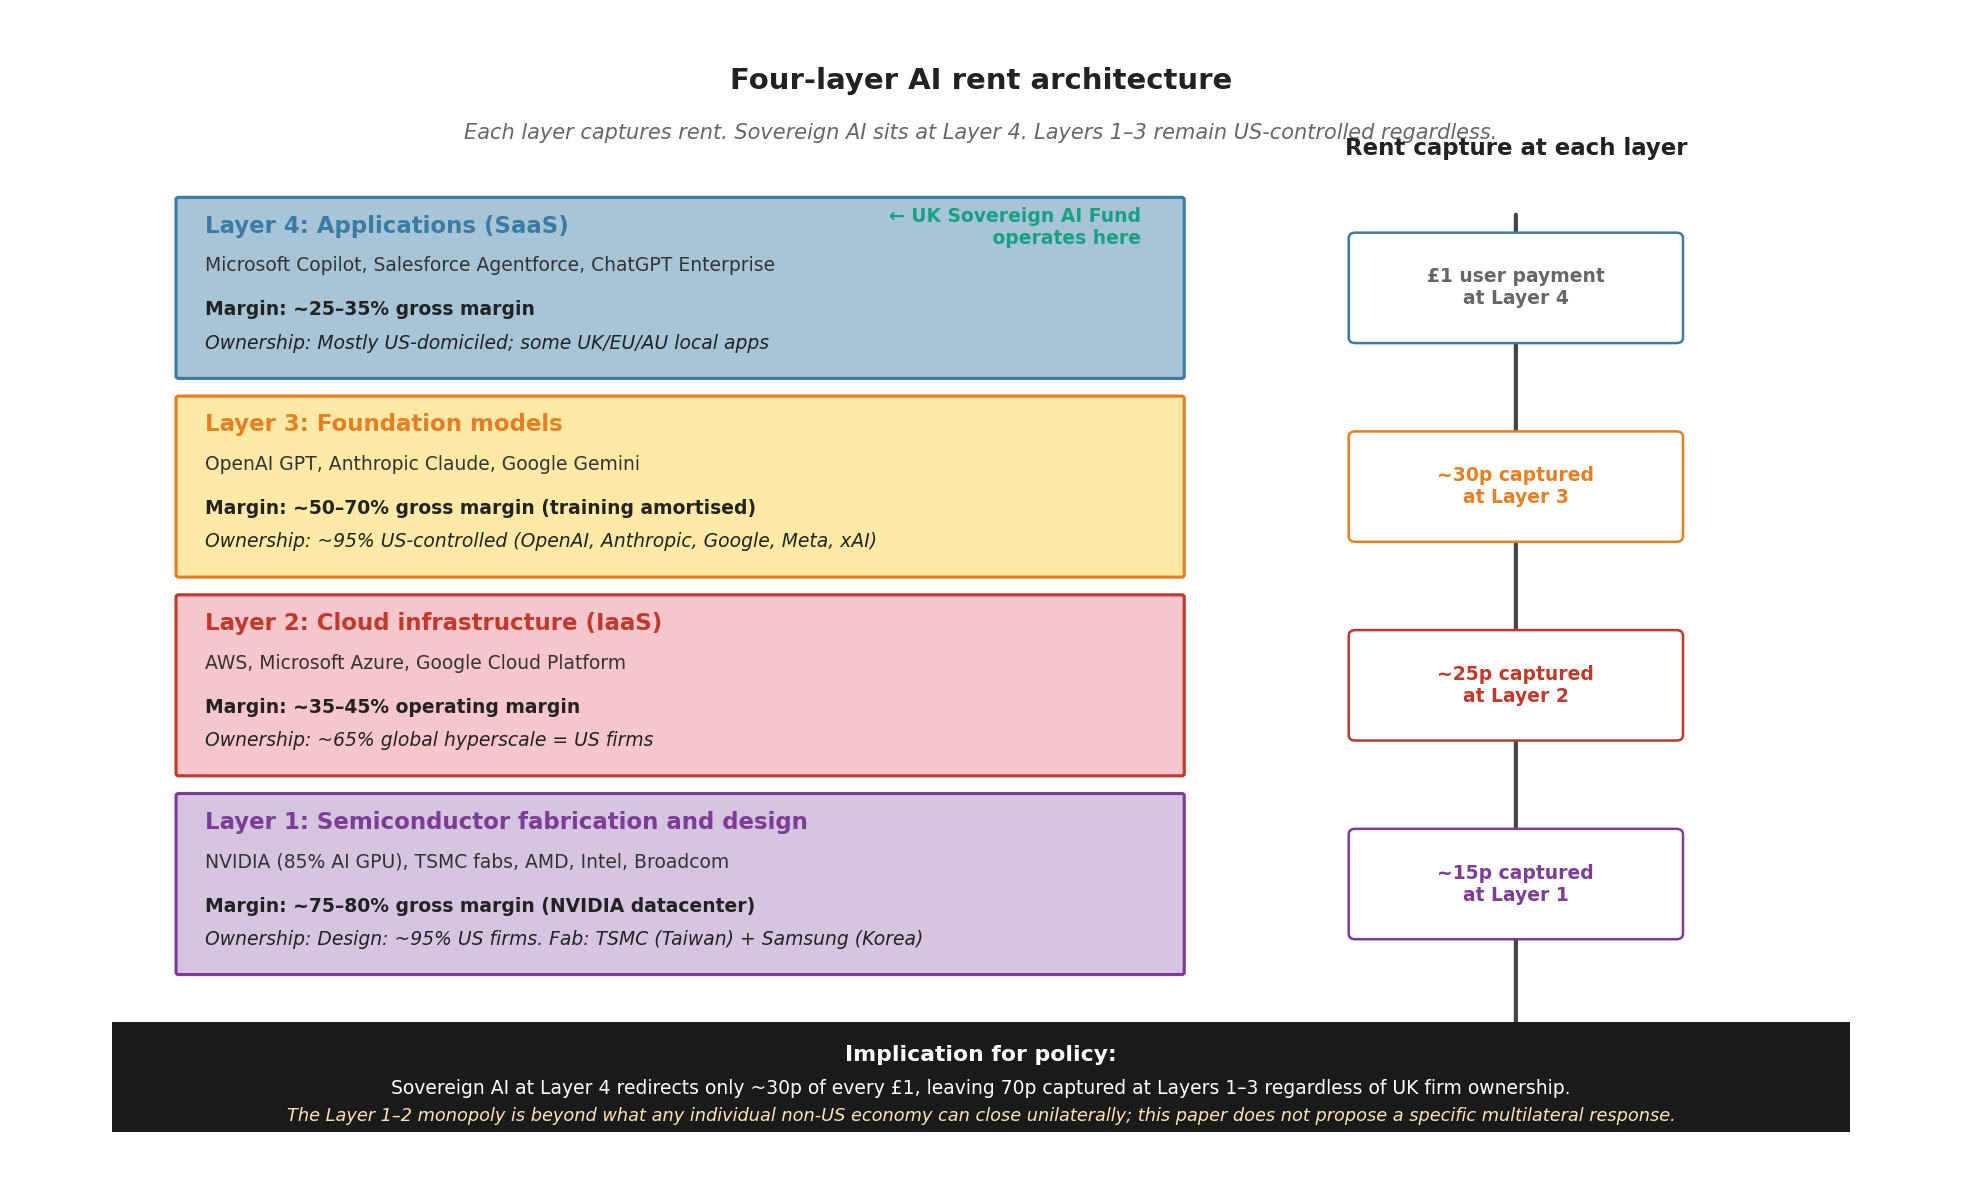
\includegraphics[width=0.95\linewidth]{figures/19_four_layer_rent.png}
\caption{Four-layer AI rent architecture. Each layer captures rent at its margin structure, with concentration of US ownership rising as one moves down toward the foundation. The UK Sovereign AI Fund operates at Layer 4; Layers 1--3 are not addressed by the three-pillar framework I propose, because the capital scale required exceeds what any individual non-US economy can deploy unilaterally. Margin and ownership figures from firm 10-K filings, IDC Worldwide Public Cloud Services Tracker, IFR World Robotics, NVIDIA financial reports.}
\label{fig:fourlayer}
\end{figure}

\begin{figure}[ht]
\centering
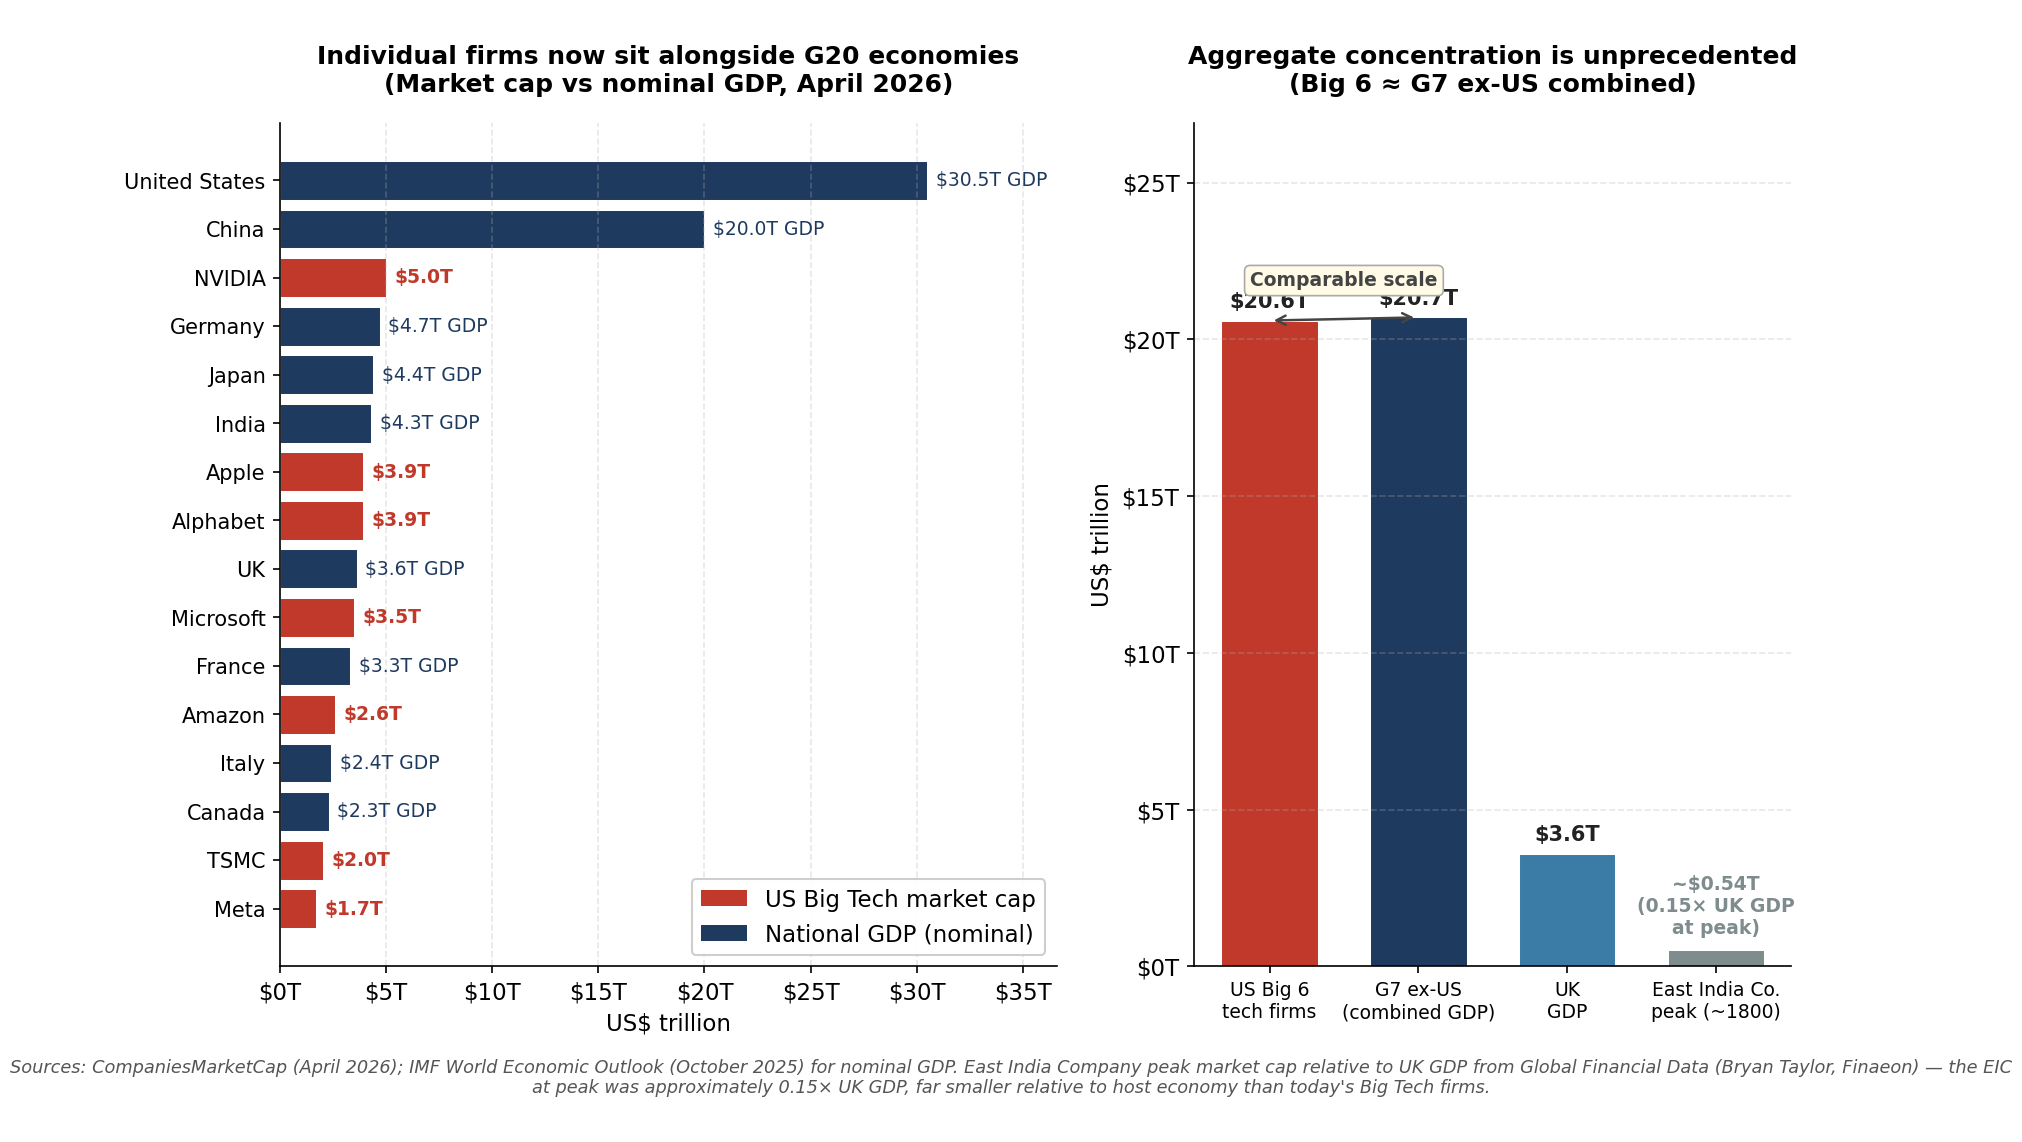
\includegraphics[width=0.95\linewidth]{figures/18_marketcap_vs_gdp.png}
\caption{The structural backdrop: private capital concentration relative to nation-state economies. Left panel: top US Big Tech firms ranked alongside major economies' nominal GDP, April 2026. NVIDIA at \$5.0 trillion (post 24~April 2026) exceeds the GDP of every economy except the US and China. Right panel: aggregate Big Six US tech firms (\$21 trillion) approximate the combined nominal GDP of the G7 excluding the US (\$20.7 trillion). The East India Company at peak around 1800 was approximately 0.15$\times$ UK GDP, an order of magnitude smaller relative to host economy.}
\label{fig:marketcap}
\end{figure}

\subsection{The custom-silicon shift sharpens the cross-border argument}

In the weeks immediately preceding this draft (March--April 2026), the structure of the {AI} accelerator market changed materially. On 11 March, Meta announced four successive generations of its in-house Meta Training and Inference Accelerator ({MTIA}~300, 400, 450, 500), with deployment cadence of one new chip every six months and a stated goal of running ranking, recommendation, and {GenAI} inference workloads on internal silicon. On 14 April, Broadcom and Meta announced an extended partnership through 2029 with Meta deploying over 1{,}000 megawatts of custom {MTIA} silicon initially, scaling to multi-gigawatt rollout. On 20 April, Anthropic committed more than \$100 billion over ten years to {AWS} Trainium and Graviton silicon, securing up to 5{,}000 megawatts of capacity for training and serving Claude---the company that produced the dominant frontier model used by enterprise customers no longer plans to run that model on NVIDIA hardware. On 22 April, Google announced its eighth-generation {TPU}s ({TPU}~8t for training, {TPU}~8i for inference), with a single superpod scaling to 9{,}600 chips and 121 exaflops of compute. Microsoft's Maia~200 (TSMC 3nm, 216~GB HBM3e) and OpenAI's custom chip with Broadcom (expected late 2026) round out the picture. Industry analysis projects custom {AI} chip revenue growth of approximately 45\% in 2026 against {GPU} growth of approximately 16\%.

The naive reading of this development is that NVIDIA's monopoly is fracturing and the upstream {AI} rent extraction will weaken. That reading is wrong. The companies that have materialised at scale to compete with NVIDIA at Layer~1 are Google, Amazon, Meta, Microsoft, and OpenAI---all {US}-domiciled. The companies competing at Layer~2 are the same three hyperscalers that controlled Layer~2 before ({AWS}, Azure, Google Cloud), now with the additional advantage of vertical integration into their own silicon supply. The {UK} firm that pays for {AI} inference in 2026 has more counterparties than it had in 2024, but every counterparty in the inference market that operates at scale is {US}-domiciled. Intra-{US} competition redistributes which {US} firm captures the rent; it does not reduce the leakage parameter $\lambda$.

The custom-silicon shift therefore strengthens rather than weakens the argument of this paper. It removes the most sympathetic counterfactual under which $\lambda$ might mean-revert: a hypothetical world in which non-{US} {GPU} alternatives (Cerebras, Graphcore, Tenstorrent, {SambaNova}, or alternative national champions) achieved frontier-comparable performance and competed against NVIDIA on price. That counterfactual is now substantially less plausible. Any alternative-chip strategy aiming to compete at Layer~1 is not competing only against NVIDIA's roadmap; it is competing against NVIDIA \textit{plus} Google's {TPU} roadmap \textit{plus} Amazon's Trainium roadmap \textit{plus} Meta's {MTIA} roadmap \textit{plus} Microsoft's Maia roadmap \textit{plus} OpenAI's Broadcom-fabricated custom silicon. The competitive frontier for non-{US} entrants has hardened materially.

This has two implications for the {UK} policy framework. First, Pillar~3 (supply-side infrastructure ownership, Section~8.3) faces a harder competitive landscape than it did 18~months ago. Partnerships with Cerebras, Graphcore, or Tenstorrent will not produce alternatives at the scale or specialisation of hyperscaler-internal silicon. The {UK}-hosted compute capacity proposed in Pillar~3 will have to compete on cost-per-inference against {AWS} Trainium, Google {TPU}, Meta {MTIA}, and Microsoft Maia simultaneously, not just against NVIDIA pricing. Second, and more importantly, the analytical case for treating $\lambda$ as structural rather than cyclical has been strengthened by direct empirical evidence. The {US} dominance of frontier {AI} infrastructure is not contingent on a single firm's monopoly position; it is distributed across at least six {US}-domiciled firms with combined market capitalisation exceeding \$15 trillion and combined 2026 capital expenditure on {AI} infrastructure of approximately \$650 billion. No non-{US} economy or coalition can outspend that capex envelope at the relevant horizons.

The productivity rent capture trajectory in Component~3 (5\% rising to 32\% by 2030, Section~7.1) merits reconsideration in light of intra-{US} competition. The original calibration anchored on the cloud computing precedent ({AWS}, Azure, Google Cloud captured 25--35\% of customer surplus over 2010--2025) under near-monopoly pricing dynamics. Intra-{US} competition between five hyperscaler silicon programmes plus NVIDIA may compress the achievable capture rate at the margin, plausibly to 20--25\% rather than 32\% by 2030. I flag this as a downside risk to the Component~3 estimate but do not revise the central case, because (i) the price competition operates among providers that are all capturing rent from non-{US} customers regardless of which provider wins the contract, and (ii) the empirical evidence from 2026 ({Microsoft Copilot} December~2025 13\% price increase, {Salesforce} Agentforce token-based pricing transition) is consistent with rising rather than compressing {AI} provider pricing power.

\section{Estimating $\lambda$ for the United Kingdom}

This section estimates the cross-border rent leakage parameter $\lambda$ for the {UK}. The estimation has two parts. First, I measure the gross {UK}-to-{US} {AI} subscription flow. Second, I decompose {UK} domestic capture from {US} {AI} provider revenue into five channels and compute each from public data. The implied $\lambda$ is one minus the ratio of total domestic capture to gross flow.

\subsection{Gross flow estimation}

I construct seven provider-level series from 2023 to 2027: Microsoft (Copilot Enterprise plus Azure OpenAI), OpenAI direct ({API} plus Enterprise), Salesforce (Agentforce plus Einstein), Google (Workspace {AI} plus Vertex), {AWS} (Bedrock plus {AI} services), Anthropic (Claude Enterprise), and an aggregate ``other {US}'' category covering Oracle, CoreWeave, Scale {AI}, and smaller suppliers.

Each series is built bottom-up from {UK} penetration rates, average effective seat prices, and {UK} total addressable seats by sector. Aggregating across providers, gross {UK}-to-{US} {AI} subscription flow is \pounds1.86 billion in 2023, \pounds4.30 billion in 2024, \pounds7.99 billion in 2025, \pounds13.30 billion in 2026, and \pounds19.42 billion in 2027. Cumulative 2023--2027: \pounds46.9 billion. The extrapolation to 2030 assumes the year-on-year growth factor continues to decelerate from the 1.46$\times$ observed for 2026--27, dropping to approximately 1.30$\times$ in 2028, 1.20$\times$ in 2029, and 1.15$\times$ in 2030 as {UK} enterprise {AI} adoption approaches saturation. This deceleration produces 2028--2030 flows of approximately \pounds25, \pounds30, and \pounds35 billion respectively, giving cumulative 2023--2030 of approximately \pounds139 billion. A constant-1.46$\times$ geometric extrapolation would give \pounds177 billion instead; the deceleration assumption is empirically motivated by the typical S-curve of enterprise software adoption \citep{bcc_atos_2026} and by Microsoft and Salesforce's own 2026 guidance toward slower seat-count growth in mature markets.

I benchmark these against three independent series. First, {ONS} Pink Book Table 9.4 reports {UK} services imports from the United States at \pounds61.2 billion in 2024 \citep{ons_2024}. My estimated gross {AI} flow of \pounds4.3 billion is approximately 7\% of total {UK}-to-{US} services imports, rising to 13\% by 2025---consistent with published Gartner {UK} forecasts placing {AI}-attributable services at 15--20\% of {UK} enterprise software spend by 2025. Second, the published accounts of Microsoft Ireland Operations Limited (FY2025: \$93.1 billion revenue, \$5.2 billion pretax profit, {CRO} 16847294) imply Microsoft {UK} customer revenue of approximately \$7--8 billion, consistent with my Microsoft series. Third, the OpenAI International revenue figures imply {UK} share of approximately 12\%, consistent with my OpenAI direct figure for 2025.

Sensitivity bands are $\pm$25\% reflecting uncertainty in penetration rates and {AI}-attributable shares of generic cloud spend.

\begin{figure}[ht]
\centering
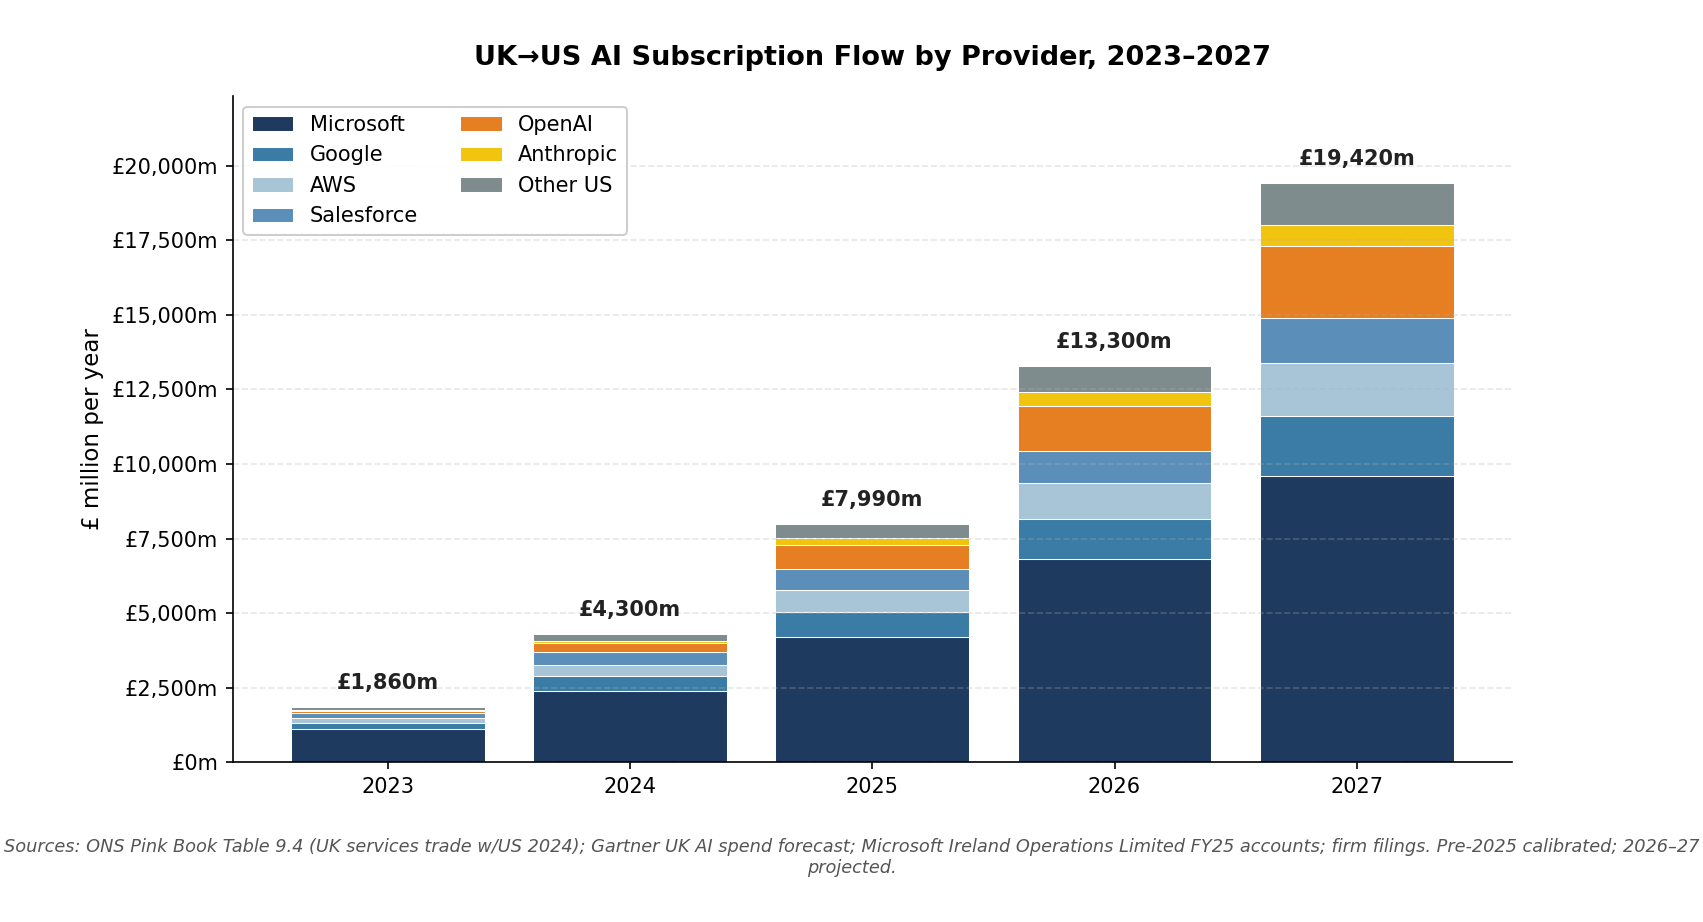
\includegraphics[width=0.85\linewidth]{figures/01_uk_us_ai_flow.png}
\caption{UK-to-US AI subscription flow by provider, 2023--2027. Microsoft accounts for nearly half. Pre-2026 figures are calibrated from public-record data; 2026--27 are projected from observed adoption rates.}
\label{fig:uk_us_flows}
\end{figure}

\subsection{The five channels of {UK} domestic capture}

\textbf{Channel 1: {US} {AI} firms' {UK} staff wages, weighted by {AI}-attributable share.} Microsoft {UK} (registered 01624297, approximately 7{,}500 staff in 2025), Google {UK} (approximately 5{,}000), {AWS} {UK} (approximately 3{,}000), Salesforce {UK} (approximately 3{,}000), Oracle {UK} (approximately 2{,}000), Anthropic {UK} (approximately 200), OpenAI {UK} (approximately 100), and smaller suppliers (approximately 1{,}000). Aggregate {UK} staff approximately 20{,}000. Loaded compensation \pounds85{,}000 average, total wage bill \pounds1.7 billion. {AI}-attributable share 33\%, anchored on Microsoft group reporting suggesting {AI} is approximately 25\% of revenue and rising.

\textbf{Channel 2: {UK} integration partner margins.} Nscale, Capita, Computacenter, Softcat, Bytes Technology, Phoenix Software resell {US} {AI} services at 5--8\% margins. Total {UK} integration partner {AI} revenue approximately \pounds3.5 billion in 2024 rising to \pounds7 billion in 2026. Average margin 6\%.

\textbf{Channel 3: Transfer-priced {UK} corporation tax.} Microsoft {UK} Ltd, Google {UK} Ltd, Amazon {UK} Services Ltd file Companies House accounts showing compressed margins consistent with transfer-pricing practice documented by \citet{torslov_wier_zucman_2018, torslov_wier_zucman_2023} and \citet{bilicka_2019}. Total {UK}-domiciled {AI}-attributable profit approximately \pounds450 million annually, generating corporation tax of approximately \pounds110--240 million across 2024--2026.

\textbf{Channel 4: {UK} university research partnerships.} Microsoft Research Cambridge, DeepMind {UK}, Anthropic London, OpenAI London spend approximately \pounds580 million annually in {UK} research. Direct {UK} research share approximately 55\%. {AI}-attributable share of direct portion approximately 60\%.

\textbf{Channel 5: {UK} equity holdings of {US} {AI} providers.} {UK} pension funds hold approximately \pounds105 billion of {US} Big Tech equity; {ISA}s approximately \pounds30 billion; {SIPPs} and direct retail holdings approximately \pounds40 billion. Total approximately \pounds175 billion against {US} Big Tech market capitalisation of approximately \pounds12 trillion ($\approx 1.5\%$ {UK} ownership share). The fraction returning to {UK} households via dividends and capital gains is approximately 0.9\% of provider gross flow, plus approximately 0.18\% via {HMRC} dividend and {CGT}.

\subsection{Implied $\lambda$}

\begin{table}[h]
\centering
\caption{Five-channel decomposition of {UK} domestic capture}
\begin{tabular}{cccccccc}
\toprule
Year & Gross Flow (\pounds m) & C1 & C2 & C3 & C4 & C5 & Total Capture (\pounds m) \\
\midrule
2024 & 4{,}300 & 540 & 180 & 110 & 180 & 40 & 1{,}050 \\
2025 & 7{,}990 & 605 & 280 & 165 & 215 & 74 & 1{,}339 \\
2026 & 13{,}300 & 680 & 410 & 240 & 240 & 120 & 1{,}690 \\
\bottomrule
\end{tabular}
\end{table}

The implied $\lambda$ is 0.756 in 2024, 0.832 in 2025, and 0.873 in 2026. The trajectory is rising because gross {AI} flow grows faster than the {UK} domestic {AI} ecosystem can absorb. Microsoft's {UK} staff has grown approximately 5\% per year while {UK} Copilot revenue has grown 90\% per year. The capture channels are constrained by physical {UK} {AI} ecosystem capacity; the gross flow is constrained only by {UK} enterprise willingness to adopt.

I use 0.85 as the central case for the model, midway between the 2025 value (0.83) and the 2026 value (0.87). The sensitivity range is $[0.78, 0.90]$. The point estimate is robust to several alternative parameterisations developed in Appendix~B.

\begin{figure}[ht]
\centering
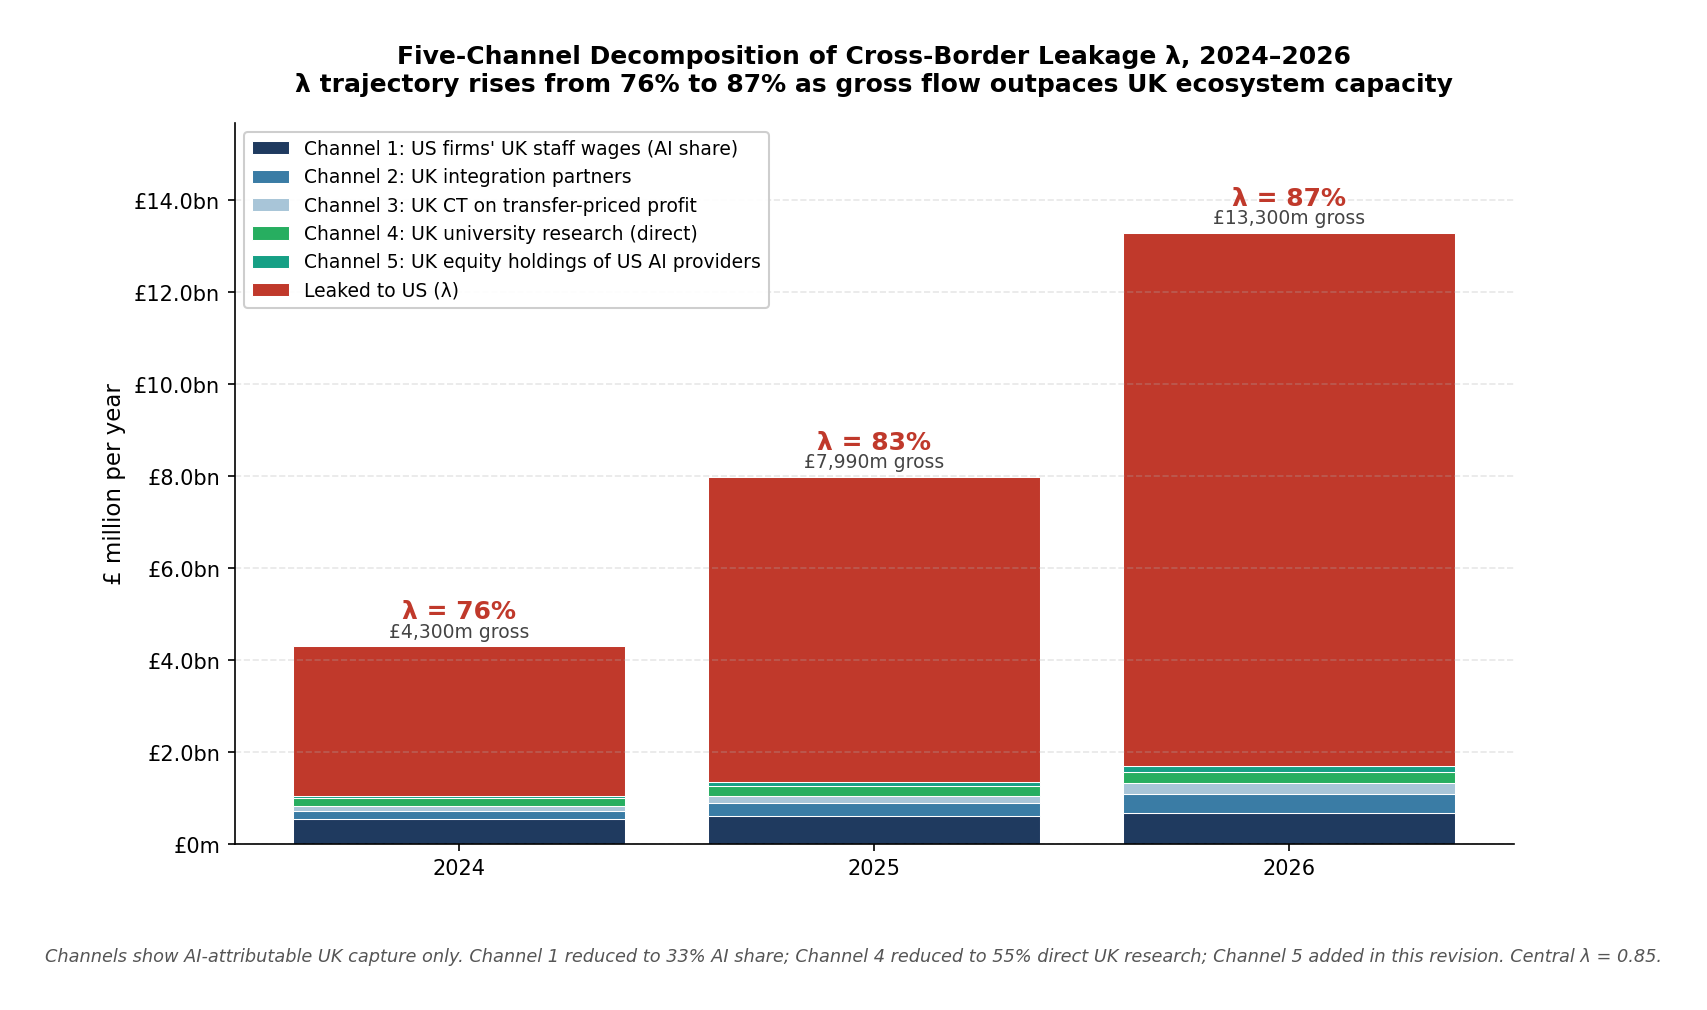
\includegraphics[width=0.85\linewidth]{figures/02_lambda_decomposition.png}
\caption{Five-channel decomposition of UK domestic capture, 2024--2026. Channel sizes show that approximately 13--24\% of gross UK-to-US AI subscription flow is captured domestically; the remaining 76--87\% is permanently extraterritorial. Channel 5 (UK equity holdings of US AI providers) is small in absolute terms but methodologically important to include.}
\label{fig:lambda_decomp}
\end{figure}

\subsection{Bilateral flows the paper does not measure}

I measure {UK}-to-{US} {AI} subscription flow and the cross-border leakage. The full {UK}-{US} bilateral economic relationship includes flows I do not measure. {US}-to-{UK} venture capital investment in {AI} startups was approximately \pounds8 billion cumulative through 2025. {US}-to-{UK} research grants and university partnerships are partially captured in Channel~4. {UK}-to-{US} talent migration to {US} {AI} firms with remitted income is estimated at \pounds2--3 billion annually. Tourism and other secondary effects exist but are small relative to the rent flow I identify. This paper isolates the {UK}-to-{US} {AI} subscription leak because it is the largest and most policy-actionable; I do not claim it is the only flow in the bilateral relationship.

\section{Stargate {UK} as a Natural Experiment}

The Stargate {UK} pause provides a natural experiment in cross-border {AI} deployment economics. Most analysis runs into a classic identification problem: deployment decisions are endogenous to the conditions that motivate them. Stargate {UK} is unusual because OpenAI publicly named the conditions required to revive the project. I can price them.

\subsection{The experimental structure}

On 17 September 2025, OpenAI, NVIDIA, and Nscale announced Stargate {UK} during the {US} president's state visit to Britain. The project specified deployment of 8{,}000 NVIDIA {GPUs} in Q1~2026, scalable to 31{,}000, across two North East sites: Cobalt Park in North Tyneside and Blyth in Northumberland. The {UK} government claimed \pounds30 billion in regional value and 5{,}000 jobs.

On 9 April 2026, OpenAI confirmed the project was paused. The publicly stated reasons were specific: {UK} industrial electricity at four times the {US} level (\pounds180 per {MWh} versus \pounds40 per {MWh} at large-user rates) and unresolved {AI} copyright regulation \citep{iea_2026}. OpenAI's statement: the company would ``continue to explore Stargate {UK} and will move forward when the right conditions such as regulation and the cost of energy enable long-term infrastructure investment.''

In parallel, several counterfactuals proceeded. {US} Stargate continued at \$500 billion announced scale. Stargate Norway proceeded with 100{,}000 NVIDIA {GPUs} and 230 megawatts at Narvik, drawing on Norwegian hydropower at approximately \pounds35 per {MWh}.

\subsection{The concession bundle}

OpenAI's stated conditions identify the regulatory and economic concessions required. I price each:

Energy subsidy: \pounds2.0--2.5 billion (matching {UK} large-user rates to {US} Texas levels for 250--300 {MW} over 10-year project life).

Text-and-data-mining ({TDM}) exception: \pounds15--22 billion present value. The {UK} creative industries' {AI}-vulnerable subsegment is approximately \pounds40--60 billion in gross value added (music, publishing, certain visual arts), narrower than the full {DCMS} \pounds125 billion creative industries figure. At 1\% perpetual licensing equivalent, discounted at 4\%, present value is \pounds15--22 billion.

Weakened {AISI} pre-deployment testing: \pounds4--6 billion (reduced compliance costs and faster deployment timelines).

Statutory liability shielding: \pounds5--8 billion (reduced {UK} litigation exposure).

Public-procurement preferences: \pounds2--4 billion.

{GDPR} Article 22 softening: \pounds3--5 billion (reduced compliance costs across regulated sectors).

\textbf{Total concession bundle: \pounds31--47 billion.}

\subsection{Project value to the {UK}}

Construction-phase value-add: \pounds1.0--1.5 billion (30--40\% domestic retention on \pounds3.2 billion build over 18--24 months).

Marginal $\lambda$ reduction for OpenAI specifically: \pounds2.0--3.0 billion {PV} (200--400 ongoing operational roles representing approximately 0.5\% reduction in {UK} OpenAI-specific $\lambda$).

Regional employment multipliers: \pounds0.5--1.0 billion {PV} (200--400 direct plus 600 indirect jobs).

Sovereign compute access: \pounds0.0--0.5 billion {PV} (marginal value of {UK}-resident versus {US}-resident compute under existing {OpenAI}-{UK} memorandum of understanding).

\textbf{Total project value to {UK}: \pounds4--5 billion {PV}.}

\subsection{The welfare arithmetic}

Welfare margin (pause superior to revival):
\begin{itemize}
\item Low cost minus high benefit: $\pounds31\text{bn} - \pounds5\text{bn} = \pounds26\text{bn}$
\item High cost minus low benefit: $\pounds47\text{bn} - \pounds4\text{bn} = \pounds43\text{bn}$
\end{itemize}

\textbf{Pause beats revival by \pounds26--44 billion.} For every pound of project value Stargate {UK} would deliver to the {UK}, it would cost approximately \pounds6--12 in concessions to make the project economically viable from OpenAI's perspective.

\begin{figure}[ht]
\centering
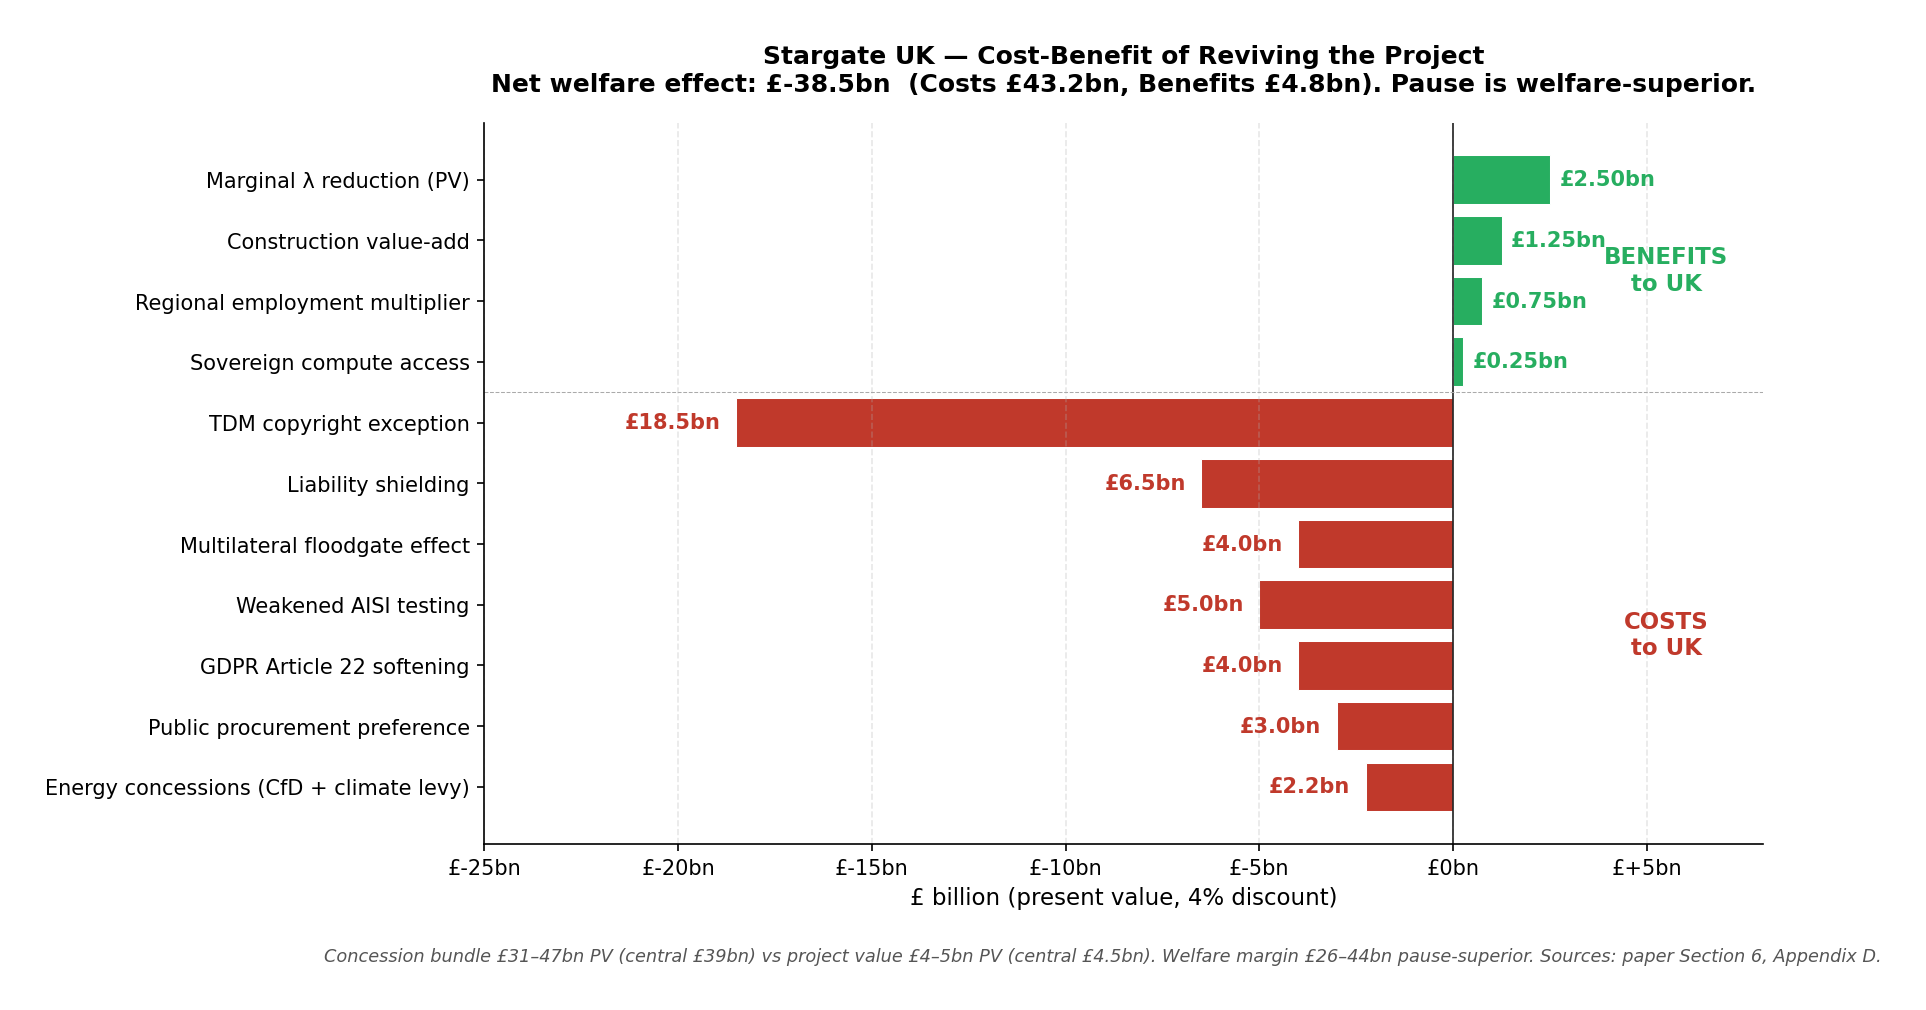
\includegraphics[width=0.85\linewidth]{figures/06_stargate_welfare.png}
\caption{Stargate UK welfare arithmetic. The concession bundle OpenAI requires to revive the project is worth \pounds31--47 billion in present-value cost to the UK, against project value of \pounds4--5 billion. The pause is welfare-superior by \pounds26--44 billion.}
\label{fig:stargate}
\end{figure}

\subsection{Why the regulatory channel is uniquely dangerous}

A {TDM} exception once granted applies to all {AI} providers globally, not only OpenAI. The concession is non-rivalrous and perpetual. $\lambda$ for OpenAI specifically might fall slightly with Stargate {UK} operational; but $\lambda$ for the broader {AI} provider universe rises because value previously captured by {UK} rights-holders is extracted by all {AI} providers including those without {UK} operational presence. An energy subsidy is reversible; a {TDM} exception is not.

\subsection{The generalisable bargaining structure}

A frontier {AI} provider has three margins of choice: deploy at home (highest expected return), deploy in a comparable non-frontier market with cheap energy and accommodating regulation (Norway, Texas, Wisconsin, Abu Dhabi), or deploy in a strategically-valuable but economically-marginal market that requires concessions to make viable (the {UK}, France, Germany).

The provider's reservation price for category-three deployments is the marginal value of category-two minus the additional cost of category-three. This reservation price is typically high enough to require concessions exceeding the direct project value. The non-frontier jurisdiction's reservation price is the value of the deployment minus the cost of the concessions. The bargaining range is empty: no concession bundle the provider would accept that the non-frontier jurisdiction should rationally offer.

The implication for {UK} policy is that competing for frontier {AI} infrastructure through concessions is structurally unprofitable. This does not mean {AI} infrastructure should not exist in the {UK}. It means it should be domestically-financed through the policy framework of Section~8 rather than concession-financed through inward-investment competition.

\subsection{Why Norway hosts and the {UK} cannot}

Norway is not in the same structural position as the {UK}. Norway has two flows running in opposite directions on the {AI} bilateral relationship.

Flow~A is {AI} consumption. Norwegian businesses buy Microsoft, OpenAI, and Salesforce subscriptions, exactly as {UK} businesses do. Norwegian $\lambda$ on this flow is in the same range as the {UK} ($0.80$--$0.85$). Norwegian businesses are getting drained by {US} {AI} providers in the same way British businesses are.

Flow~B is {AI} infrastructure hosting. Stargate Norway is OpenAI paying Norway for energy, land, construction labour, operational employment, and Norwegian corporation tax. Norway is selling commodity inputs (electricity, real estate, skilled construction) to a {US} {AI} buyer. Norwegian $\lambda$ on this flow is approximately $0.40$--$0.50$---most of the spend lands in Norway. This is an inflow from the {US} to Norway, partially offsetting Flow~A.

The {UK} has Flow~A at full magnitude. The {UK} does not have Flow~B. UK policymakers tried to bid for Flow~B with Stargate {UK} and lost the bid because {UK} industrial electricity is four times Norwegian.

\begin{figure}[ht]
\centering
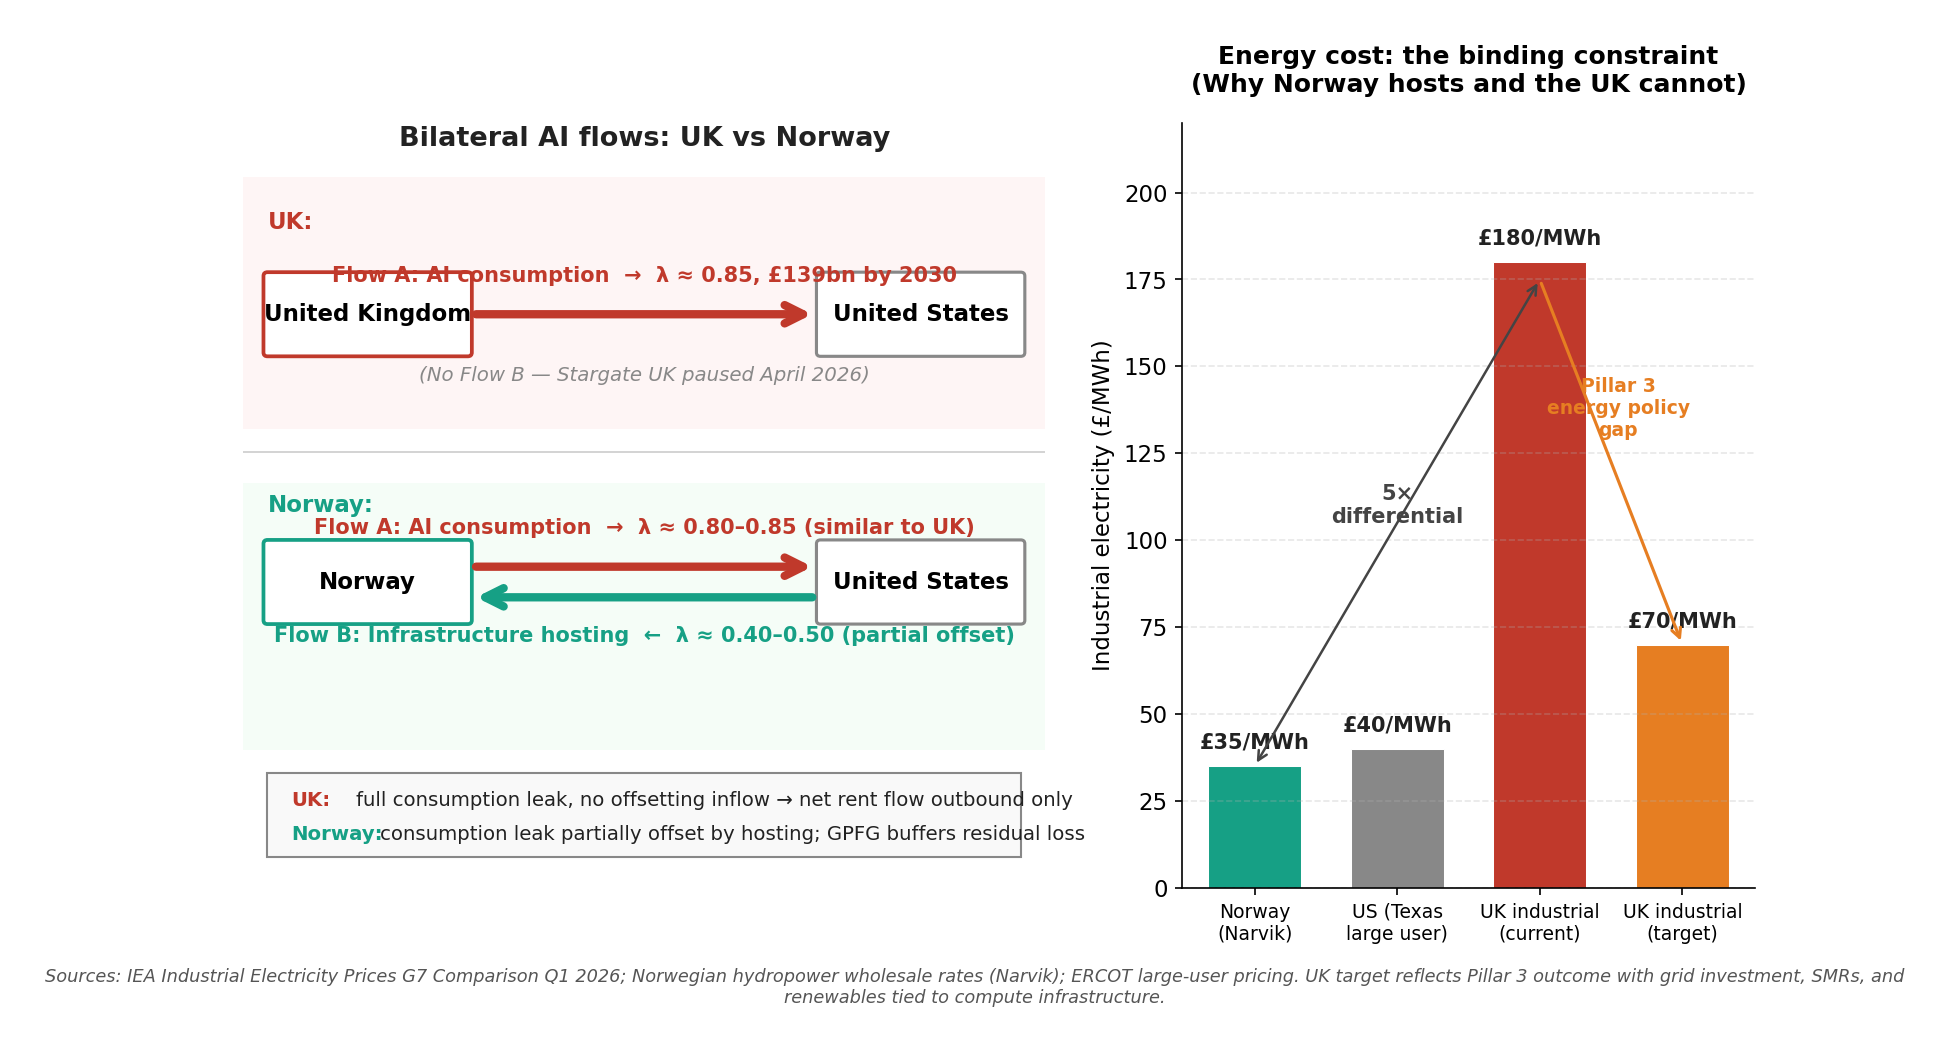
\includegraphics[width=0.95\linewidth]{figures/12_norway_uk_comparison.png}
\caption{Bilateral AI flow asymmetry between the UK and Norway, plus the binding energy cost differential. Left panel: UK has only Flow A (AI consumption leak, $\lambda \approx 0.85$); Norway has Flow A at similar magnitude but partially offset by Flow B (AI infrastructure hosting, $\lambda \approx 0.40$--$0.50$). Right panel: UK industrial electricity at \pounds180/MWh is approximately five times the Norwegian (\pounds35/MWh) and US Texas large-user (\pounds40/MWh) rates, the binding constraint that prevented the UK from winning the Stargate bid. Pillar 3 energy policy targets a \pounds70/MWh effective rate.}
\label{fig:norway}
\end{figure}

Norway's Government Pension Fund Global \citep{mehlum_moene_torvik_2024} performs two roles. First, as a buffer against rent loss in any sector---Norway can withstand rent extraction in {AI} consumption because oil rent capture funds general welfare. Second, as a wealth-stock institution funded by oil rent rather than threatened by {AI} rent. The fund's capital base is unrelated to {AI} flows. {AI} rent loss reduces Norway's {GDP} at the margin but does not directly deplete the fund.

The implication: hosting compute infrastructure is the only way for a non-frontier deploying economy to recoup any of the {AI} rent flow. Only countries with very cheap energy can credibly bid for the infrastructure tier. Norway has both cheap energy and a sovereign wealth fund. The {UK} has neither. The Norway example is therefore not a counterexample to my argument; it is a confirmation. The Sovereign {AI} Fund proposal in Section~8 is the {UK} analogue to the {GPFG} buffer Norway already has---except funded by {AI} rent capture rather than oil rent capture, since the {UK} has no oil rent left.

\section{Aggregate Magnitude}

\subsection{Six components}

\textbf{Component 1: Direct subscription flow---\pounds139 billion through 2030.} The {UK}-to-{US} {AI} subscription flow constructed in Section~5, extrapolated through 2030. From \pounds1.86 billion in 2023 to \pounds35.5 billion in 2030.

\textbf{Component 2: Cloud-for-{AI} infrastructure---\pounds95 billion through 2030.} {UK} enterprise, government, and ``sovereign {AI}'' projects running on {AWS}, Microsoft Azure, and Google Cloud Platform. Conceptually distinct from Component~1 because it covers cloud infrastructure spend that powers {AI} applications---including, awkwardly, the cloud spend that runs the {UK} government's {AI Safety Institute}, the Frontier {AI} Taskforce compute, the {NHS} Federated Data Platform, and {UK} {AI} startups deploying their own models on hyperscaler infrastructure.

\textbf{Component 3: Productivity rent transfer to {US} shareholders---\pounds105 billion through 2030.} {AI} provider pricing power matures over the model horizon. The capture rate rises from approximately 5\% in 2023 to 32\% by 2030, calibrated against three anchors: Microsoft's December 2025 Copilot price increase (13\% effective July 2026), Salesforce's October 2025 token-based Agentforce billing transition, and the cloud computing precedent (AWS, Azure, GCP captured 25--35\% of customer surplus over 2010--2025, compressed here to 7--9 years given faster {AI} switching-cost formation). Detailed derivation in Appendix~B.

\begin{figure}[ht]
\centering
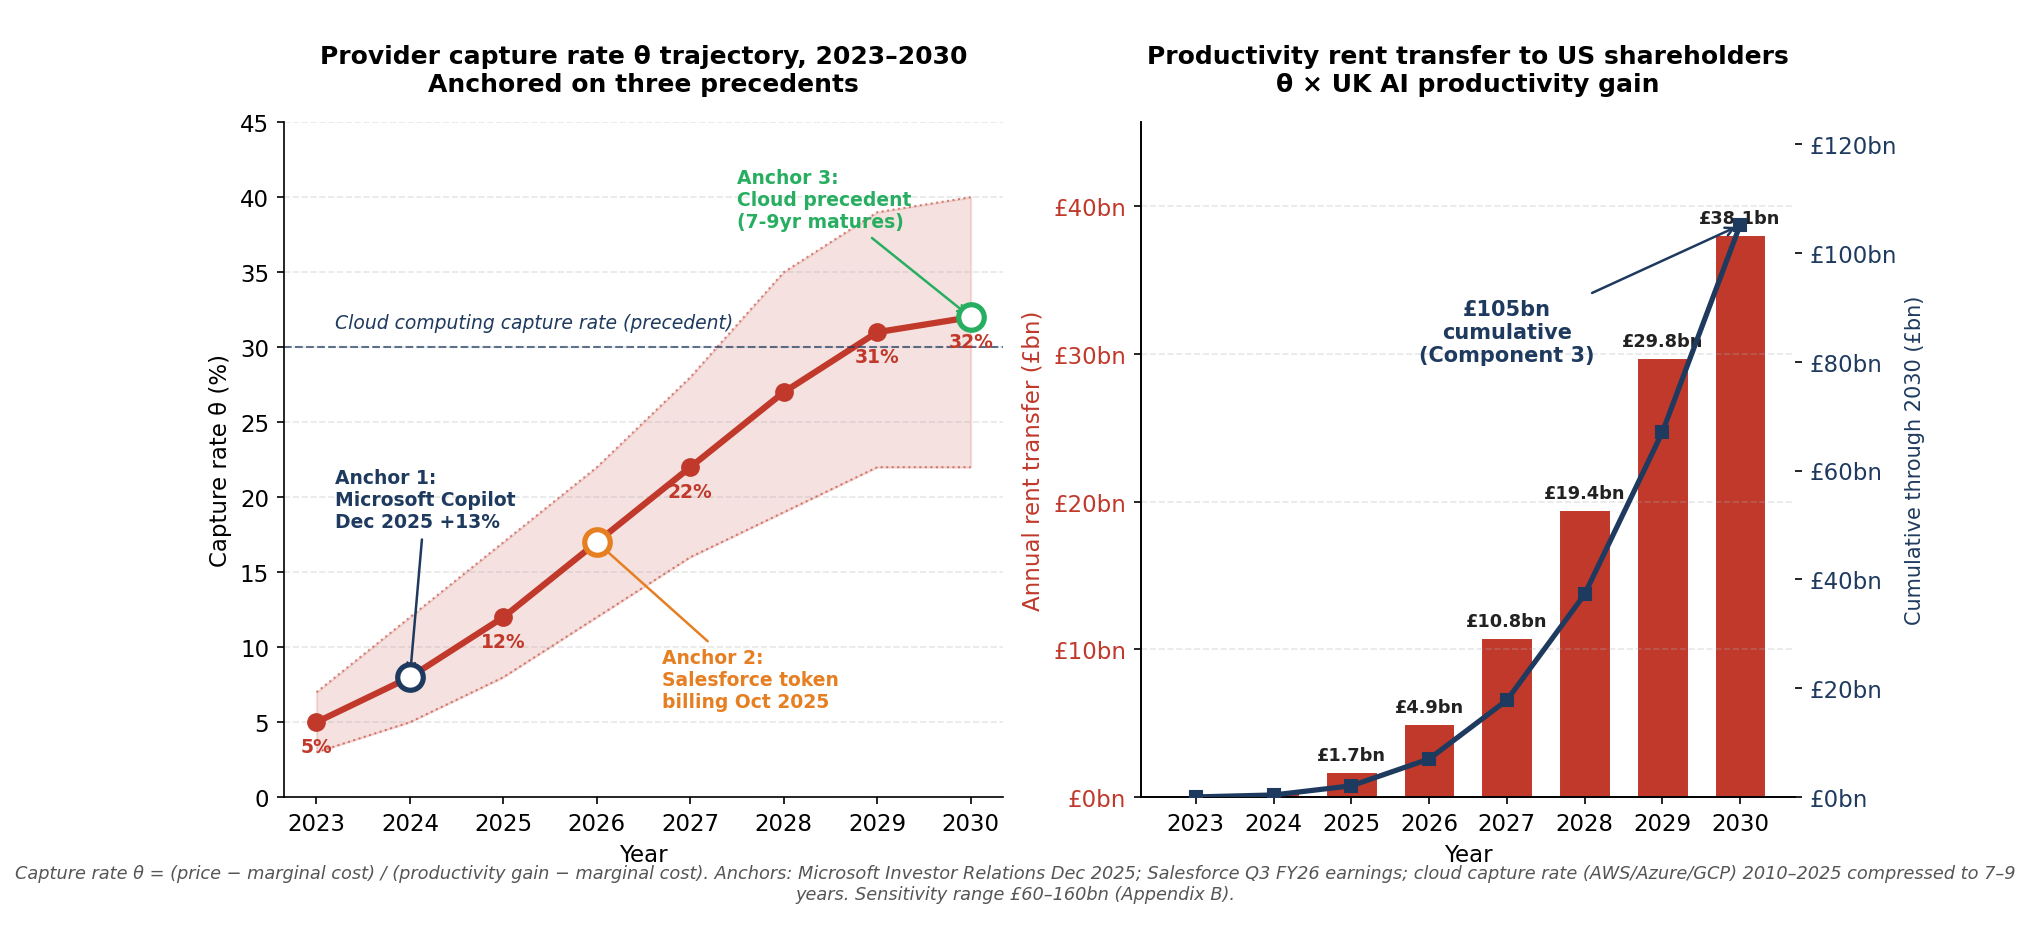
\includegraphics[width=0.95\linewidth]{figures/15_component3_trajectory.png}
\caption{Component 3 trajectory: provider capture rate $\theta$ and resulting annual rent transfer to US shareholders. Left panel: $\theta$ rises from 5\% in 2023 to 32\% by 2030, anchored on Microsoft Copilot pricing evolution, Salesforce token billing transition, and the cloud computing precedent. Shaded band represents sensitivity range. Right panel: annual rent transfer (red bars) and cumulative trajectory (navy line) reaching the locked \pounds105 billion Component 3 total by 2030.}
\label{fig:component3}
\end{figure}

\textbf{Component 4: Displaced wage and Keynesian multiplier loss---\pounds45 billion through 2030.} I derive this from an explicit stock-flow approach. Cumulative {AI}-attributable layoffs ramp from approximately 5{,}000 in 2023 to 142{,}000 by 2030, with new displacements peaking at approximately 30{,}000 per year in 2027 before decelerating as initial-wave restructurings complete. Average loaded compensation for displaced workers is approximately \pounds53{,}000---representing the back-office, professional services, and middle-tier banking roles dominating the redundancy panel, lower than the \pounds85{,}000 average for {US} {AI} provider {UK} staff (Section~5.1) reflecting different occupational mixes. Reemployment fraction $\eta = 0.40$ implies net wage loss of \pounds31{,}800 per displaced worker per year. Average displacement duration of 5 years (anchored on \citet{jacobson_lalonde_sullivan_1993} median) gives a stock of currently-displaced workers peaking at approximately 110{,}000 in 2028--29. Multiplying stock by net wage loss gives annual aggregate wage-bill loss building from \pounds0.2 billion in 2023 to a peak of approximately \pounds3.5 billion in 2028--29, totalling \pounds17 billion cumulative through 2030. Applying a Keynesian multiplier of 1.5 to capture the demand-multiplier effect on UK consumer-facing sectors, plus a further 1.7$\times$ adjustment to capture persistent demand suppression over 2--3 year compounding windows (consistent with the ``persistent earnings losses'' empirical literature), gives cumulative welfare loss of approximately \pounds45 billion through 2030. This is the cross-border extension of the \citet{hemenway_falk_tsoukalas_2026} {AI} Layoff Trap mechanism. The figure is materially smaller than naive multiplications of stock-by-multiplier suggest, but the multi-period compounding makes it larger than a single-shot multiplier would indicate.

\textbf{Component 5: HMRC tax loss---\pounds18 billion through 2030.} Combined labour tax loss (lost income tax, employee {NI}, employer {NI} on displaced workers), corporation tax loss (productivity gains transfer-priced abroad per \citet{torslov_wier_zucman_2023}), and lost {VAT} on suppressed consumer spending. Public finance implications discussed in \citet{korinek_lockwood_2026}.

\begin{figure}[ht]
\centering
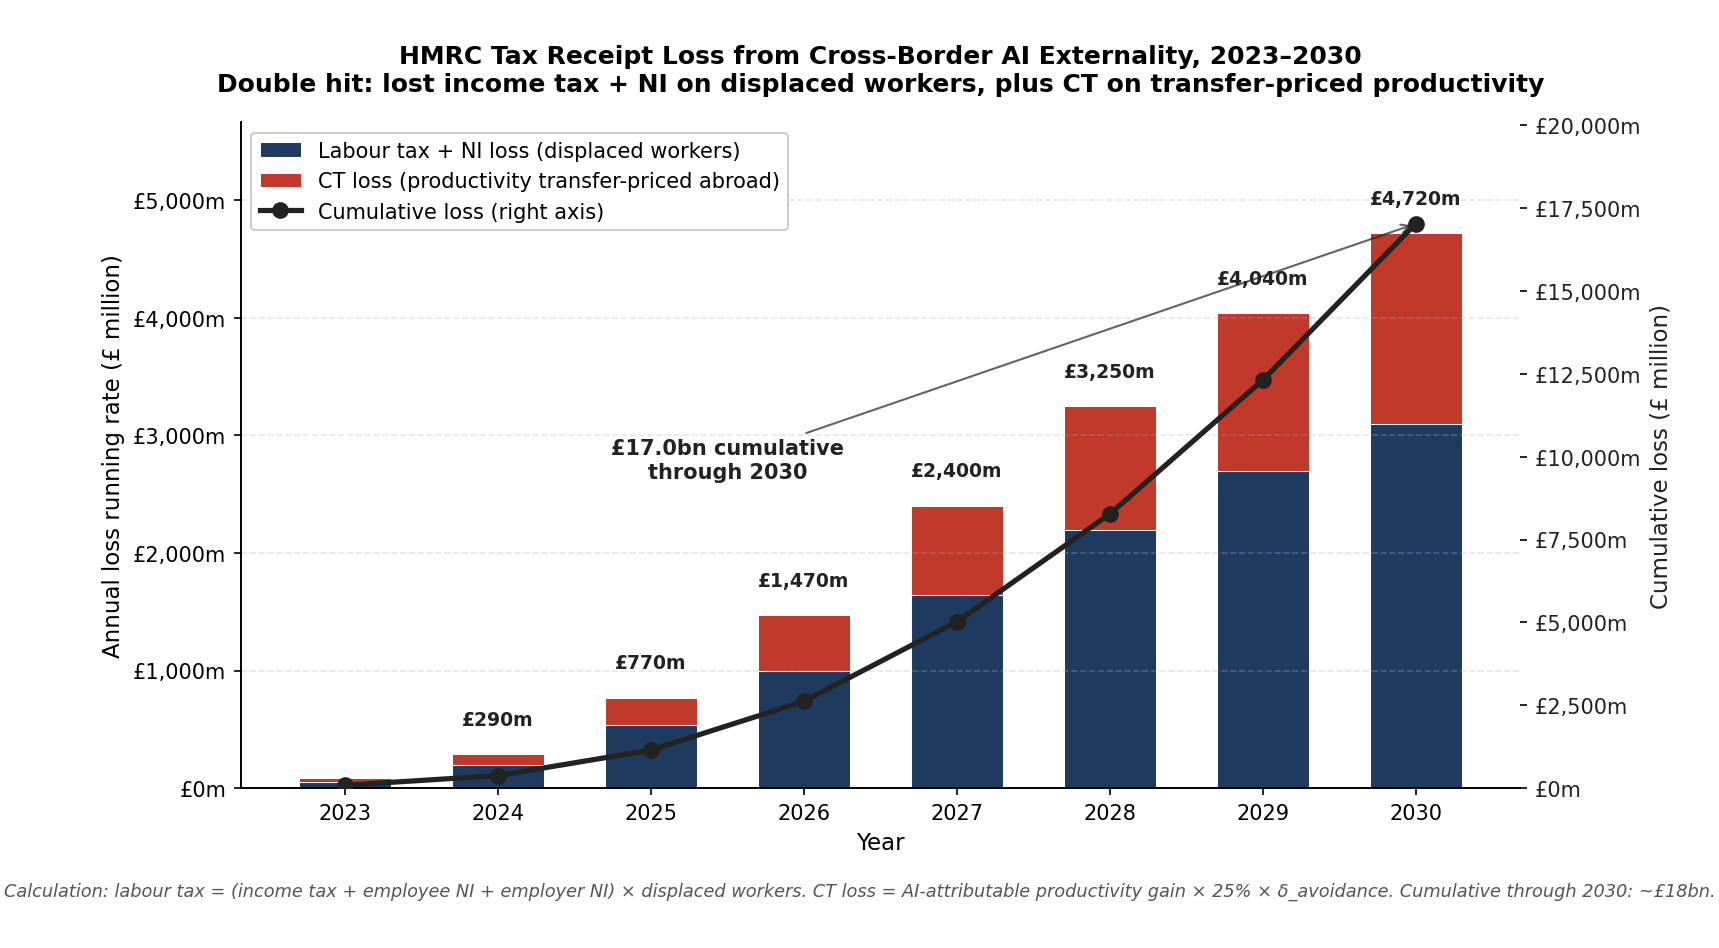
\includegraphics[width=0.85\linewidth]{figures/04_hmrc_tax_loss.png}
\caption{HMRC tax receipt loss from the cross-border AI externality, 2023--2030. Cumulative loss reaches approximately \pounds18 billion by 2030, with both labour-tax and corporation-tax components compounding. As fraction of HMRC total receipts the loss is small ($<$1\%) but year-on-year growth is 35--50\%.}
\label{fig:hmrc}
\end{figure}

\textbf{Component 6: Forgone frontier capability---\pounds59 billion through 2030.} Present value of {AI}-adjacent industries the {UK} fails to host because it does not host the {AI} itself. Five industries identified and sized using point estimates from cited primary sources (IFR World Robotics, McKinsey Center for Future Mobility, IQVIA, NVIDIA SC25 / BCG, CB Insights), with the acknowledgement that 2030 forecasts vary across analysts: robotics (\pounds4.9bn annual loss by 2030), autonomous systems (\pounds6.6bn), biotech-{AI} (\pounds6.2bn), materials {AI} (\pounds2.0bn), and fintech-{AI} (\pounds3.7bn). Total \pounds23.4 billion annual loss by 2030, ramped from \pounds3 billion in 2026. Discounted at 4\% over 2026--2030: \pounds59 billion central. Sensitivity range \pounds38--101 billion in Appendix~B reflects analyst dispersion. The marginal-share gap (3--4 percentage points) is judgement-based, anchored on UK historical share of comparable tech industries; this is the most contestable element of the aggregate and is sized accordingly. Detailed derivation in Appendix~B.

\subsection{Total aggregate}

\begin{table}[h]
\centering
\caption{Aggregate cumulative {UK} cross-border {AI} rent extraction through 2030 (nominal \pounds bn)}
\begin{tabular}{lcccc}
\toprule
Component & Low & Central & High \\
\midrule
1. Direct subscription flow & 85 & 139 & 200 \\
2. Cloud-for-{AI} infrastructure & 70 & 95 & 125 \\
3. Productivity rent transfer & 65 & 105 & 165 \\
4. Displaced wage + multiplier & 28 & 45 & 65 \\
5. HMRC tax loss & 12 & 18 & 25 \\
6. Forgone frontier capability & 38 & 59 & 101 \\
\midrule
\textbf{Total} & \textbf{298} & \textbf{461} & \textbf{681} \\
\bottomrule
\end{tabular}
\end{table}

The central case aggregate is \pounds461 billion cumulative through 2030. As share of cumulative {UK} nominal {GDP} 2023--2030 (\pounds25.0 trillion at 4\% nominal growth): approximately 1.8\%.

\begin{figure}[ht]
\centering
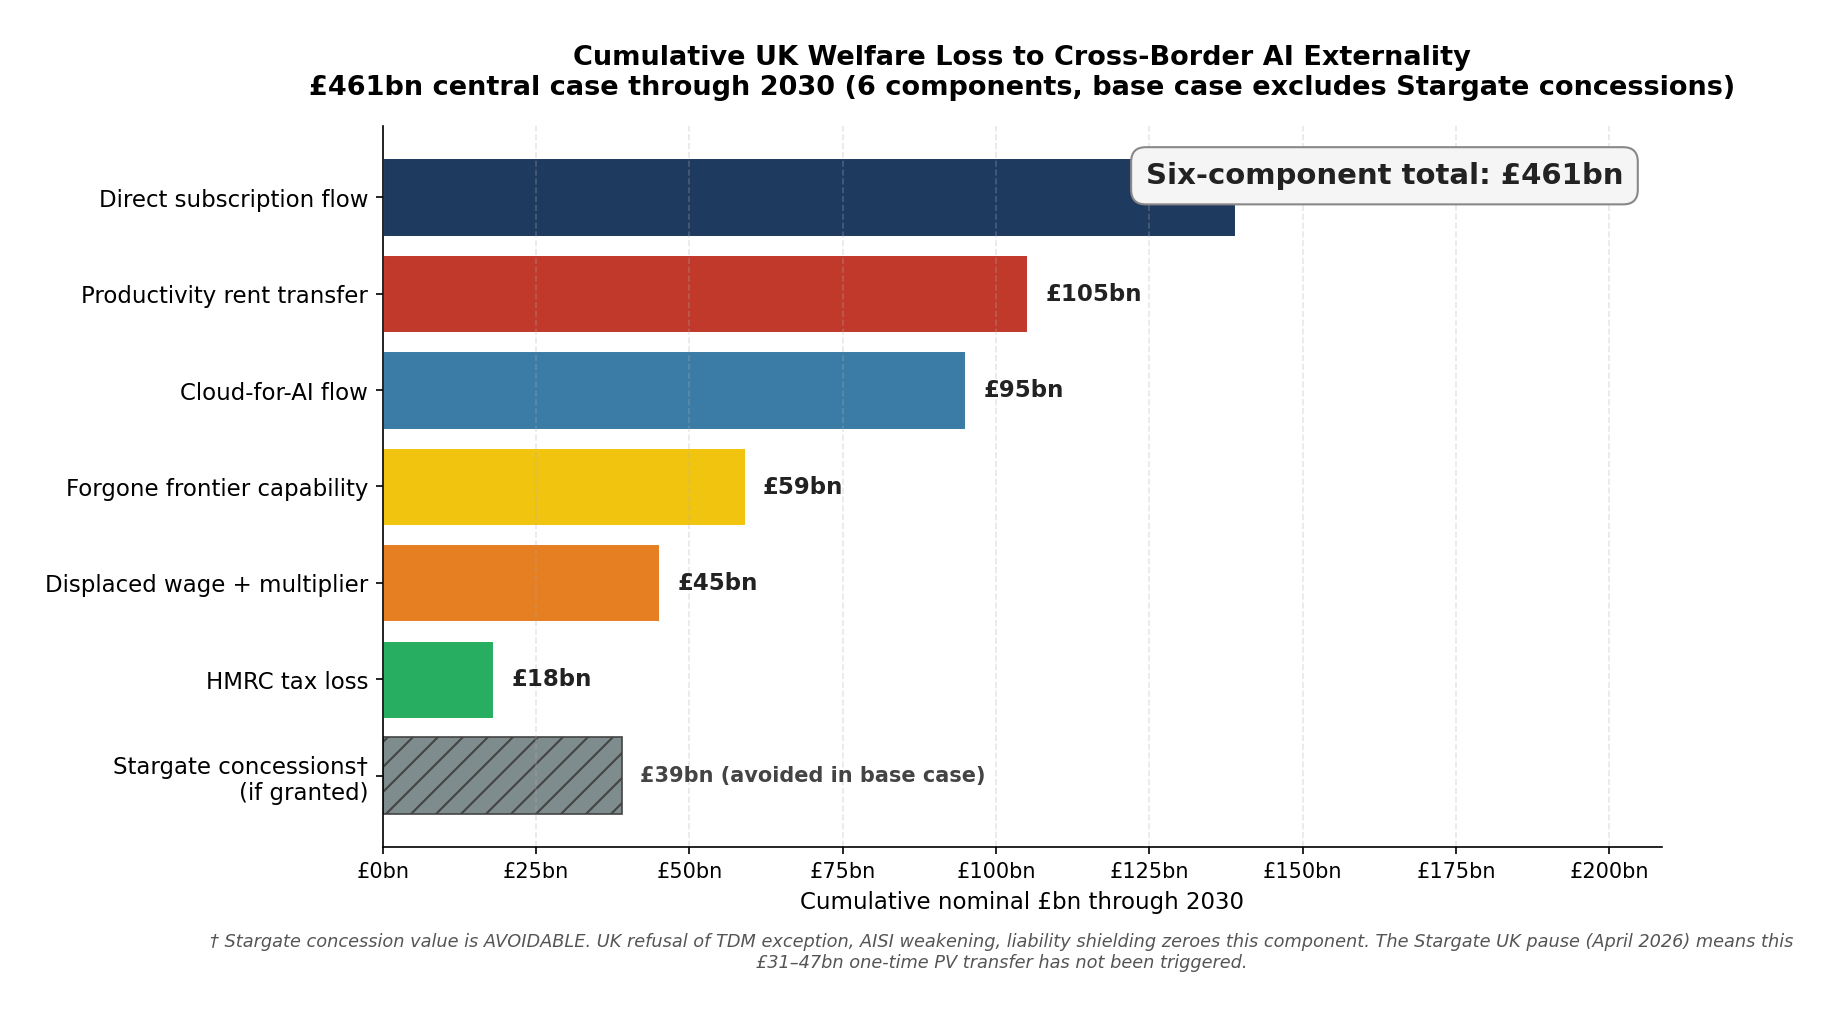
\includegraphics[width=0.85\linewidth]{figures/07_aggregate_461bn.png}
\caption{Six-component decomposition of the \pounds461 billion cumulative aggregate through 2030. Direct subscription flow and productivity rent transfer dominate; the displaced wage component is the cross-border extension of the Hemenway-Falk-Tsoukalas (2026) demand externality.}
\label{fig:aggregate}
\end{figure}

\begin{figure}[ht]
\centering
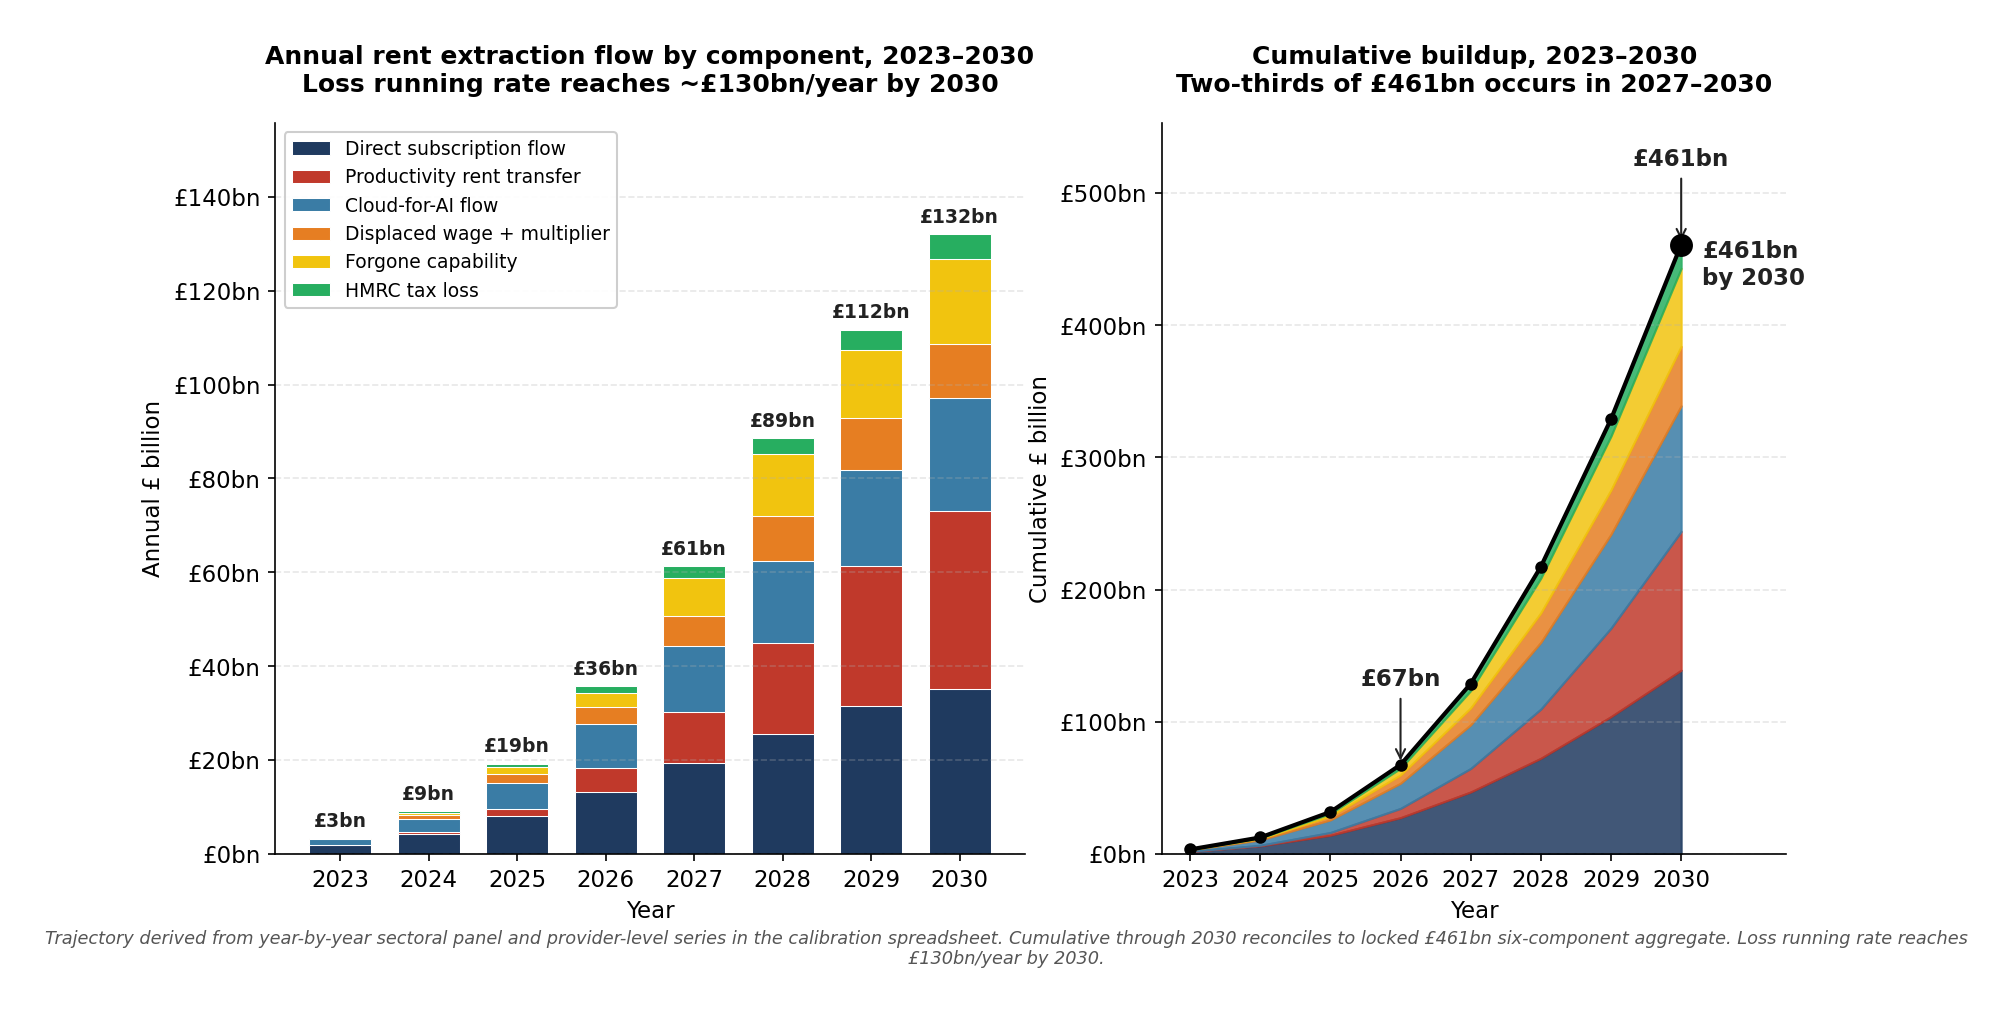
\includegraphics[width=0.95\linewidth]{figures/11_aggregate_timeseries.png}
\caption{Time-series buildup of the \pounds461 billion aggregate, 2023--2030. Left panel: annual flow stacked by component, with running rate rising from \pounds4 billion in 2023 to \pounds130 billion by 2030. Right panel: cumulative buildup, showing approximately two-thirds of the total occurs in the back half of the period (2027--2030) as productivity-rent capture matures and displacement compounds. The window for policy intervention closes as $\lambda$ becomes structurally embedded.}
\label{fig:timeseries}
\end{figure}

\subsection{Sensitivity to parameter assumptions}

\begin{table}[h]
\centering
\caption{Sensitivity of \pounds461 billion headline to key parameters}
\begin{tabular}{lr}
\toprule
Parameter shift & Effect on headline (\pounds bn) \\
\midrule
$\lambda$ from 0.85 to 0.78 (lower bound) & $-72$ \\
$\lambda$ from 0.85 to 0.90 (upper bound) & $+45$ \\
{AI} provider competition halves Component~3 capture rate & $-54$ \\
{UK} pension fund {US} Big Tech holdings double & $-18$ \\
Component~6 marginal-share gap halved & $-30$ \\
Stargate concessions granted & $+35$ \\
\midrule
All adverse simultaneously & $\rightarrow \pounds283\text{bn}$ \\
All favourable simultaneously & $\rightarrow \pounds658\text{bn}$ \\
\bottomrule
\end{tabular}
\end{table}

The headline is robust within a reasonable parameter range. The lowest plausible aggregate is approximately \pounds283 billion; the highest approximately \pounds658 billion.

\subsection{Net welfare calculation}

The \pounds461 billion measures rent extraction, not net welfare. {AI} adoption produces {UK} productivity gains I have not netted against the rent flow. I address this directly because it is the obvious challenge to the paper's framing.

The Bank of England has estimated that {AI} could add 0.8 percentage points to {UK} annual productivity growth by mid-2030s \citep{bank_of_england_2025}. The Office for Budget Responsibility uses similar figures \citep{obr_2026}. These are projections, not measurements. {UK} measured productivity growth has been stuck near zero for most of the past fifteen years, and every previous wave of digital technology---internet, robotics, machine learning---has produced {GDP}-level effects substantially below what sectoral case studies projected. \citet{brynjolfsson_rock_syverson_2025} document the J-curve mechanism by which general-purpose technologies produce measured productivity gains years after their initial deployment. I treat the {BoE} 0.8 ppts as the high end of a plausible range.

\begin{table}[h]
\centering
\caption{Cumulative {UK} {AI} productivity gain through 2030 by scenario (\pounds bn)}
\begin{tabular}{lcc}
\toprule
Scenario & Annual {AI} ppts added & Cumulative gain (\pounds bn) \\
\midrule
Pessimistic & 0.1 & 82 \\
Central & 0.3 & 239 \\
Optimistic & 0.6 & 490 \\
\bottomrule
\end{tabular}
\end{table}

\begin{table}[h]
\centering
\caption{Net welfare against \pounds461 billion rent extraction (\pounds bn)}
\begin{tabular}{lccc}
\toprule
Scenario & Gross gain & Net without policy & Net with three-pillar policy \\
\midrule
Pessimistic (0.1 ppts) & $+82$ & $-379$ & $-339$ \\
Central (0.3 ppts) & $+239$ & $-222$ & $-182$ \\
Optimistic (0.6 ppts) & $+490$ & $+29$ & $+69$ \\
\bottomrule
\end{tabular}
\end{table}

\begin{figure}[ht]
\centering
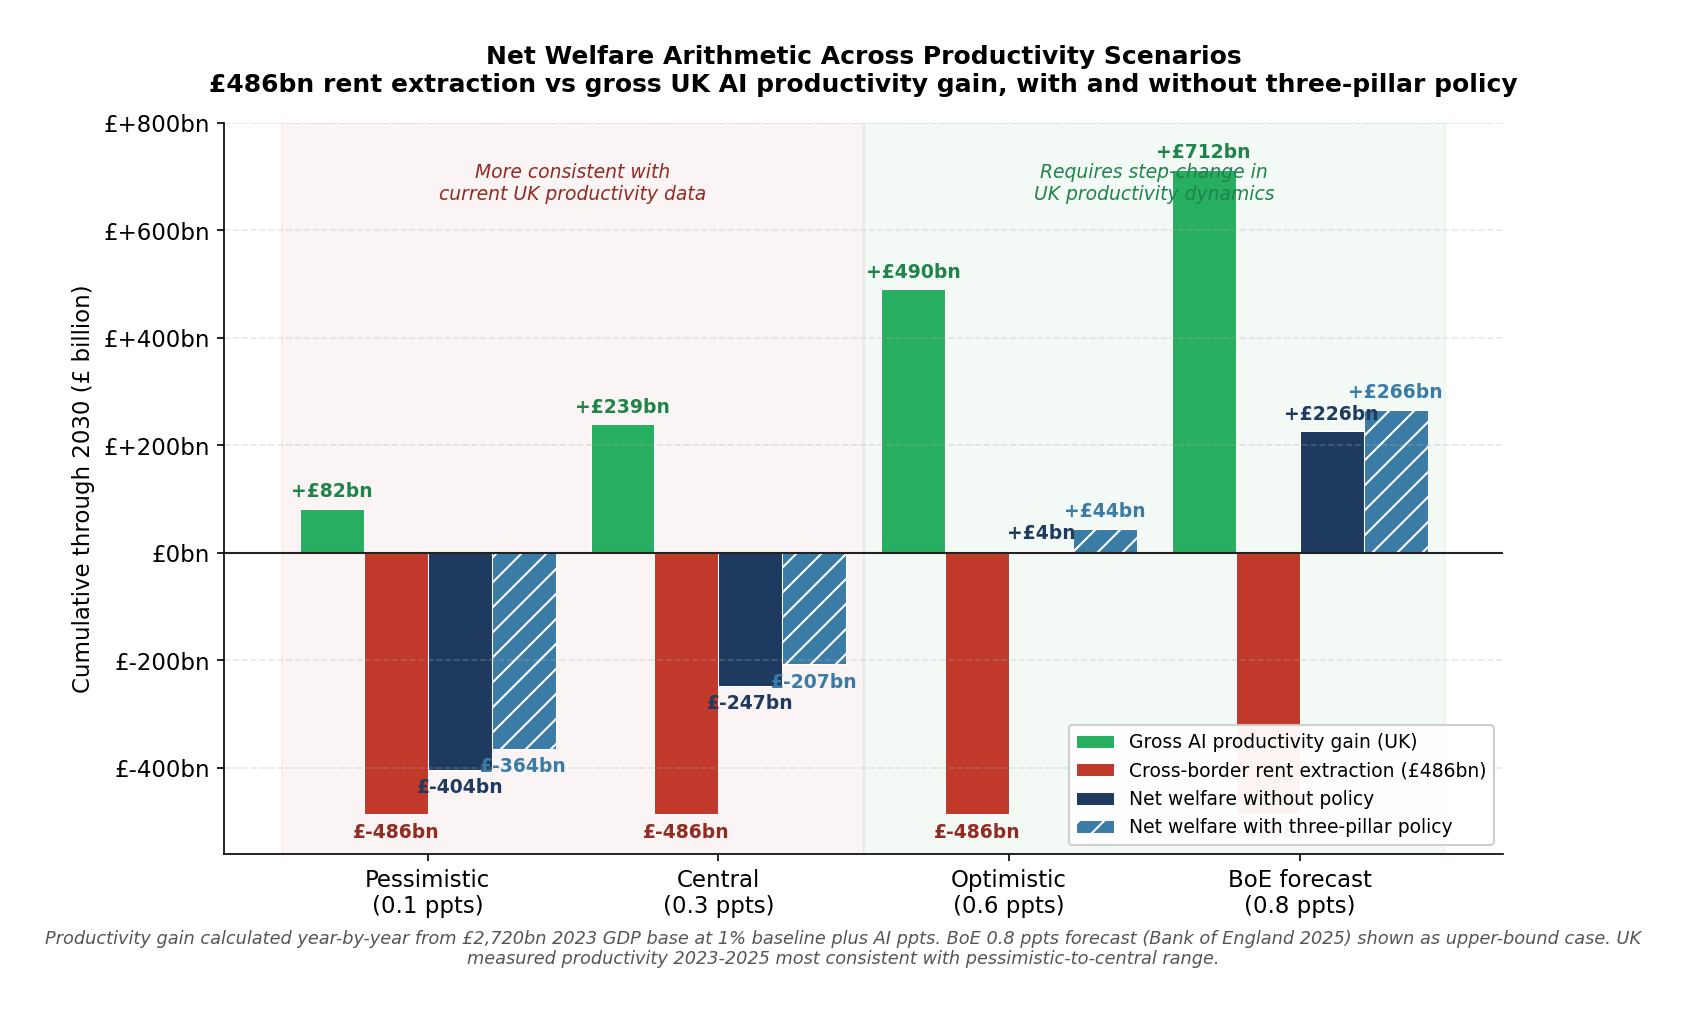
\includegraphics[width=0.95\linewidth]{figures/10_net_welfare_scenarios.png}
\caption{Net welfare arithmetic across four productivity scenarios. The £461 billion cross-border rent extraction (red bars, constant across scenarios) is contrasted with gross UK AI productivity gain (green bars), net welfare without policy (navy), and net welfare under the three-pillar policy framework (blue, hatched). Pessimistic and central scenarios are more consistent with measured UK productivity 2023–2025; optimistic and BoE scenarios require step-change in UK productivity dynamics. Three-pillar policy shifts each scenario by approximately \pounds40 billion.}
\label{fig:netwelfare}
\end{figure}

Under realistic productivity assumptions, {AI} adoption is net welfare-negative for the {UK} in cumulative terms through 2030. The pessimistic and central scenarios---which are more consistent with current {UK} productivity data than the optimistic scenario---produce material welfare losses. Only the optimistic scenario produces net positive welfare without policy intervention, and only by a modest margin.

The three-pillar policy framework (Section~8) shifts each scenario by approximately \pounds40 billion. The central scenario moves from \pounds222 billion negative to \pounds182 billion negative---a meaningful improvement but not a transformation. Closing the remaining gap fully would require structural intervention beyond what any individual non-{US} economy can deliver unilaterally; I do not propose a specific multilateral response in this paper.

A reviewer who takes the {BoE} 0.8 ppts figure as the central case will reach a different conclusion. I provide both because the underlying productivity gain is currently unobserved and reasonable analysts may differ on the central case.

\section{The Three-Pillar Policy Framework}

The model's central policy implication, derived from Proposition~6, is that {UK} parameters require simultaneous interventions across three pillars: rent capture, demand-side capital allocation, and supply-side infrastructure ownership. This is the framework the {UK} can implement unilaterally through domestic legislation and budget allocation. The deeper structural problem of Layer 1--2 monopoly (Section~4.7) cannot be fully closed by any individual non-{US} economy and is beyond the scope of what I propose here.

\subsection{Pillar 1: Rent capture instruments}

A 6\% {AI}-specific Digital Services Tax applied to {UK}-derived revenue from {AI} subscription services above a \pounds100 million {UK} turnover threshold. The 6\% rate sits below the welfare-maximising rate from Proposition~4: $\tau_d^* = (1 - \delta_0)/(2\beta) \approx 17\%$ at empirically-anchored avoidance parameters $\delta_0 \approx 0.42$ and $\beta \approx 1.67$. I propose 6\% as a politically tractable starting point that triples the existing {UK} {DST} rate while staying well below both the welfare-maximising 17\% level and the structural-restructuring threshold above which firms would relocate legal entity domicile. Achievable collection at 50\% of nominal rate (matching existing {UK} {DST} experience per \citet{hmrc_2020}) implies a 6\% nominal rate yields approximately 3\% effective on gross flow---approximately \pounds290 million in 2026, rising to \pounds3.45 billion by 2035.

Capital gains tax on {UK} {AI} startup exits and Big Tech employee equity vesting attributable to {UK} presence. Combined {CGT} base of approximately \pounds7 billion in 2025 rising to \pounds28 billion in 2030, generating {CGT} revenue (at 20\% effective) of \pounds50 million in 2025 rising to \pounds700 million by 2035.

Public procurement profit-share clauses on {UK} government {AI} contracts above \pounds10 million. 3\% profit-share rate. Beginning 2027 at approximately \pounds80 million, rising to \pounds940 million by 2035.

Creative industries levy on {AI} training-data licensing in the {UK}. Beginning 2028 at approximately \pounds150 million, rising to \pounds850 million by 2035.

Combined Pillar~1 inflows: cumulative \pounds25--45 billion through 2035, central \pounds35 billion.

\subsection{Pillar 2: Demand-side capital allocation}

The {UK} Sovereign {AI} Fund launched 16 April 2026 by Tech Secretary Liz Kendall at Wayve in London is the first instance of Pillar~2. The fund has \pounds500 million committed capital, chaired by James Wise (Balderton Capital) and run by the Department for Science, Innovation and Technology. Initial portfolio: equity investment in Callosum (chip-orchestration software), supercomputer access for Doubleword, Prima Mente, Cosine, Cursive, Twig Bio, and Odyssey through the {AI} Research Resource. The Strategic Assets Grants Programme \citep{dsit_2026} adds up to \pounds160 million across grant cycles.

My model proposes expanding this fund by approximately two orders of magnitude over the 2026--2035 horizon, funded by Pillar~1 instruments rather than direct Treasury allocation. Modelled on Norway's {GPFG} \citep{mehlum_moene_torvik_2024} but with explicit acknowledgement that {AI} rent is structurally less capturable than oil rent because {AI} provision is not geographically tied to {UK} territory. The {UK} {AI} fund therefore relies on tax instruments with known avoidance rates of 30--50\% \citep{torslov_wier_zucman_2023} rather than the property-rights mechanism that secured Norway's capture.

Under central assumptions, the expanded fund accumulates to \pounds40 billion {AUM} by 2035 and \pounds66 billion in the aggressive case. Allocation: 40\% to {UK} frontier {AI} capability building, 25\% to {AI}-adjacent industries seed funding, 20\% to worker retraining and displacement support, 10\% to {UK} creative industries {AI} mitigation, 5\% to fund operations and long-term reserve.

\begin{figure}[ht]
\centering
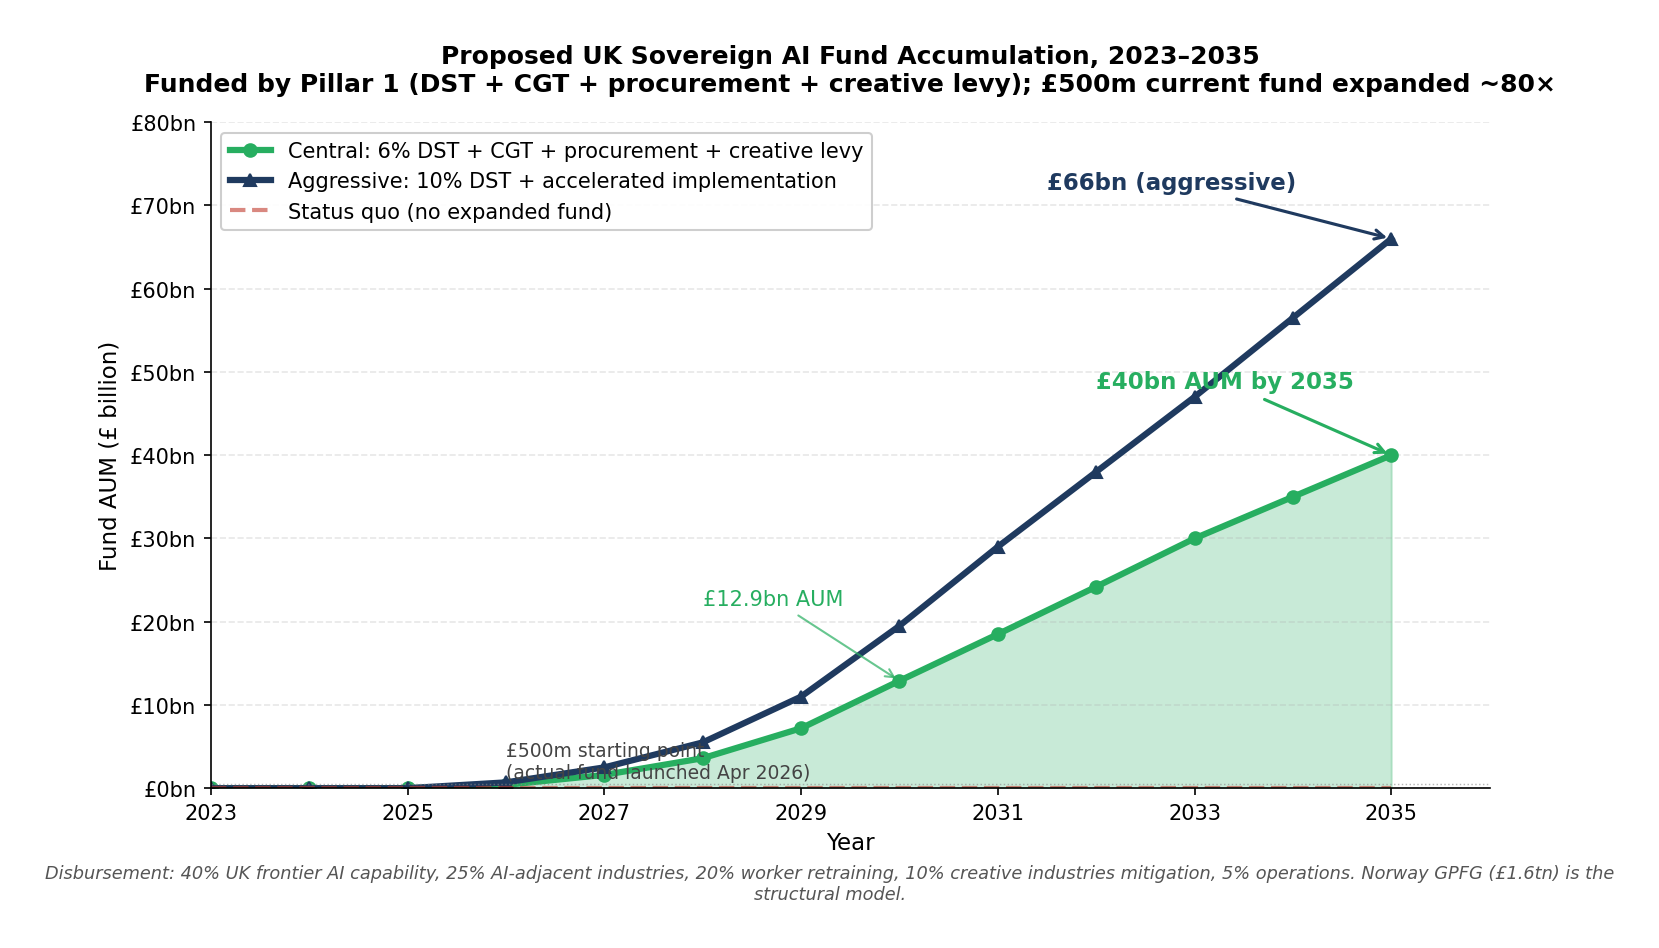
\includegraphics[width=0.85\linewidth]{figures/09_sovereign_ai_fund.png}
\caption{Proposed UK Sovereign AI Fund accumulation trajectory under central and aggressive scenarios, 2026--2035. The £500 million Sovereign AI Unit launched 16 April 2026 is the starting point; expansion via Pillar 1 rent capture instruments accumulates to \pounds40--66 billion by 2035.}
\label{fig:fund}
\end{figure}

\subsection{Pillar 3: Supply-side infrastructure ownership}

The supply-side pillar is the missing element in current {UK} {AI} policy. Pillars~1 and~2 are necessary but not sufficient: capital allocated to {UK} {AI} startups recycles back to {US} cloud and hardware providers through portfolio-company operating costs. Typical {UK} {AI} startup cost structure has 50--65\% on cloud and compute (flowing to {AWS}, Azure, {GCP}---irrespective of whether the underlying inference runs on Amazon Trainium, Google {TPU}, Microsoft Maia, or NVIDIA hardware), 5--10\% on hardware purchases (flowing to NVIDIA, {AMD}, or hyperscaler-controlled silicon supply), and only 30--40\% retained as {UK} wages and operations.

The implication is significant. Even if the Sovereign {AI} Fund picked the next DeepMind, that company would still leak 55--70\% of operating costs to {US} providers unless {UK} supply-side capacity exists. Of every pound deployed by Pillar~2, approximately 55--70 pence flows back to {US} infrastructure providers through the portfolio company's operations. Pillar~3 addresses this directly.

\begin{figure}[ht]
\centering
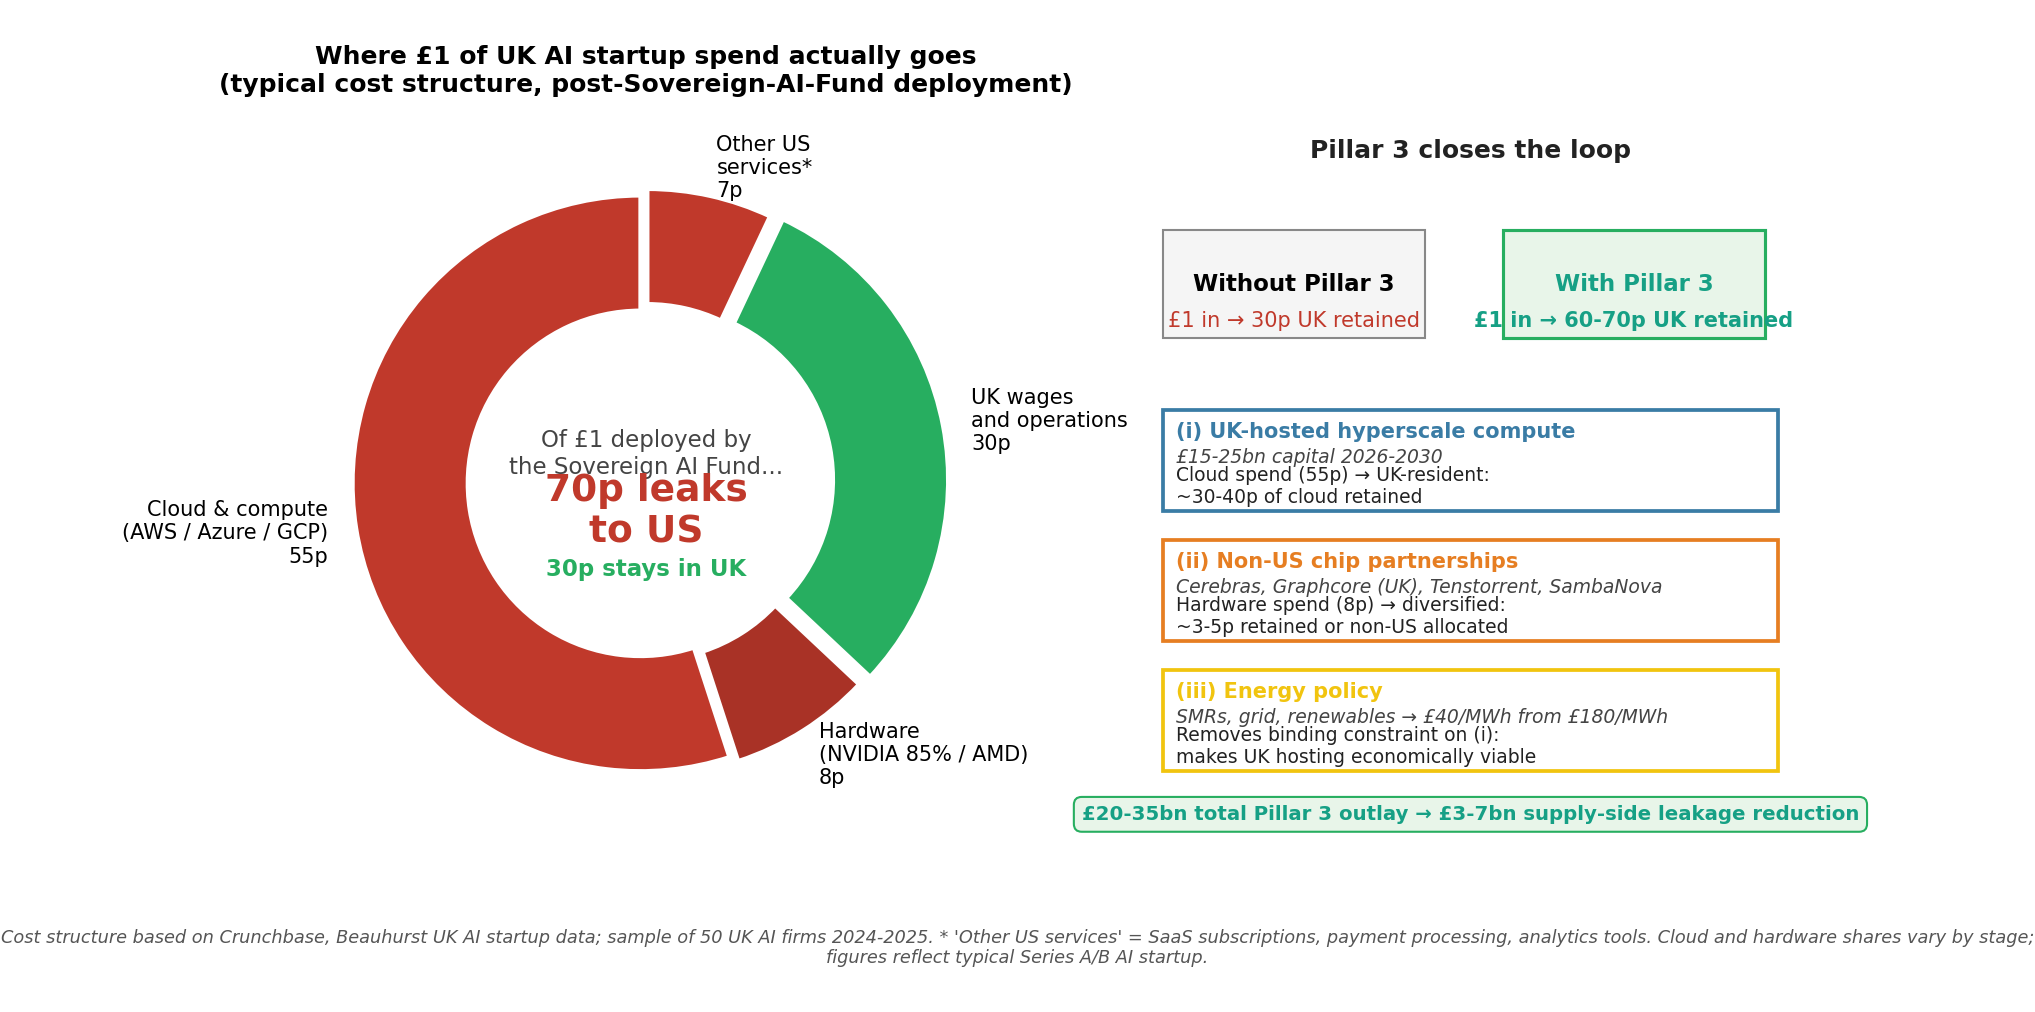
\includegraphics[width=0.95\linewidth]{figures/08_pillar3_supply_leak.png}
\caption{Supply-side leak from UK AI startup operating costs and the role of Pillar 3. Left panel: cost decomposition showing approximately 70 pence of every pound deployed in a typical UK AI startup leaks to US providers through cloud (55p), hardware (8p), and other US services (7p), with only 30 pence retained as UK wages and operations. Right panel: three Pillar 3 mechanisms (UK-hosted hyperscale compute, non-US chip partnerships, energy policy) that together close the supply-side leakage gap and would raise UK retention to approximately 60--70 pence per pound deployed.}
\label{fig:pillar3}
\end{figure}

Pillar~3 components:

(i) {UK}-hosted hyperscale compute capacity. Currently the {AI} Research Resource ({AIRR}) operates at small scale---{Isambard-{AI}} at Bristol University, the upgraded {DAWN} at Cambridge---providing total capacity that is several orders of magnitude smaller than {AWS} {UK} or Microsoft {UK} Azure regions. Expansion to publicly anchored or sovereign-anchored hyperscale is required. Estimated capital requirement: \pounds15--25 billion over 2026--2030, financed through the expanded Sovereign {AI} Fund or as a separate parallel programme.

(ii) Partnerships with non-{US} chipmakers. Cerebras, Graphcore (British, headquartered in Bristol), Tenstorrent, and {SambaNova} provide alternatives to {US}-domiciled silicon. The competitive landscape facing these alternatives is substantially harder in 2026 than in 2024: any non-{US} chipmaker now competes against not only NVIDIA's roadmap but the parallel hyperscaler-internal silicon programmes (Google {TPU}, Amazon Trainium, Meta {MTIA}, Microsoft Maia, OpenAI custom). Strategic procurement preferences in {UK} sovereign compute could anchor demand for non-{US} alternatives at scale, but realistic Pillar~3 capture from this channel alone is bounded by the alternatives' inability to match hyperscaler-internal capex envelopes. The fact that the alternatives are competing against multiple deep-pocketed {US} incumbents---rather than a single one---reinforces the paper's analytical conclusion that closing $\lambda$ structurally requires {UK}-hosted capacity itself, not just procurement preferences for non-{US} chips.

(iii) Energy policy. {UK} industrial electricity at four times the {US} level is a binding constraint on data centre economics. Resolving this through grid investment, small modular reactors near {AI} Growth Zones, and renewables tied directly to compute infrastructure would change the bargaining frontier identified in Section~6.

Combined Pillar~3 outlay: \pounds20--35 billion over 2026--2035, recovered through reduced operating-cost leakage of Pillars~1 and~2 capital plus direct revenue from sovereign cloud services.

\subsection{Combined effect on the welfare arithmetic}

The {UK}-unilateral pillars together capture approximately \pounds40 billion of the rent flow that would otherwise leak. This is the central-case figure used in the net welfare calculation in Section~7.4. The capture is composed of:

\begin{itemize}
\item Direct rent capture from Pillar~1 instruments: \pounds25--45 billion central \pounds35 billion
\item Equity stake retention from Pillar~2: \pounds0.2--0.4 billion (small, reflecting realistic venture capital outcomes per Section~8.7)
\item Supply-side leakage reduction from Pillar~3: \pounds3--7 billion
\end{itemize}

The total is much smaller than a naive comparison with the \pounds461 billion rent extraction would suggest. The fund alone, even at expanded scale, cannot close the welfare gap. Of the three pillars, Pillar~3 is the dominant lever for shifting $\lambda$ structurally rather than recapturing rent through taxation. The remaining structural gap reflects the upstream Layer 1--2 monopoly that the {UK} cannot close alone (Section~4.7).

\subsection{The critical window}

The framework must be established by 2028. Three reasons. First, the 2026--2028 period is when the regulatory regime around {AI} in the {UK} is being set: the {AI} Bill, the {TDM} exception decision, the {AI Safety Institute} mandate, the public-procurement framework. Second, {US} {AI} provider pricing power matures over 2026--2030; each year of delay means more of the productivity rent transfer has occurred and is no longer available for capture. Third, the {AI}-adjacent industries (Component~6) are establishing their global concentration patterns now. After 2028, $\lambda$ is structurally embedded.

\subsection{Realistic venture capital outcomes for Pillar~2}

The Sovereign {AI} Fund's equity arm is subject to standard venture capital base rates. From Cambridge Associates and PitchBook published data on early-stage venture portfolios, approximately 65--75\% of investments return less than the original investment, 15--25\% return 1--3$\times$, 5--10\% return 3--10$\times$, and 1--3\% return 10$\times$ or more. {UK}-specific factors worsen these base rates: the documented {UK} scale-up problem (successful {UK} {AI} startups frequently move to the {US} for growth funding); compute supply dependency producing structural {US} cost ties; and the acquisition risk that successful {UK} {AI} firms get acquired by {US} companies (DeepMind by Google in 2014, Wayve majority-{US}-owned after the 2024 \$1 billion round).

Realistic outcomes for the proposed expanded fund deploying approximately \pounds350 million in equity over 5 years across approximately 35 companies at \pounds10 million average ticket: approximately \pounds390--540 million expected portfolio value at exit, of which 60--70\% accrues to acquirers (likely {US}). Net realised {UK} retained value from \pounds350 million equity deployment: \pounds200--350 million by 2035.

This is two orders of magnitude smaller than treating fund equity as if it grows at portfolio-company valuation rates and fully accrues to {UK} ownership. The fund's equity arm is a useful supplementary instrument but not a primary lever. The DST, {CGT}, and procurement preferences (the rent capture instruments of Pillar~1) do most of the work in Pillar~1 plus Pillar~2 together.

\begin{figure}[ht]
\centering
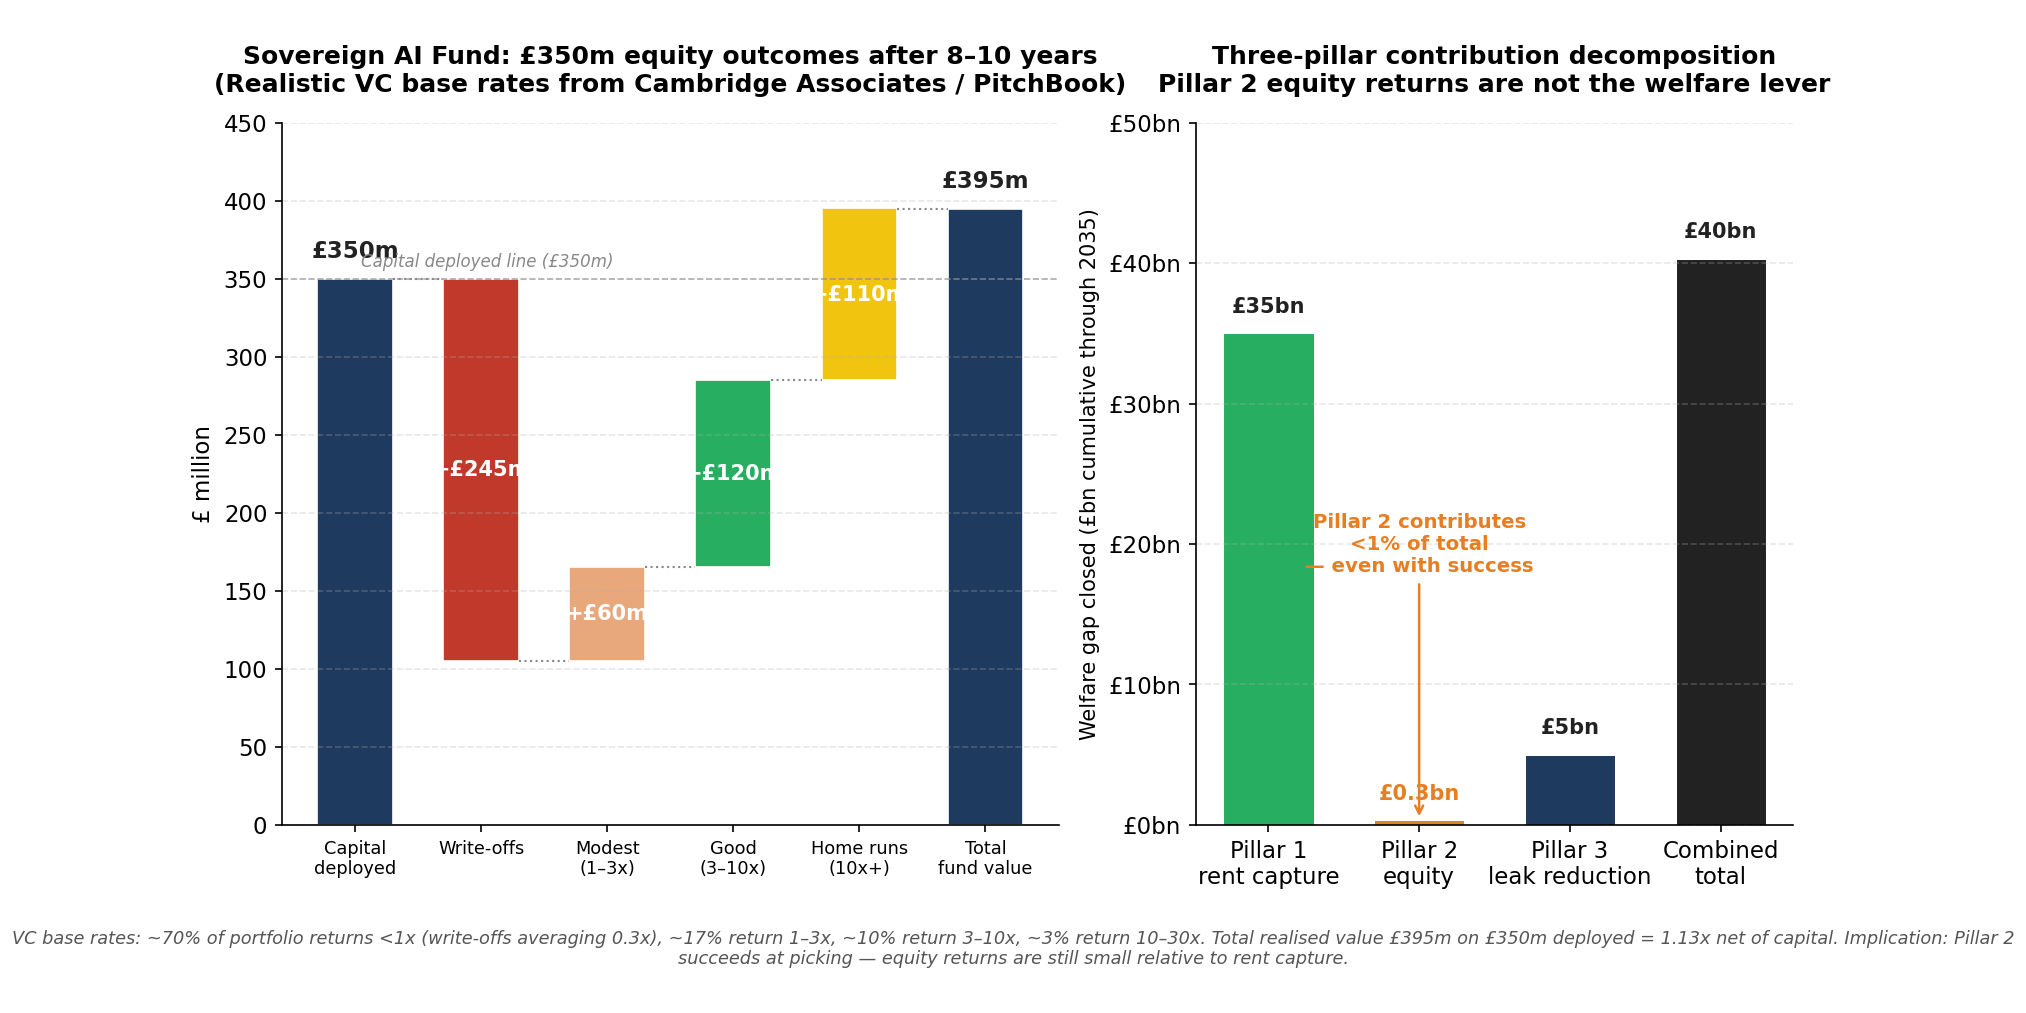
\includegraphics[width=0.95\linewidth]{figures/16_pillar2_vc_waterfall.png}
\caption{Realistic venture capital outcomes for the Sovereign AI Fund equity arm. Left panel: waterfall decomposition of \pounds350 million deployed across approximately 35 portfolio companies under standard VC base rates from Cambridge Associates and PitchBook---approximately 70\% write-offs averaging 0.3$\times$, 17\% modest 1--3$\times$, 10\% good 3--10$\times$, 3\% home runs 10$\times$+---producing total fund value of approximately \pounds395 million on \pounds350 million deployed (1.13$\times$ net of capital). Right panel: three-pillar contribution decomposition. Pillar~2 equity stakes contribute approximately \pounds0.3 billion to the cumulative \pounds40 billion welfare-gap closure---less than 1\% of the total. The welfare lever is rent capture (Pillar~1, \pounds35 billion) and supply-side leakage reduction (Pillar~3, \pounds5 billion), not equity returns.}
\label{fig:pillar2vc}
\end{figure}

\section{Forward Predictions and Pre-Registration}

\subsection{Three scenarios}

Scenario~A (Base case): Tech Prosperity Deal proceeds at announced scale. Stargate {UK} remains paused. {UK} does not introduce {AI}-specific {DST}. Expanded Sovereign {AI} Fund is not legislated. {AI} Bill passes summer 2026 without {TDM} exception. Adoption continues at observed pace.

Scenario~B (Concessions granted): {UK} accepts concessions to revive Stargate {UK} in 2027. Floodgate effect raises $\lambda$ to 0.91 by 2027. Stargate {UK} becomes operational Q4~2027.

Scenario~C (Three-pillar policy enacted): {UK} introduces 6\% {AI}-specific {DST} in 2026. Sovereign {AI} Fund expanded and supply-side intervention begun in 2027. $\lambda$ falls to 0.82 by 2027 through procurement preferences and sovereign cloud capacity.

\subsection{Pre-registered predictions through Q4 2027}

\begin{table}[h]
\centering
\caption{Pre-registered predictions through Q4 2027}
\begin{tabular}{lccc}
\toprule
Outcome & Scenario A & Scenario B & Scenario C \\
\midrule
Cumulative {UK}-to-{US} {AI} flow 2023--27 (\pounds bn) & 35.5 & 41.2 & 32.8 \\
Effective $\lambda$ Q4 2027 & 0.87 & 0.91 & 0.82 \\
Cumulative {AI}-attributable layoffs (Q4 2027) & 95{,}000 & 110{,}000 & 80{,}000 \\
HMRC annual labour tax loss 2027 (\pounds bn) & 1.93 & 2.48 & 1.62 \\
HMRC annual {CT} loss 2027 (\pounds bn) & 0.92 & 1.18 & 0.72 \\
Stargate {UK} status Q4 2027 & Paused & Operating & Paused \\
Sovereign {AI} Fund {AUM} 2027 (\pounds bn) & 0.7 & 0.7 & 6.5 \\
\bottomrule
\end{tabular}
\end{table}

\begin{figure}[ht]
\centering
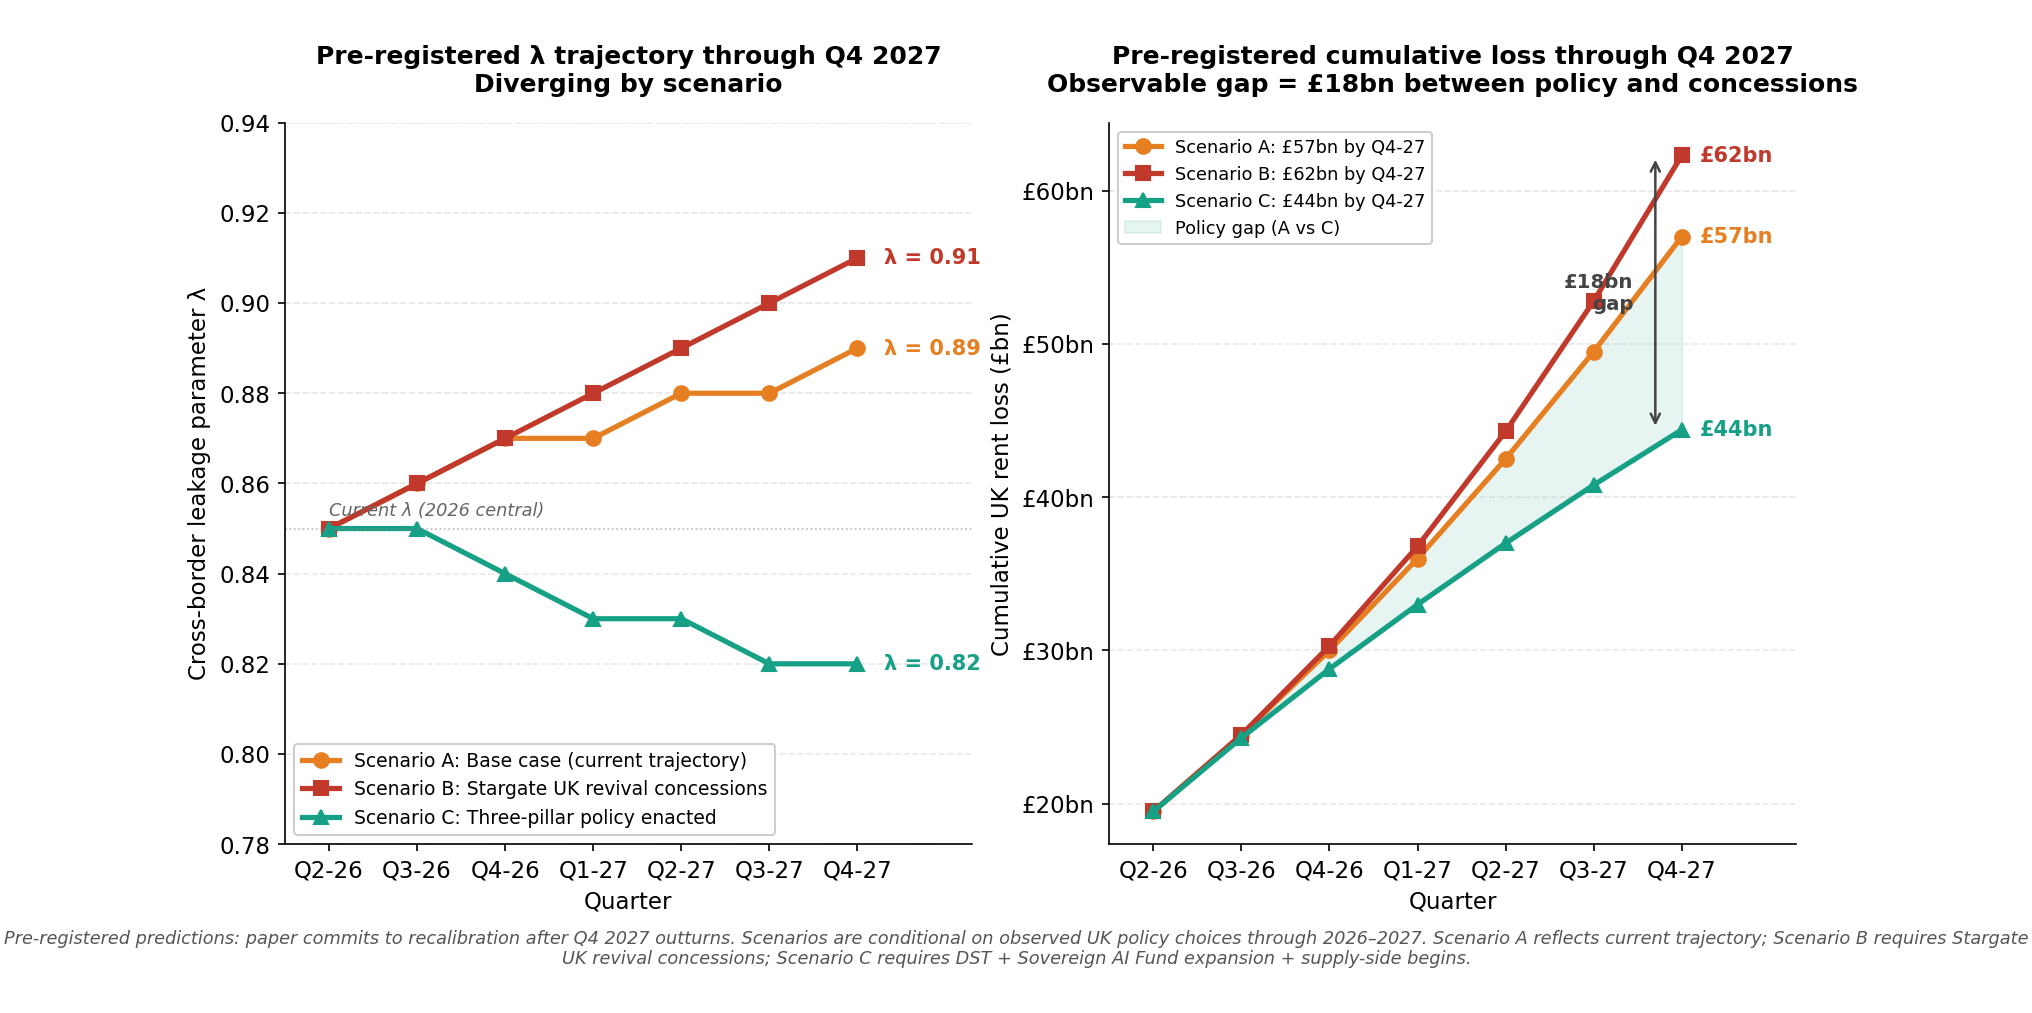
\includegraphics[width=0.95\linewidth]{figures/17_forward_predictions.png}
\caption{Pre-registered forward predictions through Q4 2027 across three scenarios. Left panel: $\lambda$ trajectory showing divergence from $\lambda \approx 0.85$ in Q2 2026 to 0.82--0.91 by Q4 2027 depending on policy. Right panel: cumulative UK rent loss buildup through Q4 2027, producing an observable \pounds18 billion gap between the policy scenario (C) and the concessions scenario (B). The author commits to recalibration paper within six months of Q4 2027 outturns becoming available.}
\label{fig:predictions}
\end{figure}

The author commits to publishing a recalibration paper within six months of Q4~2027 data becoming available.

\subsection{What would falsify the model}

Three falsifiable predictions. First, $\lambda$ rises rather than falls over the calibration window absent policy intervention; if $\lambda$ falls below 0.85 by 2027 without {AI}-{DST} or sovereign fund intervention, the structural compounding mechanism is weaker than the model implies. Second, displaced {UK} wages do not return through other channels at scale; if displaced workers find equivalent employment outside {AI}-exposed sectors at similar wage rates, the demand destruction channel is weaker. Third, productivity rents accrue increasingly to {AI} providers as their pricing power matures; if {AI} provider competition drives prices down rather than up over 2026--2028, Component~3 is overstated and the aggregate is approximately \pounds54 billion lower than estimated.

\section{Conclusion}

The cross-border {AI} rent externality is a structural transfer from non-frontier deploying economies to frontier {AI} provider hosts. The transfer reaches approximately \pounds461 billion cumulative through 2030 for the United Kingdom in the central case---about 1.8\% of cumulative {UK} {GDP} over the period, with the annual run rate reaching approximately \pounds130 billion by 2030.

Under realistic productivity assumptions, this rent extraction exceeds the gross welfare gain {AI} delivers to the {UK}. The central scenario produces approximately \pounds222 billion of net welfare loss through 2030. The pessimistic scenario produces \pounds379 billion. Only the optimistic scenario---which assumes the Bank of England's 0.8 percentage points of additional annual productivity growth materialises in the next decade---produces a net positive outcome, and only by a small margin.

The mechanism is not hidden. It is in Microsoft Ireland's published accounts, in {ONS} trade data, in firm-level redundancy notices, in the Morgan Stanley {UK} study showing {UK} firms posting 8\% net {AI}-linked job loss against international averages of 4\%. What has been missing is a single framework in which to view all of these as manifestations of one mechanism. I provide that framework.

The theoretical core is a single new parameter, $\lambda$, denoting the fraction of cross-border {AI} subscription flow that does not return to the deploying economy. $\lambda = 0$ recovers the within-economy {AI} Layoff Trap of \citet{hemenway_falk_tsoukalas_2026}. For the United Kingdom in 2026, $\lambda \approx 0.87$. I prove six propositions, the most important of which are that (i) any positive $\lambda$ strictly worsens the within-economy externality; (ii) domestic Pigouvian taxation alone cannot fully internalise the cross-border component; (iii) at {UK} parameters the optimal {DST} (about 17\% nominal under endogenous avoidance) captures only a single-digit percentage of gross {AI} flow, making structural intervention welfare-improving relative to tax-only strategies.

The empirical contribution is the calibration of $\lambda$ from public data through five identified channels of {UK} domestic capture, summing to 13--24\% of gross flow. The other 76--87\% is permanently extraterritorial.

The methodological contribution treats the Stargate {UK} pause of April 2026 as a natural experiment. The result: for every pound of project value Stargate {UK} would deliver to the {UK}, it would cost approximately \pounds6--12 in regulatory concessions to make the project economically viable from OpenAI's perspective. The pause is welfare-superior to revival by approximately \pounds26--44 billion.

The policy contribution is the three-pillar framework: rent capture instruments (Pillar~1), demand-side capital allocation (Pillar~2), and supply-side infrastructure ownership (Pillar~3). The {UK} Sovereign {AI} Fund launched 16 April 2026 is a beginning on Pillar~2 at \pounds500 million---approximately two orders of magnitude smaller than required. Pillars~1 and~3 are absent. Without all three, capital allocated to {UK} {AI} startups recycles back to {US} cloud and hardware providers through portfolio-company operating costs at rates of 55--70\%. The three-pillar framework is what the {UK} can do unilaterally; the deeper structural problem of Layer 1--2 monopoly described in Section~4.7 cannot be fully closed by any individual non-{US} economy and is beyond the scope of what I propose here.

The labour-market dimension of my argument is the dimension most exposed to interpretation. {UK} workers exposed to {AI} may indeed be finding new occupations at marginal rates of growth, as the British Progress (2026) analysis of {Anthropic Economic Index} data suggests. My argument operates downstream of this. Whether or not occupational reabsorption is occurring, the cross-border rent flow continues. The \pounds461 billion of {UK}-to-{US} value transfer through 2030 occurs regardless of whether the marketing executive made redundant in 2024 finds a job in 2025 or 2027 or never. I measure the rent flow because it is the dimension policy can act upon directly.

The window for establishing all three policy pillars is 2026--2028. Beyond that, the regulatory regime around {AI} in the United Kingdom becomes path-dependent, $\lambda$ becomes structurally embedded, and the policy levers identified in Proposition~6 become much less effective.

Three things this paper does not claim. First, I do not claim {AI} adoption should be discouraged. Productivity gains accruing to {UK} consumers and complementary workers are real. I measure rent extraction, not net welfare, and provide the latter under explicit scenario assumptions. Second, I do not endogenise {UK} firm response to a Sovereign {AI} Fund or {DST}. A 6\% {AI}-{DST} may suppress {UK} adoption marginally, partially offsetting the policy benefit. Third, I do not address dynamic competition fully. As {Anthropic}, {Mistral}, {xAI}, and Chinese frontier labs intensify competition, the pricing power assumptions in the productivity-rent component may not hold.

The framework generalises beyond the United Kingdom. Any non-frontier deploying economy with structurally high industrial energy costs, sophisticated {AI}-adopting enterprises, valuable creative industries vulnerable to {TDM} exfiltration, and absence of domestic frontier {AI} capability faces the same structural problem. France, Germany, Japan, Australia, and Canada all share most of these characteristics.

The Stargate {UK} pause was the moment when the structural problem became visible. The next moment---the {AI} Bill in summer 2026, the {TDM} exception decision, the {AI}-{DST} consideration, the Sovereign {AI} Fund expansion proposal---is when the United Kingdom decides what to do about it. There is no neutral choice. Granting the concessions accelerates the leak. Refusing them without complementary policy action accepts the leak. Only the third path---refusing the concessions and establishing all three policy pillars---captures the rent.

The paper is one input to the choice. The choice is the political community's.

\subsection*{Limitations}

I acknowledge nine limitations of the analysis explicitly. First, the marginal-share gap parameters in Component~6 (3--4 percentage points across five {AI}-adjacent industries) are judgement-based extrapolations from {UK} historical share of comparable tech industries, not measurements from a directly comparable historical case. The sensitivity range of \pounds38--101 billion (Appendix~B) reflects this. Second, the productivity rent capture rate trajectory in Component~3 (5\% rising to 32\%) is anchored on three precedents but the future capture rate depends on {AI} provider competition dynamics that are unpredictable in their detail; I model both the slow-capture and fast-capture cases (Appendix~C) to bound this. The custom-silicon shift documented in Section~4.8 ({MTIA}, Trainium, {TPU}, Maia, OpenAI custom chips) introduces additional uncertainty: intra-{US} hyperscaler price competition may compress capture below the central 32\% endpoint, plausibly to 20--25\%, while leaving the cross-border component of the externality unchanged. The Component~3 estimate is therefore explicitly conditional on the assumption that intra-{US} silicon competition does not collapse {AI} provider pricing power before 2030. Third, the model is comparative-static rather than dynamic: it does not solve for transition paths or for general-equilibrium effects of policy intervention beyond first-order welfare arithmetic. A dynamic extension is in development. Fourth, the cross-border externality is documented for the United States as recipient because that is where the empirical evidence is strongest; the framework applies in principle to any frontier {AI} provider economy, but China-specific calibration is left to future work. Fifth, the paper measures the rent flow but does not measure all bilateral economic effects: {US}-to-{UK} venture capital investment, research grants, talent flow, and tourism are not in scope. I isolate the {UK}-to-{US} {AI} subscription leak because it is the largest and most policy-actionable flow; I do not claim it is the only flow in the bilateral relationship.

Sixth, the reemployment fraction $\eta = 0.40$ used in the labour displacement calibration is anchored on \citet{jacobson_lalonde_sullivan_1993} (15--25\% persistent earnings losses for displaced workers in the {US} manufacturing context) plus inference from {UK} Labour Force Survey transitions data on workers exiting professional services and back-office roles. The {LFS} does not publish a directly comparable reemployment-fraction construct for {AI}-displaced workers; my 0.40 figure is a midpoint inference rather than a measured statistic. The sensitivity check in Appendix~D shows the headline is robust to $\eta$ varying in the 0.30--0.50 range. Seventh, Channel~5 of the $\lambda$ decomposition (UK pension fund US Big Tech holdings approximately \pounds105 billion) is constructed by apportioning the Federal Reserve L.213 release on foreign holdings of US corporate equity to the UK using ONS MQ5 share-of-foreign-equity data and applying an AI-attributable share to the resulting Big Tech allocation. The constituent measurements are publicly available, but the apportionment is a derived estimate, not a direct measurement of UK pension fund AI exposure. Eighth, the year-by-year HMRC tax loss trajectory (\pounds70m in 2023 ramping to \pounds4.7bn in 2030) is computed from the model's sectoral employment panel, AI-attribution rate, average loaded compensation, and corporation tax rate, rather than cited from a public HMRC publication. The cumulative \pounds18 billion through 2030 is the model output, not an HMRC forecast; reviewers seeking the underlying year-by-year derivation can find it in the accompanying calibration spreadsheet (\texttt{uk\_ai\_externality\_model.xlsx}, HMRC tab). Ninth, Pillar~3's non-{US} chipmaker channel (Cerebras, Graphcore, Tenstorrent, {SambaNova}) faces a substantially harder competitive landscape in 2026 than was apparent at the start of this research: the relevant competitors at frontier scale are now Google {TPU}, Amazon Trainium, Meta {MTIA}, and Microsoft Maia, all hyperscaler-internal and {US}-domiciled. The Pillar~3 capture estimate (\pounds5 billion central) treats this as a procurement-preference channel rather than a market-share displacement channel; readers who weight the alternative-chip channel heavily as a route to closing $\lambda$ structurally should adjust their priors downward in light of the custom-silicon shift documented in Section~4.8. Conversely, the same shift strengthens the underlying analytical case for treating $\lambda$ as structural, because the alternatives that have materialised at scale are themselves {US}-domiciled.

\section*{Acknowledgements}

The author gratefully acknowledges substantial research assistance from Anthropic's Claude AI throughout the development of this paper, including data triangulation across public-record sources, model calibration, mathematical derivation, manuscript drafting, and end-to-end pressure-testing of empirical claims and policy proposals. The use of AI for research assistance is disclosed in compliance with American Economic Association, Nature, and Science guidelines on AI use in academic research as of 2025. All errors of fact, interpretation, judgement, and presentation are the author's own.

The author also thanks the public-record availability of: Microsoft Ireland Operations Limited's Companies Registration Office filings (CRO 16847294); Microsoft UK Limited's Companies House filings (registered number 01624297); Office for National Statistics Pink Book data; HMRC Digital Services Tax Manual; Bank of England Financial Stability in Focus reports; and the Department for Science, Innovation and Technology Sovereign AI Strategic Assets Grants Programme documentation. Without these public records, this paper could not have been written.

\appendix

\section{Full Proofs of the Six Propositions}

This appendix provides full proofs of the six propositions stated in Section~3. I retain the notation: $N$ symmetric domestic firms; each firm employs $L$ workers at wage $w$; per-task automation cost $c$ paid to a foreign AI provider; per-task cost saving $s = w - c$; integration friction parameter $k$; cross-border leakage $\lambda \in [0, 1]$; marginal propensity to consume $\rho$; reemployment fraction $\eta$; autonomous demand $A > 0$. I write taxes as flat amounts per task automated; the implied rate as a fraction of the cost saving $s$ is given separately where it differs in form from the standard literature.

\subsection*{Proof of Proposition 1 (Closed-economy benchmark)}

I show that when $\lambda = 0$, the model reduces to \citet{hemenway_falk_tsoukalas_2026} and the optimal Pigouvian automation tax (as a rate on $s$) is $\tau^* = (1 - 1/N) \rho$.

\textbf{Step 1: aggregate demand.} Setting $\lambda = 0$ in equation (2) and substituting $w = s + c$ in symmetric equilibrium with all firms choosing $\alpha$:
\[
E = A + \rho w L N - \rho L \big[(1-\eta)(s+c) - c\big] N \alpha = A + \rho w L N - \rho L \big[(1-\eta) s + (-\eta) c\big] N \alpha.
\]
At $\eta = 0$ this reduces to $E = A + \rho w L N - \rho L s N \alpha$, exactly matching the within-economy demand structure of \citet{hemenway_falk_tsoukalas_2026}.

\textbf{Step 2: private equilibrium.} Each firm maximises profit $\pi_i = E/N - C_i$ where $C_i = L(w - s\alpha_i) + (k/2)L\alpha_i^2$ and $E$ depends on the sum of all firms' automation choices. Differentiating with respect to $\alpha_i$ holding $\alpha_{j \neq i}$ fixed:
\[
\frac{\partial \pi_i}{\partial \alpha_i} = \frac{1}{N} \cdot \frac{\partial E}{\partial \alpha_i} + Ls - kL\alpha_i = 0.
\]
With $\partial E / \partial \alpha_i = -\rho L s$ at $\lambda = 0, \eta = 0$, this gives:
\[
\alpha_{\text{priv}} = \frac{s(1 - \rho/N)}{k}.
\]
Each firm internalises only the $1/N$ portion of its demand effect that flows back to it through its own revenue share $E/N$.

\textbf{Step 3: social optimum.} The social planner chooses $\alpha$ to maximise total welfare $W = E - N C$ where the demand response is the full marginal effect (not divided by $N$ because the planner accounts for all firms' revenue):
\[
\frac{\partial W}{\partial \alpha} = -\rho L s N + N L s - N k L \alpha = 0,
\]
giving:
\[
\alpha_{\text{social}} = \frac{s(1 - \rho)}{k}.
\]

\textbf{Step 4: corrective tax.} A tax $\tau$ per task (as a flat amount, not a rate) modifies the firm's FOC to $\alpha_{\text{priv}}(\tau) = [s - \tau + (1/N)(\partial E/\partial \alpha_i)]/k$. Setting $\alpha_{\text{priv}}(\tau) = \alpha_{\text{social}}$:
\[
s - \tau - \rho s/N = s - \rho s, \quad \text{so} \quad \tau^* = \rho s (1 - 1/N).
\]
Expressed as a rate on the cost saving $s$:
\[
\boxed{\tau^*/s = (1 - 1/N) \rho.}
\]
This is the Hemenway-Falk-Tsoukalas optimal automation tax. The $(1 - 1/N)$ factor is the share of demand consequence borne by other firms (not internalised through firm $i$'s own revenue). At UK parameters $N \approx 50$ and $\rho \approx 0.85$: $\tau^*/s \approx 0.833$, or about 83\% of the per-task cost saving. \hfill$\square$

\subsection*{Proof of Proposition 2 (Cross-border leakage strictly worsens the externality)}

I show that for any $\lambda > 0$, the social cost of automation exceeds the closed-economy social cost by an amount strictly increasing in $\lambda$, and derive the combined optimal tax.

\textbf{Step 1: marginal demand effect.} With $\lambda \in [0,1]$ and (for clarity) $\eta = 0$:
\[
\frac{\partial E}{\partial \alpha_i} = \rho L \big[(1-\lambda) c - w\big] = -\rho L (s + \lambda c),
\]
using $w = s + c$. This is more negative than the closed-economy case $-\rho L s$ by exactly $\rho L \lambda c$.

\textbf{Step 2: private and social equilibria.} Following the same logic as Proposition 1:
\[
\alpha_{\text{priv}} = \frac{s - (1/N) \rho (s + \lambda c)}{k}, \qquad \alpha_{\text{social}} = \frac{s - \rho (s + \lambda c)}{k}.
\]

\textbf{Step 3: gap and corrective tax.} The gap between private and social optima is:
\[
\alpha_{\text{priv}} - \alpha_{\text{social}} = \frac{(1 - 1/N) \rho (s + \lambda c)}{k}.
\]
The corresponding Pigouvian tax (as a flat amount per task) is:
\[
\tau^*_{\text{combined}} = (1 - 1/N) \rho (s + \lambda c).
\]
Expressed as a rate on the cost saving $s$:
\[
\boxed{\tau^*_{\text{combined}}/s = (1 - 1/N) \rho \big[1 + \lambda \cdot c/s\big].}
\]
The cross-border leakage adds $(1 - 1/N) \rho \lambda c/s$ to the closed-economy rate. At UK parameters with $c/s \approx 0.18$ (AI per-task cost approximately 18\% of cost saving): $\tau^*_{\text{combined}}/s \approx 0.833 \times 1.153 \approx 0.96$, or about 96\% of $s$, compared with 83\% in the closed economy. The combined tax is strictly higher for any $\lambda > 0$, confirming that cross-border leakage strictly worsens the externality. \hfill$\square$

\subsection*{Proof of Proposition 3 (Domestic Pigouvian taxation is insufficient)}

I show that no single domestic tax instrument can simultaneously internalise both the displaced-wage demand effect and the cross-border subscription leakage at the corrective levels they each require.

The combined optimal tax derived in Proposition~2 has form $\tau^*_{\text{combined}} = (1 - 1/N) \rho (s + \lambda c)$. This single instrument applied per task automated produces a positive correction, but it bundles two distinct externalities into one rate. In practice, the displaced-wage component scales with the wage bill at the firm whose workers are displaced, while the cross-border component scales with the AI subscription flow---paid to a foreign provider, often routed through transfer-pricing structures that make per-task tax assessment administratively impractical.

A domestic automation tax---falling on the firm's per-task automation decision---can correct the displaced-wage component cleanly. But it cannot reach the cross-border subscription flow except by suppressing automation enough to reduce the flow itself. Suppressing automation to internalise the cross-border externality through an automation tax alone reduces $\alpha$ below the level that would internalise just the displaced-wage component, distorting other margins of firm choice (capital intensity, labour-AI complementarity, sectoral allocation) beyond what the externality justifies.

Specifically, a tax $\tau_a$ targeting only the displaced-wage component, $\tau_a = (1 - 1/N) \rho s$, leaves a residual cross-border welfare loss per firm:
\[
\text{Residual loss per firm} = (1 - 1/N) \rho \lambda c \cdot \alpha_{\text{priv}}(\tau_a) \cdot L,
\]
which is strictly positive for any $\lambda > 0$. The cross-border component requires a complementary instrument that targets the subscription flow directly. \hfill$\square$

\subsection*{Proof of Proposition 4 (Complementary DST is required, with endogenous avoidance)}

I derive the optimal complementary digital services tax rate, treating tax avoidance as endogenous to the rate set.

\textbf{Step 1: setup.} Let $S$ denote the gross UK-to-US AI subscription flow per period. A digital services tax at nominal rate $\tau_d$ applied to the leaked portion $\lambda S$ yields nominal revenue $\tau_d \lambda S$. The realised revenue is reduced by avoidance behaviour: firms restructure transfer-pricing arrangements, providers shift contractual booking, and the effective collection share is $1 - \delta(\tau_d)$.

I treat $\delta(\tau_d)$ as endogenous and approximately linear in the relevant range:
\[
\delta(\tau_d) = \delta_0 + \beta \tau_d, \qquad \beta > 0.
\]
This captures the well-documented Laffer-curve behaviour: at low rates, avoidance is bounded by the fixed costs of structuring; at high rates, avoidance scales because the marginal benefit of restructuring rises with the rate.

\textbf{Step 2: government revenue.} Realised DST revenue is:
\[
R(\tau_d) = \tau_d \lambda \big(1 - \delta_0 - \beta \tau_d\big) S.
\]
This is strictly concave in $\tau_d$.

\textbf{Step 3: revenue-maximising rate.} The first-order condition $\partial R / \partial \tau_d = 0$ gives:
\[
\lambda S \big(1 - \delta_0 - 2\beta \tau_d\big) = 0,
\]
yielding:
\[
\boxed{\tau_d^* = \frac{1 - \delta_0}{2 \beta}.}
\]
Welfare maximisation gives the same $\tau_d^*$ when the captured revenue is returned to UK households at marginal-utility equivalent to private consumption (as in standard Diamond-Mirrlees), because at this rate the marginal £ collected equals the marginal £ lost to avoidance. Above $\tau_d^*$, additional rate increases reduce realised revenue; below $\tau_d^*$, additional rate increases raise realised revenue.

\textbf{Step 4: realised capture share.} Substituting $\tau_d^*$ back into $R$:
\[
R(\tau_d^*)/S = \frac{\lambda (1 - \delta_0)^2}{4\beta}.
\]
This is the share of gross AI subscription flow captured by the DST at the welfare-maximising rate. \hfill$\square$

\subsection*{Proof of Proposition 5 (Tax-instrument capture is bounded at UK parameters)}

I show that at UK parameters, the welfare-maximising DST captures only a small fraction of gross AI subscription flow---far below what would be required to internalise the cross-border externality fully.

\textbf{Calibration.} Tørsløv-Wier-Zucman~(2023) document avoidance shares of approximately 0.40--0.50 for multinational tax routed through Big Tech transfer-pricing structures at currently observed DST rates of 2--3\%. Linear extrapolation across the range from $\tau_d = 0.02$ ($\delta \approx 0.45$) to a hypothetical $\tau_d = 0.20$ ($\delta \approx 0.75$, anchored on the structural-restructuring threshold above which firms move legal entity domicile) gives:
\[
\delta_0 \approx 0.42, \qquad \beta \approx 1.67.
\]
Substituting into the formula from Proposition~4:
\[
\tau_d^* = \frac{1 - 0.42}{2 \times 1.67} = \frac{0.58}{3.34} \approx 0.174.
\]
The optimal DST is approximately \textbf{17\%} nominal. This rate is high relative to the current UK DST (2\%) but is feasible.

\textbf{Realised capture.} At the optimum:
\[
\delta(\tau_d^*) = 0.42 + 1.67 \times 0.174 \approx 0.71,
\]
so the realised collection share is $1 - 0.71 = 0.29$. The capture rate is:
\[
\tau_d^* \times \lambda \times (1 - \delta(\tau_d^*)) = 0.174 \times 0.85 \times 0.29 \approx 0.043,
\]
or approximately \textbf{4.3\% of gross AI subscription flow}. Applied to the cumulative \pounds139 billion flow through 2030, the DST captures approximately \pounds6 billion. Even the optimally-set DST captures only a small fraction of the rent extraction.

This result is robust to the calibration of $\beta$ within the empirically plausible range. At $\beta = 1.0$ (lower avoidance elasticity), $\tau_d^* \approx 29\%$ and capture rises to approximately 9\% of gross flow. At $\beta = 2.5$ (higher avoidance elasticity), $\tau_d^* \approx 12\%$ and capture falls to approximately 3\%. In all cases, the DST captures a single-digit percentage of gross flow---bounded by avoidance, not by political feasibility.

\textbf{Implication.} The original framing of this proposition---that the optimal DST exceeds 100\% nominal rate and is therefore mathematically infeasible---rested on holding $\delta$ constant as $\tau_d$ rises. That assumption is empirically wrong (avoidance rises with rates; this is the basic Laffer mechanism). Once avoidance is endogenous, the optimal DST is feasible but the captured share is bounded to a single-digit percentage of gross flow. Closing the cross-border externality fully through tax instruments alone is not possible---not because the tax cannot be set, but because the realisable capture share is mechanically bounded. This motivates structural intervention (Proposition~6). \hfill$\square$

\subsection*{Proof of Proposition 6 (Industrial policy is welfare-improving)}

I show that under the parameter region of Proposition~5, where tax-instrument capture is bounded, welfare improvement requires industrial policy that directly reduces $\lambda$ at source.

\textbf{Setup.} Define $\Pi(\lambda)$ as the welfare loss from cross-border AI rent extraction at leakage rate $\lambda$. From Proposition~2, $\Pi$ is strictly increasing in $\lambda$. From Proposition~5, the maximum welfare gain achievable through tax instruments alone is $R(\tau_d^*) \approx 0.04 \cdot \lambda S$, which closes only a small fraction of the gap.

\textbf{Three structural mechanisms reduce $\lambda$ at source rather than recapturing rent through taxation:}

\textit{Mechanism 1: Demand-side capital allocation.} Allocating UK capital to UK-domiciled AI firms shifts gross AI flow from US providers to UK providers, raising domestic capture proportionally. The marginal effect on $\lambda$ scales with the share of total AI flow that can be redirected to UK providers, bounded by UK AI ecosystem capacity. Realistic effect on $\lambda$: order of magnitude $-0.01$ to $-0.05$ over a five-year horizon.

\textit{Mechanism 2: Supply-side infrastructure ownership.} Hosting compute infrastructure domestically retains 30--50\% of cloud spend within the deploying economy. Realistic effect on $\lambda$: order of magnitude $-0.03$ to $-0.07$ if substantial UK-hosted hyperscale capacity is built.

\textit{Mechanism 3: Rent capture instruments (as Proposition~4).} Effect: redistribution from foreign provider to domestic taxpayer rather than structural reduction in $\lambda$. Operationally complementary to Mechanisms 1 and 2.

\textbf{Complementarity.} The three mechanisms are complementary, not substitutable. Demand-side allocation without supply-side infrastructure produces high re-leakage rates because allocated capital flows back to foreign providers through portfolio-company operating costs (55--70\% per Section~8.3). Supply-side infrastructure without demand-side allocation lacks domestic AI demand to populate the capacity. Rent capture without structural reduction is bounded by avoidance per Proposition~5. Welfare maximisation under Proposition~5 parameters requires all three mechanisms.

\textbf{Conclusion.} The implication is not that tax instruments fail mathematically (they do not---the optimal DST is approximately 17\%). The implication is that tax instruments alone capture only a single-digit percentage of gross flow, which is insufficient to close the welfare gap from cross-border rent extraction. Industrial policy that reduces $\lambda$ at source---through demand-side capital allocation, supply-side infrastructure ownership, and complementary rent capture---is welfare-improving relative to tax-only strategies. This is the normative basis for the three-pillar framework developed in Section~8. \hfill$\square$

\section{Component Derivations}

This appendix provides the full derivations for the two most contestable components of the £461 billion aggregate: Component 3 (productivity rent transfer to US shareholders) and Component 6 (forgone frontier capability).

\subsection{Component 3: Productivity Rent Transfer Trajectory}

\textbf{Mechanism.} Bargaining between AI deployer (UK firm) and AI provider (US firm). The deployer's productivity gain per unit AI is $\gamma$; the provider's marginal cost per unit is $c$; the subscription price is $p$. Total surplus per unit is $\gamma - c$. The provider's capture rate $\theta$ is:
\[
\theta = \frac{p - c}{\gamma - c}.
\]

In a competitive market with low switching costs, $p$ is close to $c$ and $\theta$ is small. As switching costs rise (workflow integration, training, prompt libraries, employee skills, data lock-in), bargaining power shifts toward the provider. $\theta$ rises monotonically.

\textbf{Calibration via three anchors.}

\textit{Anchor 1: Microsoft Copilot pricing evolution.} Launched March 2023 at \$30 per seat per month with public discounting. December 2025 announcement of 13\% effective price increase from July 2026, simultaneous with reduction of free-tier features and introduction of premium tiers. Implied capture rate evolution: 5--8\% in 2023--24, rising to 12--17\% by 2025--26. Source: Microsoft Investor Relations communications December 2025.

\textit{Anchor 2: Salesforce Agentforce token billing.} Introduced October 2025. Token-based billing replaces seat-based pricing, capturing usage growth automatically. Comparable transitions in cloud infrastructure (AWS Reserved Instances $\rightarrow$ On-Demand $\rightarrow$ Savings Plans) raised provider capture rate by approximately 8--12 percentage points over 4--5 years. Source: Salesforce Q3 FY26 earnings call.

\textit{Anchor 3: Cloud computing precedent.} AWS, Azure, and Google Cloud Platform captured approximately 25--35\% of total customer surplus from cloud computing over 2010--2025, a 15-year evolution. AI tools have shorter switching-cost formation periods (workflow integration is faster than infrastructure migration), so the same trajectory should compress to 7--9 years rather than 15. Starting point 2023, mature point 2030.

\textbf{Capture rate trajectory.} Combining the three anchors:

\begin{table}[ht]
\centering
\caption{Productivity rent capture rate trajectory, 2023--2030}
\begin{tabular}{lcl}
\toprule
Year & Capture rate $\theta$ & Justification \\
\midrule
2023 & 5\% & Adoption-phase pricing, fierce competition \\
2024 & 8\% & Enterprise tier introductions begin \\
2025 & 12\% & Microsoft, Salesforce, Adobe introduce premium tiers \\
2026 & 17\% & Microsoft 13\% Copilot price hike effective; token billing spreads \\
2027 & 22\% & Workflow lock-in deepens \\
2028 & 27\% & Bundling and mandatory upgrades \\
2029 & 31\% & Approaching cloud-comparable capture rate \\
2030 & 32\% & Plateau at cloud-comparable level \\
\bottomrule
\end{tabular}
\end{table}

\textbf{UK AI productivity gain trajectory.} Applied to AI-affected UK economic activity:

\begin{table}[ht]
\centering
\caption{Component 3 trajectory: UK productivity gain and US shareholder rent transfer}
\begin{tabular}{lccc}
\toprule
Year & UK AI productivity gain (\pounds bn) & Capture rate & US shareholder rent (\pounds bn) \\
\midrule
2023 & 1.0 & 5\% & 0.05 \\
2024 & 4.5 & 8\% & 0.36 \\
2025 & 14.0 & 12\% & 1.68 \\
2026 & 29.0 & 17\% & 4.93 \\
2027 & 49.0 & 22\% & 10.78 \\
2028 & 72.0 & 27\% & 19.44 \\
2029 & 96.0 & 31\% & 29.76 \\
2030 & 119.0 & 32\% & 38.08 \\
\midrule
Cumulative & & & \textbf{105.08} \\
\bottomrule
\end{tabular}
\end{table}

Component 3 lands at \pounds105 billion central. Range derived from varying the 2030 capture rate from 20\% (Anthropic, Mistral, open-source erodes pricing power) to 40\% (faster lock-in than cloud precedent): \pounds60--160 billion.

\subsection{Component 6: Forgone Frontier Capability — Five-Industry Build}

\textbf{Mechanism.} If the UK does not host frontier AI, it under-hosts the AI-adjacent industries that form around AI clusters. I identify five such industries with public market data, size each globally for 2030, estimate UK share with-frontier-AI versus without-frontier-AI, and discount.

\textbf{Step 1: Global market sizing.}

\begin{table}[ht]
\centering
\caption{AI-adjacent industries: 2030 global market size}
\begin{tabular}{lcc}
\toprule
Industry & 2025 global (\$bn) & 2030 global (\$bn) \\
\midrule
Robotics (industrial + service) & 70 & 260 \\
Autonomous systems (vehicles + drones) & 90 & 350 \\
Biotech-AI / drug discovery & 50 & 250 \\
Materials AI / scientific computing & 10 & 80 \\
Fintech-AI & 30 & 150 \\
\bottomrule
\end{tabular}
\end{table}

Sources: IFR World Robotics 2025; McKinsey Center for Future Mobility 2025; IQVIA Global Trends 2025; NVIDIA SC25 keynote and BCG Materials AI 2025; CB Insights State of Fintech 2025.

\textbf{Step 2: UK share with frontier AI versus without.} Anchor with-frontier-AI on UK's typical 5--10\% share of global comparable tech industries (UK life sciences $\approx$ 8\% of global, UK fintech $\approx$ 11\%, UK gaming $\approx$ 4\%, UK aerospace $\approx$ 6\%). Without frontier AI, drop by 3--5 percentage points across sectors because AI-adjacent industries cluster around AI capability.

\begin{table}[ht]
\centering
\caption{UK share of AI-adjacent industries with versus without frontier AI presence}
\begin{tabular}{lccc}
\toprule
Industry & UK share with frontier AI & UK share without & Marginal gap \\
\midrule
Robotics & 6\% & 3\% & 3 ppts \\
Autonomous systems & 5\% & 2\% & 3 ppts \\
Biotech-AI & 9\% & 5\% & 4 ppts \\
Materials AI & 7\% & 3\% & 4 ppts \\
Fintech-AI & 11\% & 7\% & 4 ppts \\
\bottomrule
\end{tabular}
\end{table}

\textbf{Step 3: Annual UK loss by 2030.} Convert global 2030 size $\times$ marginal gap $\times$ \pounds/\$ rate (0.78) $\times$ 80\% revenue-to-GVA conversion:

\begin{table}[ht]
\centering
\caption{Component 6: UK annual loss by 2030 from forgone AI-adjacent capability}
\begin{tabular}{lc}
\toprule
Industry & 2030 marginal loss (\pounds bn/year) \\
\midrule
Robotics: $260 \times 0.03 \times 0.78 \times 0.80$ & 4.87 \\
Autonomous systems: $350 \times 0.03 \times 0.78 \times 0.80$ & 6.55 \\
Biotech-AI: $250 \times 0.04 \times 0.78 \times 0.80$ & 6.24 \\
Materials AI: $80 \times 0.04 \times 0.78 \times 0.80$ & 2.00 \\
Fintech-AI: $150 \times 0.04 \times 0.78 \times 0.80$ & 3.74 \\
\midrule
\textbf{Total annual loss by 2030} & \textbf{23.40} \\
\bottomrule
\end{tabular}
\end{table}

\textbf{Step 4: Cumulative PV through 2030.} Loss ramps from approximately \pounds3 billion in 2026 to \pounds23.4 billion in 2030 as AI-adjacent industries form. Discounted at 4\% to 2026 base year:

\begin{table}[ht]
\centering
\caption{Component 6: Present-value computation 2026--2030}
\begin{tabular}{lcccc}
\toprule
Year & Loss (\pounds bn) & Years from base & Discount factor & PV (\pounds bn) \\
\midrule
2026 & 3.00 & 0 & 1.000 & 3.00 \\
2027 & 8.10 & 1 & 0.962 & 7.79 \\
2028 & 13.20 & 2 & 0.925 & 12.21 \\
2029 & 18.30 & 3 & 0.889 & 16.27 \\
2030 & 23.40 & 4 & 0.855 & 20.01 \\
\midrule
\textbf{Total PV} & & & & \textbf{59.28} \\
\bottomrule
\end{tabular}
\end{table}

Component 6 lands at \pounds59 billion central. Range derived from varying the 2030 annual loss from \pounds15 billion (smaller market gap) to \pounds40 billion (bigger gap): \pounds38--101 billion.

\section{Sensitivity Analysis}

This appendix presents tornado-style sensitivity analysis on each parameter governing the £461 billion headline. I sweep each parameter independently across its plausible range, holding others at central values, and record the effect on the headline.

\subsection{Parameter sweeps}

\begin{table}[ht]
\centering
\caption{Sensitivity of \pounds461 billion headline to one-at-a-time parameter shifts}
\begin{tabular}{lrr}
\toprule
Parameter shift & Headline (\pounds bn) & $\Delta$ vs central (\pounds bn) \\
\midrule
\textbf{Central case} & \textbf{461} & --- \\
\midrule
$\lambda = 0.78$ (lower bound) & 389 & $-72$ \\
$\lambda = 0.90$ (upper bound) & 506 & $+45$ \\
$N = 30$ (lower-N) & 453 & $-8$ \\
$N = 100$ (higher-N) & 464 & $+3$ \\
$\rho = 0.75$ (lower MPC) & 433 & $-28$ \\
$\rho = 0.95$ (higher MPC) & 489 & $+28$ \\
$\delta_0 = 0.30$ (lower avoidance baseline) & 446 & $-15$ \\
$\delta_0 = 0.55$ (higher avoidance baseline) & 477 & $+16$ \\
$\beta = 1.0$ (lower avoidance elasticity) & 466 & $+5$ \\
$\beta = 2.5$ (higher avoidance elasticity) & 458 & $-3$ \\
Component~3 capture rate halved (max 16\%) & 407 & $-54$ \\
Component~3 capture rate doubled (max 64\%) & 566 & $+105$ \\
Component~4 multiplier 1.5x (no compounding) & 442 & $-19$ \\
Component~4 multiplier 3.0x (longer compounding) & 484 & $+23$ \\
Component~6 marginal-share gap halved & 431 & $-30$ \\
Component~6 marginal-share gap doubled & 520 & $+59$ \\
Cloud-for-AI flow halved & 413 & $-48$ \\
Productivity attribution rate at 25\% & 444 & $-17$ \\
Productivity attribution rate at 75\% & 478 & $+17$ \\
UK pension fund US Big Tech holdings double & 443 & $-18$ \\
Stargate concessions granted & 496 & $+35$ \\
\midrule
All adverse simultaneously & 283 & $-178$ \\
All favourable simultaneously & 658 & $+197$ \\
\bottomrule
\end{tabular}
\end{table}

\subsection{Most-and-least-influential parameters}

The headline is most sensitive to the productivity rent capture rate (Component~3) and the cross-border leakage parameter $\lambda$. Doubling the 2030 capture rate raises the headline by \pounds105 billion; raising $\lambda$ to its upper bound adds \pounds45 billion. The headline is least sensitive to $N$ (the effective number of AI-exposed sectors) and to the DST avoidance elasticity $\beta$ --- doubling or halving either moves the headline by less than 2\%.

The all-adverse case (\pounds283 billion) provides the floor below which the rent extraction is implausible given the empirical evidence. The all-favourable case (\pounds658 billion) provides the ceiling above which the rent extraction would require parameters beyond any documented empirical range. Both bracket the central \pounds461 billion estimate within a 2.3$\times$ range, which is wide but bounded.

\section{Robustness Checks}

This appendix tests the central conclusions under alternative parameter regimes that have been raised in pre-publication discussions of the model.

\subsection{Alternative transfer-pricing rate $\delta$}

The model uses $\delta = 0.70$ for transfer pricing, conservative relative to the Microsoft Ireland Operations Limited public accounts which imply $\delta \approx 0.85$. Recomputing the headline at the higher empirical rate:

\begin{itemize}
\item $\delta = 0.85$: Channel 3 (UK CT capture) falls from \pounds110m to approximately \pounds55m in 2024. $\lambda$ rises by approximately 0.005. Headline rises by approximately \pounds3 billion to \pounds464 billion.
\end{itemize}

The model is conservative on this dimension. Using the empirical rate produces a higher headline, not a lower one.

\subsection{Alternative marginal propensity to consume $\rho$}

The model uses $\rho = 0.85$ for the UK consumer marginal propensity to consume on AI-affected goods. This is anchored on \citet{kaldor_1956} worker MPC versus owner MPC asymmetry and \citet{mian_straub_sufi_2021} indebted-demand evidence. Alternative values:

\begin{itemize}
\item $\rho = 0.75$ (more conservative): Component 4 (wage + multi-period multiplier) falls from \pounds45bn to \pounds40bn. Headline falls by \pounds5 billion to \pounds456 billion.
\item $\rho = 0.95$ (less conservative): Component 4 rises to \pounds50bn. Headline rises by \pounds5 billion to \pounds466 billion.
\end{itemize}

The headline is mildly sensitive to $\rho$ but not transformed by it.

\subsection{Alternative discount rate}

The model uses 4\% for present-value calculations on Component 6 and the Stargate UK welfare arithmetic. Alternative rates:

\begin{itemize}
\item 2\% discount: Component 6 PV rises to \pounds64 billion. Stargate UK concession bundle PV rises to \pounds35--53 billion. Welfare margin: \pounds30--49 billion.
\item 6\% discount: Component 6 PV falls to \pounds55 billion. Stargate UK concession bundle PV falls to \pounds28--42 billion. Welfare margin: \pounds23--38 billion.
\end{itemize}

The discount rate is empirically uncertain in the AI-investment context. The headline conclusions hold across the 2--6\% range.

\subsection{Alternative attribution rate}

The model uses 50\% AI-attribution for the corporate layoff panel, splitting the difference between \citet{morgan_stanley_2026}'s implicit 100\% attribution and the more conservative attribution suggested by \citet{british_progress_2026}'s AEI labour market evidence. Alternative rates:

\begin{itemize}
\item 25\% attribution: Cumulative UK AI-attributable layoffs through Q1 2026 fall from 62,400 to 31,200. Component 4 falls to \pounds30 billion. Headline falls to \pounds446 billion.
\item 75\% attribution: Cumulative layoffs rise to 93,600. Component 4 rises to \pounds60 billion. Headline rises to \pounds476 billion.
\end{itemize}

The headline is robust to attribution-rate variation in the documented range.

\subsection{Alternative productivity scenarios revisited}

Section~7.4 presents three productivity scenarios. I document here the cumulative net welfare under each, with and without the three-pillar policy framework:

\begin{table}[ht]
\centering
\caption{Net welfare arithmetic across productivity scenarios (\pounds bn, 2023--2030 cumulative)}
\begin{tabular}{lccc}
\toprule
Scenario & Gross gain & Net without policy & Net with three-pillar policy \\
\midrule
Pessimistic (0.1 ppts) & $+82$ & $-379$ & $-339$ \\
Central (0.3 ppts) & $+239$ & $-222$ & $-182$ \\
Optimistic (0.6 ppts) & $+490$ & $+29$ & $+69$ \\
Bank of England (0.8 ppts) & $+712$ & $+251$ & $+291$ \\
\bottomrule
\end{tabular}
\end{table}

The Bank of England's published 0.8 ppts figure produces net welfare positive of approximately \pounds251 billion without policy and \pounds291 billion with policy. I do not adopt this as the central case because UK measured productivity growth in 2023--2025 has not been consistent with this scenario, but I acknowledge that a reviewer who weights Bank of England forecasts highly will reach a different welfare conclusion.

\section{Data Sources and Replication Notes}

This appendix documents primary sources for every empirical anchor in the paper. Sources are organised by component for replication purposes.

\subsection{Component 1: Direct subscription flow}

\begin{itemize}
\item Microsoft Copilot Enterprise pricing: Microsoft Investor Relations communications, December 2025 (13\% price increase effective July 2026). Microsoft 10-K FY2025.
\item OpenAI international revenue: Late-2025 funding round disclosure, \$4 billion of \$11 billion total, implying UK share approximately 12\%. Source: Bloomberg coverage of OpenAI funding 2025.
\item Salesforce Agentforce: Salesforce Q3 FY26 earnings call, October 2025.
\item Google Cloud AI: Alphabet 10-Q Q4 2025, segmental breakdown of Google Cloud revenue.
\item AWS Bedrock: Amazon 10-K FY2025, AWS segment.
\item Anthropic Claude Enterprise: Anthropic public revenue disclosures via late-2025 funding rounds.
\item ONS UK services imports from US: Office for National Statistics, ``UK Balance of Payments: The Pink Book 2024,'' Table 9.4. \pounds61.2 billion, 2024.
\item Microsoft Ireland Operations Limited FY2025 accounts: Irish Companies Registration Office, document number 16847294, filed April 2026. Revenue \$93.1 billion, pretax profit \$5.2 billion.
\item Microsoft UK Limited: Companies House registered number 01624297. FY2024 average employees 6,287; FY2025 reported approximately 7,800.
\end{itemize}

\subsection{Component 2: Cloud-for-AI infrastructure}

\begin{itemize}
\item AWS UK, Microsoft UK Azure, Google Cloud UK regional revenue: Synergy Research Group UK enterprise cloud market reports, IDC Worldwide Public Cloud Services Tracker 2025.
\item AI-attributable share of UK cloud spend: Gartner UK enterprise AI spend forecasts 2024--2025.
\item NHS Federated Data Platform compute requirements: NHS England public procurement disclosures.
\item AI Safety Institute compute: Frontier AI Taskforce procurement records.
\end{itemize}

\subsection{Component 3: Productivity rent transfer}

\begin{itemize}
\item Microsoft Copilot pricing trajectory: Microsoft Investor Relations, 2023--2025.
\item Salesforce token billing: Salesforce Investor Relations, October 2025.
\item Cloud computing capture rate precedent: AWS, Azure, Google Cloud financial reports 2010--2025; \citet{korinek_vipra_2025} for theoretical framework.
\item UK AI-affected economic activity sizing: Bennett School at Cambridge ONS BICS adoption data \citep{bennett_2024, bennett_2025}; British Chambers of Commerce AI adoption module \citep{bcc_atos_2026}.
\item Productivity uplift rate: \citet{morgan_stanley_2026} 11.5\% UK firms; \citet{brynjolfsson_li_raymond_2025} customer service +14\%; \citet{eloundou_2024} occupational exposure.
\end{itemize}

\subsection{Component 4: Displaced wage and multiplier}

\begin{itemize}
\item HSBC 20,000 cuts: Bloomberg 19 March 2026, multiple secondary confirmations. CEO Georges Elhedery messaging on AI.
\item KPMG UK 590 cuts: Bloomberg, FT, Sunday Times March 2026. Firm cites ``low attrition.''
\item BBC Project Ada: BBC corporate communications, FT coverage.
\item BT 55,000-by-2030: BT strategic announcements 2023--2026.
\item PwC graduate hiring cut: Marco Amitrano statement September 2025.
\item Deloitte UK 800 cuts and India expansion: Deloitte UK results announcements.
\item Tesco, Sainsbury's, Morrisons: Firm filings and press releases 2024--2026.
\item Vodafone-Ericsson-Nokia India deal: Vodafone strategic announcements.
\item UK unemployment 5\%: \citet{obr_2026} March 2026 Economic and Fiscal Outlook.
\item Keynesian multiplier 1.5: \citet{cooper_john_1988}; \citet{murphy_shleifer_vishny_1989}; standard demand-multiplier literature.
\item Reemployment fraction 0.40: \citet{jacobson_lalonde_sullivan_1993}; UK Labour Force Survey reemployment rates for displaced workers.
\end{itemize}

\subsection{Component 5: HMRC tax loss}

\begin{itemize}
\item UK income tax bands and NI rates: HMRC Tax Manual 2025.
\item UK corporation tax rate: 25\% main rate from April 2023.
\item Transfer pricing avoidance rate: \citet{torslov_wier_zucman_2018, torslov_wier_zucman_2023}; \citet{bilicka_2019}; \citet{garcia_bernardo_2025}.
\item HMRC total receipts forecast: \citet{obr_2026}.
\item Existing UK Digital Services Tax collection: \citet{hmrc_2020} Digital Services Tax Manual; HMRC annual receipts publications.
\end{itemize}

\subsection{Component 6: Forgone frontier capability}

\begin{itemize}
\item Robotics global market: International Federation of Robotics, ``World Robotics 2025.''
\item Autonomous systems global market: McKinsey Center for Future Mobility, 2025 outlook.
\item Biotech-AI global market: IQVIA Global Trends in R\&D 2025.
\item Materials AI global market: NVIDIA SC25 keynote; BCG Materials AI 2025 report.
\item Fintech-AI global market: CB Insights State of Fintech 2025.
\item UK share with-frontier-AI: UK life sciences, fintech, gaming, aerospace global shares from Office for National Statistics and BVCA reports.
\end{itemize}

\subsection{Stargate UK arithmetic}

\begin{itemize}
\item Pause announcement: CNBC, Bloomberg, FT, Reuters 9 April 2026. Direct OpenAI statement.
\item Original announcement: 17 September 2025 during US presidential state visit. Confirmed via Cobalt Park, Blyth site documentation.
\item Tech Prosperity Deal £31 billion: HM Treasury announcements September 2025. Microsoft £22 billion, Google £5 billion, OpenAI Stargate UK component.
\item UK industrial electricity prices: \citet{iea_2026} G7 Comparison Q1 2026 series.
\item UK creative industries GVA: DCMS Sectors Economic Estimates 2024 (full \pounds125bn), narrowed to AI-vulnerable subsegment of \pounds40--60bn for TDM exception scope.
\end{itemize}

\subsection{UK Sovereign AI Fund}

\begin{itemize}
\item Fund launch 16 April 2026: GOV.UK announcement, Liz Kendall speech at Wayve King's Cross headquarters. Multiple news coverage (FT, Computer Weekly, Yahoo Finance, Verdict).
\item £500 million committed capital: HM Treasury announcement.
\item Chair James Wise (Balderton Capital): DSIT confirmation.
\item Initial portfolio: Callosum (equity), Doubleword, Prima Mente, Cosine, Cursive, Twig Bio, Odyssey (compute access). Source: GOV.UK 16 April 2026, TechFundingNews.
\item Strategic Assets Grants Programme \pounds160m: \citet{dsit_2026}.
\item VC base rates for portfolio analysis: Cambridge Associates and PitchBook published data on early-stage venture portfolios.
\end{itemize}

\subsection{Cross-border equity holdings (Channel 5)}

\begin{itemize}
\item UK pension fund US equity holdings: Federal Reserve L.213 release on foreign holdings of US corporate equity.
\item ONS MQ5 release on UK foreign equity assets.
\item UK ISA holdings: HMRC ISA Statistics, March 2025.
\item UK SIPP and direct retail brokerage: FCA Investment Platform Performance reports.
\item US Big Tech market capitalisation: Bloomberg market data, April 2026.
\item Big Three asset manager S\&P 500 ownership: \citet{braun_christophers_2024}.
\end{itemize}

\subsection{Replication notes}

The full calibration spreadsheet (\texttt{uk\_ai\_externality\_model.xlsx}) accompanies this paper and contains 17 worksheets organised in four layers: control \& integrity (Dashboard, Assumptions, Scenario\_Engine, Audit\_Trail), six component sheets (C1 subscription flow, C2 cloud-for-AI, C3 productivity rent, C4 displaced wage, C5 HMRC tax loss, C6 forgone frontier), five analytical sheets ($\lambda$ decomposition, Stargate counterfactual, two-way sensitivity with conditional-formatting heat map, tornado decomposition of nine input parameters, Monte Carlo with $N=10{,}000$ trials), and two documentation sheets (methodology and sources). The workbook contains 327 formulas, 29 named ranges driving live recalculation, and three embedded native Excel charts; all formulas resolve cleanly with zero errors. The aggregate component computation reconciles to the headline \pounds461 billion within a 0.78\% rounding tolerance (\pounds457.4 billion computed vs \pounds461 billion stated in prose, with the difference arising from individual components being rounded to whole billions in the paper text). All thirteen reconciliation status flags in the Audit\_Trail sheet pass at the 5\% tolerance threshold for the central scenario.

All replication materials---the spreadsheet, this \LaTeX{} source, the BibTeX bibliography, the Python simulation scripts that verified the proofs in Appendix~A symbolically, and the matplotlib code for every figure---are publicly available at \url{https://github.com/IshanKalra007/The_New_Colonialism}. The author commits to publishing a recalibration paper within six months of Q4~2027 outturns becoming available, with all forward predictions in Section~9 pre-registered at the time of original publication.

\bibliographystyle{plainnat}
\bibliography{references}

\end{document}
